%%%%%%%%%%%%%%%%%%%%%%%%%%%%%%%%%%%%%%%%%%%%%%%%%%%%%%%%%%%%%%%%%%%%%%%%%%%%%
%%% LaTeX-Rahmen fuer das Erstellen von Masterarbeiten
%%%%%%%%%%%%%%%%%%%%%%%%%%%%%%%%%%%%%%%%%%%%%%%%%%%%%%%%%%%%%%%%%%%%%%%%%%%%%

%%%%%%%%%%%%%%%%%%%%%%%%%%%%%%%%%%%%%%%%%%%%%%%%%%%%%%%%%%%%%%%%%%%%%%%%%%%%%
%%% allgemeine Einstellungen
%%%%%%%%%%%%%%%%%%%%%%%%%%%%%%%%%%%%%%%%%%%%%%%%%%%%%%%%%%%%%%%%%%%%%%%%%%%%%

\documentclass[12pt,a4paper,twoside,]{report}
%\usepackage{reportpage}
\usepackage{epsf}
\usepackage{graphics, graphicx}
\usepackage{latexsym}
\usepackage[margin=10pt,font=small,labelfont=bf]{caption}
\usepackage[utf8]{inputenc}
\usepackage[toc,page]{appendix}

\usepackage{url}
\def\UrlBreaks{\do\/\do-}
\usepackage{breakurl}
\usepackage[breaklinks]{hyperref}

\usepackage[square,numbers,comma]{natbib} %authoryear, semicolon
\bibliographystyle{abbrvnat}

% \usepackage{biblatex}
% \addbibresource{refs}

%%%%%%%%%%%%%%%%%%%%%%%%%%%%%%%%%%%%%%%%%%%%%%%%%%%%%%%%%%%%%%%%%%%%%%%%%%%%
% custom imports
\usepackage{caption}
\usepackage{subcaption}
\usepackage{amsmath}
% \usepackage[english]{babel}
\usepackage[iso,english]{isodate}
\usepackage{float}
\usepackage{paralist}
\usepackage{fancyhdr}
\usepackage{multirow}
% \pagestyle{fancy}
\setlength{\headheight}{14.49998pt}
\addtolength{\topmargin}{-2.49998pt}

\textwidth 14cm
\textheight 22cm
\topmargin 0.0cm
\evensidemargin 1cm
\oddsidemargin 1cm
\footskip 2cm
\parskip0.5explus0.1exminus0.1ex


\fancypagestyle{plain}{%
\fancyhf{} % clear all header and footer fields
\fancyhead[LE,RO]{\thepage} % page number in the outer (i.e., right on odd pages, left on even pages) header position
\fancyhead[RE]{\leftmark} % chapter name (if applicable) in the inner (i.e., left on odd pages, right on even pages) header position
\fancyhead[LO]{\rightmark} % section name (if applicable) in the inner (i.e., left on odd pages, right on even pages) header position
\renewcommand{\headrulewidth}{0.1pt} % header line thickness
}
\pagestyle{plain}
%%%%%%%%%%%%%%%%%%%%%%%%%%%%%%%%%%%%%%%%%%%%%%%%%%%%%%%%%%%%%%%%%%%%%%%%%%%%
\sloppy

\begin{document}

%%%%%%%%%%%%%%%%%%%%%%%%%%%%%%%%%%%%%%%%%%%%%%%%%%%%%%%%%%%%%%%%%%%%%%%%%%%%
%%% hier steht die neue Titelseite 
%%%%%%%%%%%%%%%%%%%%%%%%%%%%%%%%%%%%%%%%%%%%%%%%%%%%%%%%%%%%%%%%%%%%%%%%%%%%
 
\begin{titlepage}
 \begin{center}
  {\LARGE Eberhard Karls Universit\"at T\"ubingen}\\
  {\large Mathematisch-Naturwissenschaftliche Fakult\"at \\
Wilhelm-Schickard-Institut f\"ur Informatik\\[4cm]}
  {\huge Master Thesis Bioinformatics\\[2cm]}
  {\Large\bf   Predictive immune biomarkers in renal cancer\\} 
  {\small Compare immune landscape of tumors in native and transplanted (immunocompromised) kidneys \\[1.5cm]}
 {\large Sean Patrick Klein}\\[0.5cm]
{\today}\\[4cm]
{\small\bf Reviewers}\\[0.5cm]
  \parbox{7cm}{\begin{center}{\large Prof. Dr. Nico Pfeifer}\\
   (Biomedizinische Informatik)\\
  {\footnotesize Wilhelm-Schickard-Institut f\"ur Informatik\\
	Universit\"at T\"ubingen}\end{center}}\hfill\parbox{7cm}{\begin{center}
  {\large Prof. Dr. Tim Kacprowski}\\
  (Data Science in Biomedicine)\\
  {\footnotesize Reichertz Institut f\"ur Medizinische Informatik \\
	Technische Universit\"at Braunschweig}\end{center}
 }
  \end{center}
\end{titlepage}

%%%%%%%%%%%%%%%%%%%%%%%%%%%%%%%%%%%%%%%%%%%%%%%%%%%%%%%%%%%%%%%%%%%%%%%%%%%%
%%% Titelr"uckseite: Bibliographische Angaben
%%%%%%%%%%%%%%%%%%%%%%%%%%%%%%%%%%%%%%%%%%%%%%%%%%%%%%%%%%%%%%%%%%%%%%%%%%%%

\thispagestyle{empty}
\vspace*{\fill}
\begin{minipage}{11.2cm}
\textbf{Klein, Sean:}\\
\emph{Predictive immune biomarkers in renal cancer: Compare immune landscape of tumors in native and transplanted (immunocompromised) kidneys}\\ Master Thesis Bioinformatics\\
Eberhard Karls Universit\"at T\"ubingen\\
Thesis period: 2022-11-01 to 2023-04-30
\end{minipage}
\newpage

%%%%%%%%%%%%%%%%%%%%%%%%%%%%%%%%%%%%%%%%%%%%%%%%%%%%%%%%%%%%%%%%%%%%%%%%%%%%

\pagenumbering{arabic}
\setcounter{page}{1}

%%%%%%%%%%%%%%%%%%%%%%%%%%%%%%%%%%%%%%%%%%%%%%%%%%%%%%%%%%%%%%%%%%%%%%%%%%%%
%%% Seite I: Zusammenfassug, Danksagung
%%%%%%%%%%%%%%%%%%%%%%%%%%%%%%%%%%%%%%%%%%%%%%%%%%%%%%%%%%%%%%%%%%%%%%%%%%%%


\section*{Abstract}

This thesis presents a new approach to search for predictive biomarkers that evaluate the survival chances of cancer patients. This is done on the example of renal cell carcinoma. As this type of kidney cancer has multiple subtypes which furthermore suffer from tumour heterogeneity, defining a conclusive set of biomarkers remains challenging.
By utilising multimodal deep learning by combining high-resolution tissue scans with gene expression counts, a model for the evaluation of survival of cancer patients is developed. Recent interpretability methods are applied to detect attributed areas of the tissue. 
Specific immune cell clusters in the vicinity of tumour tissue, where they form dense groups as well as sub-regions within the tumour, that are located nearby the borders of vital and other tumour tissue, are identified as new and promising biomarkers.


% \newpage
\clearpage
\section*{Zusammenfassung}

In dieser Arbeit wird ein neuer Ansatz für die Suche nach prädiktiven Biomarkern vorgestellt. 
elche die Überlebenschancen von Krebspatienten bewerten. Dies geschieht am Beispiel des Nierenzellkarzinoms. Da es bei dieser Art von Nierenkrebs mehrere Subtypen gibt, die zudem von Tumorheterogenität betroffen sind, bleibt die Definition eines eindeutigen Satzes von Biomarkern eine Herausforderung.
Durch den Einsatz von multimodalem Deep Learning, bei dem hochauflösende Gewebescans mit Genexpressionsdaten kombiniert werden, wird ein Modell für die Bewertung des Überlebens von Krebspatienten entwickelt. Aktuelle Interpretationsmethoden werden angewandt, um attributierte Bereiche des Gewebes zu erkennen. 
Spezifische Immunzellcluster nahe des Tumorgewebes die dort verdichtete Gruppen bilden, sowie 
Tumorsubregionen nahe der Grenze zwischen vitalem und anderem Tumorgewebe werden als neue und vielversprechende Biomarker identifiziert.

% \newpage
\clearpage

\section*{Acknowledgements}

\noindent

I would like to express my deepest appreciation to Prof. Dr. Tim Kacprowski for allowing me to write my thesis under his supervision and to his whole team for their support. Furthermore, I would like to extend my sincere thanks to Prof. Dr.-Ing. Martin Eisemann from the Technical University Braunschweig for his advice. Lastly, I’d like to recognize Prof. Dr. med. Jan Hinrich Bräsen and Jessica Schmitz from the MHH for their provision of the data and their assistance in understanding the medical backgrounds of this thesis.

This study was supported by the Else Kröner-Fresenius-Stiftung (Promotionsprogramm DigiStrucMed 2020\_EKPK.20)
\noindent


% \cleardoublepage
\clearpage
%%%%%%%%%%%%%%%%%%%%%%%%%%%%%%%%%%%%%%%%%%%%%%%%%%%%%%%%%%%%%%%%%%%%%%%%%%%%%
%%% Table of Contents
%%%%%%%%%%%%%%%%%%%%%%%%%%%%%%%%%%%%%%%%%%%%%%%%%%%%%%%%%%%%%%%%%%%%%%%%%%%%%

% \renewcommand{\baselinestretch}{1.3}
% \small\normalsize

\tableofcontents

% \renewcommand{\baselinestretch}{1}
% \small\normalsize

\cleardoublepage

%%%%%%%%%%%%%%%%%%%%%%%%%%%%%%%%%%%%%%%%%%%%%%%%%%%%%%%%%%%%%%%%%%%%%%%%%%%%%
%%% List of Figures
%%%%%%%%%%%%%%%%%%%%%%%%%%%%%%%%%%%%%%%%%%%%%%%%%%%%%%%%%%%%%%%%%%%%%%%%%%%%%

\renewcommand{\baselinestretch}{1.3}
\small\normalsize

\addcontentsline{toc}{chapter}{List of Figures}
\listoffigures

\renewcommand{\baselinestretch}{1}
\small\normalsize

\cleardoublepage

%%%%%%%%%%%%%%%%%%%%%%%%%%%%%%%%%%%%%%%%%%%%%%%%%%%%%%%%%%%%%%%%%%%%%%%%%%%%%
%%% List of tables
%%%%%%%%%%%%%%%%%%%%%%%%%%%%%%%%%%%%%%%%%%%%%%%%%%%%%%%%%%%%%%%%%%%%%%%%%%%%%

\renewcommand{\baselinestretch}{1.3}
\small\normalsize

\addcontentsline{toc}{chapter}{List of Tables}
\listoftables

\renewcommand{\baselinestretch}{1}
\small\normalsize

\cleardoublepage

%%%%%%%%%%%%%%%%%%%%%%%%%%%%%%%%%%%%%%%%%%%%%%%%%%%%%%%%%%%%%%%%%%%%%%%%%%%%%
%%% List of abbreviations
%%%%%%%%%%%%%%%%%%%%%%%%%%%%%%%%%%%%%%%%%%%%%%%%%%%%%%%%%%%%%%%%%%%%%%%%%%%%%

% can be removed
\addcontentsline{toc}{chapter}{List of Abbreviations}
\chapter*{List of Abbreviations\markboth{LIST OF ABBREVIATIONS}{LIST OF ABBREVIATIONS}}


\begin{tabbing}
\textbf{Dummy}     \= Dummy \kill % this is needed, \= acts as anchor for following \>
\textbf{ADP} \> Alpha Dropout\\
\textbf{AJCC} \> American Joint Committee on Cancer\\
\textbf{ANN} \> Artifical Neural Network \\
\textbf{ccRCC} \> Clear Cell Renal Cell Carcinoma\\
\textbf{CD} \> Cluster of Differentiation\\ 
\textbf{chRCC} \> chromophore Clear Cell Carcinoma\\
\textbf{CI} \> Concordance Index\\
\textbf{CNN} \> Convolutional Neural Networks\\
\textbf{CPH} \> Cox Proportional Hazard \\
\textbf{CSV} \> Comma separated values\\
\textbf{CT} \> Computed Tomography \\
\textbf{DNN} \> Deep Neural Network\\
\textbf{ELU} \> Exponential Linear Unit\\
\textbf{FC} \>  Fully connected\\
\textbf{FCL} \> Fully connected layer\\
\textbf{fM} \> Femtomolar\\
\textbf{FSDP} \> Fully Sharded Data Parallel\\
\textbf{GBMLGG} \> Glioblastoma \& Lower Grade Glioma\\
\textbf{GCN} \> Graph Convolutional Networks\\
\textbf{H\&E} \> Haematoxylin and Eosin\\
\textbf{HR} \>  Hazard Ratio\\
\textbf{IG} \> Integrated Gradients\\
\textbf{IHC} \> Immunohistochemistry\\
\textbf{JSON} \> JavaScript object notation\\
\textbf{KL} \> Kullback–Leibler\\
\textbf{LOD} \> Limit of detection\\
\textbf{LR} \> learning Rate\\
\textbf{LRP} \> Layer-wise relevance propagation\\
\textbf{LTSM} \> Long Short-Term Memory\\
\textbf{MCAT} \> Multimedial Co-Attention Transformer\\
\textbf{MHH} \> Hannover Medical School \\
\textbf{MIL} \> Multiple Instance Learning\\
\textbf{miRNA} \> microRNA \\
\textbf{MSR1} \> Macrophage scavenger receptor \\
\textbf{MSR1} \> Macrophage scavenger receptor 1\\
\textbf{PBRM-1} \> Protein polybromo-1\\
\textbf{PLRI} \> Peter L. Reichertz Institute for Medical Informatics\\
\textbf{pRCC} \> Papillary Clear Cell Carcinoma\\
\textbf{QC} \> Quality Control \\
\textbf{RCC} \> Renal Cell Carcinoma\\
\textbf{ReLU}\> Rectified linear unit\\
\textbf{RGB} \> Red-Green-Blue\\
\textbf{RNN} \> Recurrent Neural Networks\\
\textbf{RSF} \> Random survival forests\\
\textbf{SeLU} \> Scaled Exponential Linear Unit\\
\textbf{SGD} \>  Stochastic Gradient Descen\\
\textbf{SIFT} \> Scale Invariant Feature Transform\\
\textbf{SNN} \> Self-Normalizing Networks\\
\textbf{SR-A)} \> Scavenger receptor A\\
\textbf{SVS} \> ScanScope Virtual Slides\\
\textbf{SWA} \> Stochastic weight averaging\\
\textbf{TNM} \> Tumor, Node, Metastasis\\
\textbf{US} \> Ultrasonic Sound \\
\textbf{VAE} \> Variational Autoencoder\\
\textbf{VHL} \> Von Hippel–Lindau\\
\textbf{VQ-VAE} \> Vector Quantised-Variational AutoEncoder\\
\textbf{WSI} \> Whole Slide Images\\

\end{tabbing}

\cleardoublepage

%%%%%%%%%%%%%%%%%%%%%%%%%%%%%%%%%%%%%%%%%%%%%%%%%%%%%%%%%%%%%%%%%%%%%%%%%%%%%
%%% Der Haupttext, ab hier mit arabischer Numerierung
%%% Mit \input{dateiname} werden die Datei `dateiname' eingebunden
%%%%%%%%%%%%%%%%%%%%%%%%%%%%%%%%%%%%%%%%%%%%%%%%%%%%%%%%%%%%%%%%%%%%%%%%%%%%%

\pagenumbering{arabic}
\setcounter{page}{1}

%% Introduction
%%%%%%%%%%%%%%%%%%%%%%%%%%%%%%%%%%%%%%%%%%%%%%%%%%%%%%%%%%%%%%%%%%%%
% Einleitung
%%%%%%%%%%%%%%%%%%%%%%%%%%%%%%%%%%%%%%%%%%%%%%%%%%%%%%%%%%%%%%%%%%%%

\chapter{Introduction}\label{Introduction}

\section{Motivation}

Since the 1960s, the number of new cases of renal cell carcinoma (RCC) has been increasing in the United States and in Europe. It is the 14th most common type of cancer worldwide \cite{Hancock2023Kidney} and even more common in the western world. In the United States in 2018, RCC was among the top ten most common cancers, with the incidence rising as well. \cite{Chowdhury2020Kidney} 
Thanks to modern imaging techniques, about 75\% of renal tumours are detected in stage I. This allows surgical or ablational treatment to be viable and effective options and to ensure long-term disease-free survival. \cite{Hancock2023Kidney}
However, this also means that for the rest of patients, the tumour has already metastasised before it is detected. This makes those cases much more difficult to treat. Furthermore, approximately 40\% of the patients treated with surgery experience recurrence of the cancer in the future. \cite{Hancock2023Kidney}
For these reasons, it is important to continue investigating the causes and mechanics of the disease. An important aspect of RCC-focused research is the search for fundamentally novel biomarkers.
As biomarkers are defined by their purpose, that is the use for diagnosis, prediction and monitoring, they can be almost anything. Hence, biomarkers can have any form and origin. 
% https://ascpt.onlinelibrary.wiley.com/doi/full/10.1067/mcp.2001.113989
Examples can be specific molecules concentrations, cell phenotypes, biomolecule localisations and many more. New biomarkers can help to improve the early detection of cancer. Especially for renal cell carcinoma, due to the various subtypes and the additional heterogeneity of tumour phenotypes, a considerable number cannot be properly identified. \cite{Hsieh2017Renal} Likewise, the risk of misclassifications is considerable as well. Because of these threats, there is still a need for better biomarkers, not only for detection but also for prognosis.
The currently predominant methods of grading cancer progression and performing predictions, are conducted by humans. Examples are the Gleason score for grading prostate cancer or the American Joint Committee on Cancer (AJCC) TNM system for kidney cancer.
%https://www.cancer.org/cancer/kidney-cancer/detection-diagnosis-staging/staging.html 
% https://www.sciencedirect.com/science/article/pii/S0893395222044064?via%3Dihub
These systems suffer from multiple issues. For once, they rely on the capabilities of the analyst. Factors such as eyesight, experience, patience, or consistency can severely impact the resulting score. The human factor involved introduces the risk of subjective scoring based on factors that should are not part of the respective scoring schemes. Furthermore, the definitions of such categories can often be vague. Hence, the analyst might misclassify a patient unknowingly. Lastly, often these scores can be too coarse, and the patient groups show significant internal differences, so that uniform treatment becomes unfeasible. This coarseness often stems from the age of such systems. We often know much more about a disease than it was the case when these scores were defined. Naturally, they fail to properly capture the whole spectrum of factors that are known to medicine today. 
In addition, identifying biomarkers for the reliable and early detection of recurrence are especially needed to establish control over the disease and to increase the long-term quality of life of those affected. 

\section{Overview}

The aim of this work is to develop a deep neural network (DNN) that combines different modalities of patient-specific data. The final goal is to use this network to find new biomarkers, that have been and would stay hidden if it was not for the capabilities of neural networks. As deep learning makes it possible to utilise multi-facetted relations that are obscured by highly complex data, it has only become possible to find such biomarkers over recent years.
Therefore, the intermediate goal of the network is to predict the log hazard ratio in order to relate a patient data to his or her expected survival. This is a necessary step to be able to find biomarkers that are not only undetected, but also predictive for the development of the disease.
For this purpose, a two-part network is built, where the first part is trained on whole slide images (WSI) of samples of kidney tissue. Each patient contributes multiple, differently stained samples that reveal the location of specific cell types in the tissue. These stains either reveal the overall position of almost all cells and biomolecules within the tissue, or only highlight very specific cells that are part of the human immune system.
The second part of the network is trained on gene expression data that originates from a subcohort of these patients. Such a multimodal network allows discovering inter-modal relations that would be impossible to detect by humans.
A convolutional neural network is employed to analyse the image data and obtain a lower dimensional representation that contains its structural characteristics. The gene expression data is processed analogously by a special type of fully connected network, where cross-correlations between all genes can be discovered and summarised in a lower dimensional feature representation as well. 
Intermediate fusion is performed after features are extracted from each modality. This is done by various techniques in order to determine the best in terms of performance and convergence speed. 
The obtained joint representation is then used for hazard estimation. As a final goal, the obtained network is then analysed using interpretability methods for gaining new insights on factors that influence patient survival expectancy and to define new potential biomarkers from these findings.
Furthermore, our image data is enhanced by regional annotations which are transformed into binary masks, fused with their respective WSI and provided as a singular input to the neural network. Compared to previous work, this pixel-level information provides a new level of granularity. We hypothesise that survival analysis requires a comprehensive view for each sample, which we aim to provide in this work. To the best of our knowledge, the presented approach is novel to the problem of survival analysis using high-resolution pathology images.

\section{Outline}

The remainder of this thesis is structured as follows. 
First, a background on the main concepts of this work is established. This comprises a primer on survival analysis, an overview over multimodal methods in deep learning and techniques specific to deep learning, as well as a brief summary about clear cell renal cell carcinoma (ccRCC), the RCC subtype that is the focus of this thesis. 
The second chapter shall give an overview of concepts of deep learning employed in digital pathology, first on whole slide images and then on multimodal data by elaborating on previous publications.
Chapter \ref{MetMat} gives an overview of the structure and oddities of the data provided by the Hannover Medical School (MHH) and the approaches used to deal with that data efficiently. Furthermore, this section will give a detailed description of the neural network architectures used for each experiment.
The aim of Chapter \ref{Results} is to present the results of each experiment, as well as to compare the impact different hyperparameters and fusion strategies have on the results.
A discussion on the findings and possible improvements can be found in chapter \ref{Discussion}. Lastly, the perspectives presented in Section \ref{conclusion} conclude this thesis.


%%%%%%%%%%%%%%%%%%%%%%%%%%%%%%%%%%%%%%%%%%%%%%%%%%%%%%%%%%%%%%%%%%%%



\cleardoublepage

%% Background
\chapter{Background}\label{Background}

\section{Renal cell carcinoma}

Renal cell carcinoma (RCC) is a heterogeneous collection of tumours that originate from renal tubular epithelial cells. During the past 20 years, significant developments in the histopathological and molecular characterisation of RCC have resulted in substantial adjustments in its classification. Clear cell RCC (ccRCC), papillary RCC (pRCC), and chromophore RCC (chRCC) are the main subtypes with incidences greater than or equal to 5\%. If a tumour does not match any of the subtypes of diagnostic criteria, it is referred to as unclassified RCC (uRCC). \cite{Hsieh2017Renal} 
With Approximately 75\%, ccRCC is the most prevalent subtype and also accounts for the majority of deaths from kidney cancer. \cite{Hsieh2017Renal} Once ccRCC develops metastases, survival chances are poor, with a median survival of 13 months and only 10\% of patients survive for more than 5 years. \cite{Cohen2005Renal}
That being said, the classification of subtypes is not always simple, since pRCC and chRCC can also show the presence of clear cells, so around 4\% of cases have to be classified as uRCC. \cite{Hsieh2017Renal, LopezBeltran20062004}
Treatment of localised RCC involves partial or complete removal of the organ (nephrectomy), destruction of the tissue using extreme temperatures, either hot or cold (ablation) or active surveillance using radiographic methods. Despite these attempts, around 30\% of patients with ccRCC eventually develop metastases. Therapies that target specific pathways exist, but do not stop cancer progression entirely. In addition, the effectiveness of the treatment varies from patient to patient. Immunotherapy is another treatment approach, but has fallen out of favour in recent years; because commonly used drugs show high levels of toxicity while only being successful for a small subset of patients. New drugs targeting a variety of proteins are still being investigated. Another issue are resistances to single drugs that make multi-agent treatments necessary. \cite{Hsieh2017Renal}

The main risk factors for RCC include excess body weight, hypertension, and smoking; others are chronic kidney disease, hemodialysis, a kidney transplant, acquired kidney cystic disease, and diabetes mellitus.
Not all characteristics of the RCC cell can be studied in cell lines \textit{in vitro}. Hence, it is even more important to find new ways to conduct research on samples \textit{in situ}, such as tissue samples.
Mutations in the following genes have been linked to RCC: BAP1, FLCN, FH, MET, PTEN, SDHB, SDHC, SDHD, TSC1, TSC2 and VHL. While, other genes are suspected as well, the evidence is not as clear. \cite{Hsieh2017Renal}
More recently, the Von Hippel–Lindau (VHL) gene and the protein polybromo-1 (PBRM-1) gene have been identified to show genetic mutations in RCC. The former is a tumour suppressor gene that regulates the concentration of intracellular proteins and hypoxia-inducible factor 1 alpha and 2 alpha. A defect has been shown to result in upregulation of mRNA encoding for growth factors. \cite{Padala2022Clear}


\section{Histopathology}

\subsection{Different kinds of tissue}

Human tissue is classified into four basic tissues. 
The first is the epithelium. The epithelial cells form glandular tissue and lines the lumen of organs and body cavities. It also covers externals of the organs. The same is true for the human body itself, as the epidermis consists mostly of these cells. Therefore, epithelial cells have a bipolar structure, where basal refers to the inward oriented and apical to the outward oriented sides of the cell. Other epithelial cells densely cover the remaining sides. 
As there is no space for blood vessels in between the layer of epithelial cells, they are exclusively supplied with nutrients and oxygen from the basal side. The epithelium is further subdivided into types based on the characteristics of their layers, the shape of the cells, and their functional specialisations. The epithelium layers are called simple if there is only one layer that covers the tissue. In the case that there are multiple layers but only the innermost is in contact with the basal membrane, they are referred to as stratified. Each cell is either described as squamous, where the cell volume is small and the size of the nucleus is responsible for the phenotype. Cuboidal cells have round nuclei that are centrally located, while the cells themselves appear squared with relatively equally long sides. Columnar cells have a basally located nucleus and are relatively thin in appearance. Epithelial cells can have cilia to move particles; microvilli, to increase the surface area; and keratin, to enhance the structural stability of the tissue. 
The various combinations of these characteristics define the different functional types of epithelial cells.

The next type is connective tissue, of which 4 types exist and all derive from the same embryonic tissue called mesenchyme. All types are made up by a small number of cells which is surrounded by an extracellular matrix. Unlike epithelial cells, there is much space between these cells. One type is proper connective tissue, including fat-storing adipocytes and macrophages, which degrade microorganisms or damaged tissue. The cell types are further classified by the density and regularity of the cells and their extracellular matrices. 
Another type of connective tissue is cartilage, whose subtypes are found in very specific organs or body parts. Generally, the tissue is very durable while still very flexible. Thus, it can absorb shock very well.

Bone tissue is the third type of connective tissue. It is controlled by osteocells, which are responsible for the creation, maintenance, and breakdown of the bone matrix.
The last type is blood, which is made up of erythrocytes, leukocytes, and thrombocytes to handle oxygen transport, immune defence, and blood clotting, respectively.
The third type of tissue is muscle tissue, which is either skeletal or cardiac. The former is also organised into muscle fibres, of which multiples make up a muscle fascicle. Multiple fascicles then make up a skeletal muscle. Each of these substructures is compartmentalised by connective tissue. The tissue of this structure is attached to the bones.

Cardiovascular muscle tissue is found exclusively in the wall of the heart. It only differs from smooth muscle tissue in the structural arrangement of myosin and actin molecules. This third type makes up hollow organs such as arteries or the stomach.
Lastly, there is nervous tissue, which is split into neurons and neuroglial cells. Neurons are the central cells of the nervous system. They transport information internally \textit{via} electric action potentials and between neurons \textit{via} neurotransmitters that one neuron secretes and the other detects \textit{via} receptor proteins. Neuroglia are the cells that support neurons, both physically and metabolically. \cite{Ash2017Authors}

According to the above, kidney tissue does not contain a single type, but a complex mixture of tissue types and their respective subtypes. Hence, we can observe various different arrangements within the renal tissue, adding to the complexity at the supracellular level. This undermines the need for modern methods to better deal with these complexities.

\subsection{From Tissue to slide}

The procedure of tissue extraction is called a biopsy. There are different types of biopsies, some of which are more suitable for the extraction of kidney tissue than others. Percutaneous renal biopsy is the current standard procedure, which is used in over 90\% of cases. During this operation, a needle is inserted into the patient, through which the tissue will be extracted. Using a guidance system, most commonly based on ultrasonic sound (US) or computed tomography (CT). Although both have comparable success rates, CT offers better visualisation, but takes more time and is more expensive.
The only reason why this procedure is not used, is when it is inadequate for one or multiple reasons respective to the condition of the patient. An example of such a reason is morbid obesity. These alternatives involve surgical techniques or different types of needles. \cite{Zhuo2017Alternative}
The other possibility for acquiring tissue samples is nephrectomy. This operation refers to the removal of a kidney and is therefore always surgical. It is performed as part of a kidney transplant or as part of cancer treatment when there is no other option than to remove the affected organ.
\cite{Herr2008Surgical}

\subsection{Differently stained WSIs}

As noted above, there are more images than patients. Hence, there are five images available per patient. However, they differ in the type of stain each slide was treated with. The first batch of images is stained with Haematoxylin and Eosin (H\&E). This combination of chemicals allows for the visualisation of almost all cell components in tissue. Haematoxylin stains nuclei purple, while Eosin stains proteins pink. This allows researchers to easily detect details that would otherwise be difficult or impossible to spot. All other stains use different types of immunostaining, which is based on interactions between antibodies and their antigens. For this reason, such stains can target very specific proteins directly. Because of this specificity, researchers can easily separate proteins of interest from the rest of the image. The first of these stains targets the Cluster of Differentiation (CD) protein 68. CD68 is highly expressed in macrophages and other mononuclear phagocytes. Hence, this protein can be used to detect tumour regions or inflamed tissue areas. It is also used as a predictive marker of patient survival. Within the cell, it is predominantly located in the lysosomal and endosomal compartments. 
CD68 has also been shown to bind to other molecules such as phosphatidylserine or apoptotic cells, and it also serves as a receptor for malaria. \cite{Chistiakov2017CD68/macrosialin}
The next set of slides was stained for CD204 or Macrophage scavenger receptor 1 (MSR1) or Scavenger receptor A (SR-A). This protein plays a role in many metabolic processes, including lipid metabolism and atherogenesis. Furthermore, CD204 is involved in inflammation, innate immunity, host defence, Alzheimer’s disease, virus recognition and uptake, bone metabolism, pulmonary injury, sepsis, cardiac and cerebral injuries. \cite{Kelley2014Scavenger} More interestingly, it also has been shown to induce tumour cell death in prostate cancer cases. \cite{Yu2006CSR1, Zhu2008CSR1}
CD8 and CD20 positive cells were stained together on a single slide. CD8 is a marker that is commonly used to detect T cells. These CD8\textsuperscript{+} T cells are also known as cytotoxic T cells. These cells are an essential part of the adaptive immune response. Although active during all types of infection, they also play a role in the anticancer immune response by identifying cancerous cells as foreign and thus eradicating them. \cite{Raskov2020Cytotoxic, Oh2021Cytotoxic} CD20 is a marker gene for B-lymphocytes. These subtypes of white blood cells produce antibodies that can bind to cancer cells and help to eliminate them. \cite{Murphy2011Janeways} 
The last set of slides was stained for the detection of CD4 and FoxP3. CD4 is a marker for another type of T cell. They also have the ability to kill cancer cells themselves. Hence, they are also found near those cancer cells in human tissue. \cite{Oh2021Cytotoxic} Lastly, FoxP3 has been shown to be correlated with unfavourable prognosis in cancer patients of various types. \cite{Yang2017FOXP3} This is because FoxP3 acts as a suppressor of the anti-tumour immune response. Hence, the possibility to target FoxP3-expressing cells to induce an immune response against cancer is being investigated. \cite{Tanaka2016Regulatory}

\section{Survival Analysis and Loss function}
Survival analysis is a type of regression problem with the notable difference that parts of the training data are censored. 

\subsection{Censored Data}
Since digital pathology usually deals with human patients as sources of data rather than model organisms, censoring of patients is a common occurrence. There are three scenarios under which patients are censored. First, the patient does not experience the event of interest before the study period ends. Next, patients are censored if they fail to attend a follow-up appointment because their status with respect to the study is unknown. Lastly, a patient cannot continue the study for reasons that are not related to the event of interest.
The cases listed above all result in so-called right-censored data samples. The status of these cases can only be observed up to the respective time points of censoring. Methods of survival analysis are adapted to incorporate censored 
data as good as possible. \cite{Kleinbaum2012Cox}

Left-censoring refers to the situation where the exact time of first occurrence of the condition of interest is unknown. The patients are only known to be unaffected at the start of the study, hence the event has occurred some time after the most recent follow up. \cite{Kleinbaum2012Cox} This is rarely the case in biomedicine, as patients are usually already affected when selected for such a study.

\subsection{Survival Analysis}
Survival analysis is a statistical tool in which an outcome of interest is the time passed until an event of interest occurs. Survival analysis typically involves estimating the survival function, which is the probability of survival beyond a certain time point \(t\). This function is represented as \(S(t)\) and can be estimated using various methods such as the Kaplan-Meier estimator, a Weibull distribution or the Cox proportional hazards model. The survival function is given by

\[ S(t) = P(T>t) \]

where $T$ is the time until the event of interest occurs. This is usually modelled using a hazard function \(h(t)\), which denotes a probability of experiencing the event of interest at a time \(t\), given that the individual has not experienced the event up to that point.

% \[ h(t) = \lim_{\Delta t \to 0} \frac{P(t \leq T < t+\Delta t| T\geq t)}{\Delta t} \ge 0 \]
\[ h(t) = \lim_{\Delta t \to 0} \frac{P(T < t+\Delta t| T\geq t)}{\Delta t} \ge 0 \]

The presented formula uses small-time intervals $[t; t+\delta[$, which is a common means of approximation.
Unlike the survival function, which describes the absence of an event, the hazard function provides information on the occurrence of an event.
The relationship between $S(t)$ and $h(t)$ is as follows:

\[ h(t)=-\frac{d}{dt}[logS(t)] \]

Thus, one can easily compute one when knowing the other. \cite{Clark2003Survival}

\subsection{Cox Proportional Hazards Models}
The Cox proportional hazards model is a semi-parametric model that is used commonly for survival analysis. \cite{Cox1972Regression} The model estimates the hazard ratio, which measures the relative risk that the event occurs in one group compared to another, while controlling for other variables. The mathematical expression for the Cox model is as follows:

\[ h(t|X) = h_0(t) \exp(\beta_1 X_1 + \beta_2 X_2 + ... + \beta_p X_{p)}= h_{0(t)} \exp(\beta_{i} X_{i}) \]

 \(h(t|X)\) is the conditional hazard function at time \(t\) for an individual with covariate values \(X = (X_1, X_2, ..., X_p)\), and their regression coefficients \(\beta = (\beta_{1}, \beta_{2}, ..., \beta_{p}\)). The exponential function is used to ensure that the hazard ratio stays greater than or equal to zero. \(h_0(t)\) is the baseline hazard function that is common to all individuals.

The Cox model assumes that the hazard rate is proportional across different levels of the covariates. The proportional hazards assumption can be formulated as:
\[ \frac{h(t|X)}{h(t|X')} = \exp(\beta_1 (X_1 - X'_1) + \beta_2 (X_2 - X'_2) + ... + \beta_p (X_p - X'_p)) \]
where $X'$ is the vector of covariates for the reference group. Note that the baseline hazard was cancelled. This in turn means, that the ratio of hazards of two subjects is constant and independent of time.
Furthermore, the model is linear, and thus assumes a linear increase or decrease of a patient's risk over time. It is self-explanatory that this a strong generalization and can end up being a bad approximation of the true relationship. \cite{Deo2021Survival} However, DNNs manage to lift this restriction, by introducing non-linearities \textit{via} their architecture.

\subsection{Derived Loss Function}
The Cox Proportional Hazards (CPH) likelihood function can be written as follows:

\[ L(g) = \prod_{i|\delta_{i}=1}^{n}\frac{\text{exp}(g(x_i))}{\sum_{j|t_{j}\ge{t_{i}}}\text{exp}(g(x_j))} \]

where $n_i$ is the current observation out of a total of $n$ observations. The event indicator $\delta_i$ represents the outcome of the observed event. The event occurred within the time of the study if $\delta_i=1$ and \(0\) otherwise. We refer to the latter observations as censored. Hence, the numerator consists only of sampled from the uncensored subset of observations. The denominator represents all observations $j$ with a survival time $t_j$ higher than that of the current $t_i$. In other words, these individuals are still at risk for the event to occur. Thus, the numerator represents the relative hazard of the current individual.
$g(x_i)$ represent the non-linear output of the neural network, and thus the coefficients \(\beta\) applied to the input \(X\).
From this, the negative log likelihood is derived as the loss function to be minimized as

\[ LL(g) = \sum_{i|\delta_{i}=1} \text{log} \left(\sum_{j|t_{j}\ge{t_{i}}} \text{exp} (g(x_{j})) \right)- g(x_{i})\]

Tied event times can be handled using the Breslow approximation method, which assumes that individuals with tied event times were selected from the same risk set. Those observations simply share the same denominator in the CPH likelihood. \cite{Breslow1974Covariance, Yang2022FastCPH}

\subsection{Concordance index}
The concordance index (C-index) is a commonly used metric for measuring the performance of survival forecasting methods. This function does consider uncensored cases in its computation. If the event for sample $j$ occurred before the time of censoring of sample $i$, we can still include them in one-sided fashion.  \cite{Schneider2022Integration}
The C-index is computed as follows: 
\[  C = \frac{\sum_{i,j:t_{j}<t_{i}} 1_{g(x_{j}) > g(x_{i})}\delta_{j}}{\sum_{i,j:t_{j}<t_{i}} \delta_{j}} \]
where $i$ and $j$ are samples that are being compared, $t$ denotes their respective survival times and $\delta$ their censoring status ($\delta = 1$ if uncensored, else $0$). The network is denoted by $g$ and the sample is denoted by $x$.\cite{Yang2022FastCPH} Thus the c-index ranges from zero to one, the higher the value, the better the predictions. That being said, it is important to note that this metric only measures concordance. Because of that, the actual distance between predicted risk and true survival time is not relevant. The C-Index is only concerned with \textit{which} patient lives longer and not \textit{how much} longer.

\begin{figure}[h!t]
     \centering
     \begin{subfigure}[b]{0.49\textwidth}
         \centering
         \includegraphics[width=\textwidth]{latex/figures/C-Index_uncensored.png}
         \caption{only uncensored samples}
         \label{fig:uncensored}
     \end{subfigure}
     \hfill
     \begin{subfigure}[b]{0.49\textwidth}
         \centering
         \includegraphics[width=\textwidth]{latex/figures/C-Index_censored_noz.png}
         \caption{censored and uncensored samples}
         \label{fig:censored}
     \end{subfigure}
     \caption[Concordance Index Diagram]{Illustration of pairwise relationships for concordance index calculation. Square nodes are uncensored, circle nodes are censored. Edges depict whether a directional comparison is made. The illustrations were drawn using the graph visualization software graphviz. \cite{Gansner2000Open}
     }
\end{figure}
As subfigure $a$ only contains uncensored samples, each node is connected to all nodes with higher survival times. For the subfigure \(b\), samples $x$ and $y$ are censored. Hence, there are no outgoing edges from these two samples, as the final outcome is unknown. However, since our model predicts hazards for them too, these nodes can be considered by all uncensored samples with survival times lower than the time to censoring just as they were regular samples. 

\section{Deep learning}

% \subsection{Neurons?}

% While the true similarities are questionable, neural networks are ofthen compared to the structure of the nervous tissue from the previous section...

\subsection{Multimodal deep learning}

Multimodal Deep learning describes any kind of neural network that involves multiple kinds of input data that can be separated from each other by at least one aspect. Modalities can be text, images, audio, or anything different enough to justify an auxiliary process. In the context of digital medicine, the modalities are usually defined by the origin of the data or its method of collection. Therefore, although DNA and RNA sequences can be defined as strings of letters from a small subset of the Latin alphabet, they are considered different modalities due to the underlying biological processes and structure.
This broad definition of multimodal fusion includes many methods. A field of multimodal methods that gained widespread popularity over recent years are generative models, where one modality is commonly transformed into another. Again, in the context of digital medicine, we are usually interested in combining multiple modalities as input to be processed by the deep neural network. Hence, the main challenge that is specific to multimodal models is the so-called fusion of these modalities.
Multimodal fusion as a technique can be subdivided into three categories. The main difference between them is the time point at which the fusion operation occurs during the forward pass through the model. The following shall give an overview over different approaches that are being employed in digital pathology.

\subsubsection{Early Fusion}

Early fusion associates the input data first, before propagating it through any layers of the neural network. Among other methods, this can be achieved by simple vector concatenation, bilinear pooling, 
\cite{Tenenbaum2000Separating}
an element-wise sum or multiplication. One advantage is its simplicity, since only a single model has to be designed, optimised, and trained. Furthermore, within-modality and cross-modality correlations are learned simultaneously and immediately. This has the effect that even at low levels of abstraction, different modalities can influence one another. For example, when analysing image data, a convolutional neural network (CNN) is usually used to learn higher level structures like shapes of objects. \cite{Stahlschmidt2022Multimodal}
By early fusion with unrelated data, this can get disturbed, leading to worse results overall. Furthermore, the model has to be suitable for each modality, which is rarely the case if they differ substantially. This works especially well if the inputs adhere to some form of synchronisation. For example, when video data is combined with the corresponding audio. \cite{Lipkova2022Artificial}
However, relations at higher levels of abstraction are also more challenging to detect because of this. \cite{Stahlschmidt2022Multimodal}

\subsubsection{Late Fusion}

On the opposite end of the spectrum, there is late fusion. Here, single-modality networks are trained fully independent of each other and each model performs its own predictions. The separate outputs are then aggregated, either by some naive pooling operations or with mechanics that make use of learnable parameters. The latter makes it possible to factor in the different impact that the modalities might have on the task of the network. Examples are averaging\cite{Huang2020Multimodal}, Bayes-based rules \cite{Reda2018Deep}, or majority voting. \cite{Morvant2014Majority}
The advantages of late fusion are that it does not pose constraints on data synchronisation, works with missing data as each model is self-contained and predictions are aggregated. New modalities can be easily added to the new model, and it is not necessary to retrain all submodels. Also, primitive co-variates can easily be included near the end of the pipeline. In contrast, this would require some considerations to be possible with early fusion. 
Overall, this can work well with unbalanced amounts of data, so that a lack of data from one modality cannot negatively impact the others. Also, if no strong interdependencies between modalities are to be expected or when the information density varies significantly between modalities. \cite{Lipkova2022Artificial, Stahlschmidt2022Multimodal}

\subsubsection{Intermediate Fusion}
Intermediate fusion is a more complex method than the two mentioned previously, which is why it only gained popularity more recently. Here, the modalities are fused during the training progress and at different levels of abstraction. This allows the model to learn within-modal correlations first and inter-modal correlations afterwards. Alternatively, separately extracted features can be fused and directly advanced to the prediction.
Lipkova \textit{et al.} further sub-categorises the intermediate fusion process. In the simplest form, all modalities are fused at once. Second, fusion can be performed gradually, where highly correlated channels are prioritised for earlier fusion steps. This forces the network to consider cross-correlations between certain modalities first, and less correlated data is fused only afterwards. This can help increase the performance of the network. Lastly, fusion can be done in a guided manner, where one modality takes a leading role. With the use of co-attention scores, the relevance of the features found in one modality while in the presence of another can be determined. \cite{Lipkova2022Artificial} 
Stahlschmidt \textit{et al.} also define subgroups of intermediate fusion.
First marginal fusion, where features are extracted separately and only fused before entering the fully connected head of the network. Second joint fusion denotes the case when fusion happens during the extraction of features. This allows to learn joint features, that would not be apparent otherwise. However, this approach might also require stronger regularisation. \cite{Stahlschmidt2022Multimodal}
The main advantage of intermediate fusion lies in its flexibility. The depth and approach are aspects that can be tuned to further optimise the performance of the model. Another advantage of intermediate fusion, which it shares with late fusion, is that heterogeneous network design is possible. The feature extraction models can be chosen to best represent their modality. If the modalities differ vastly, this becomes especially important. Nonetheless, intermediate fusion also imposes some restrictions. For once, the size of the output of each sub-model needs to be compatible for the desired fusion method, which limits some networks more than others. \cite{Stahlschmidt2022Multimodal}

Figure \ref{fig:fusion_graphs} illustrates these different approaches. While in early fusion, the fusion happens preliminary to the network processing, it is done in between networks for intermediate fusion. Meanwhile, in late fusion, the predictions of independent networks are combined.

\begin{figure}[h!t]
    \centering
    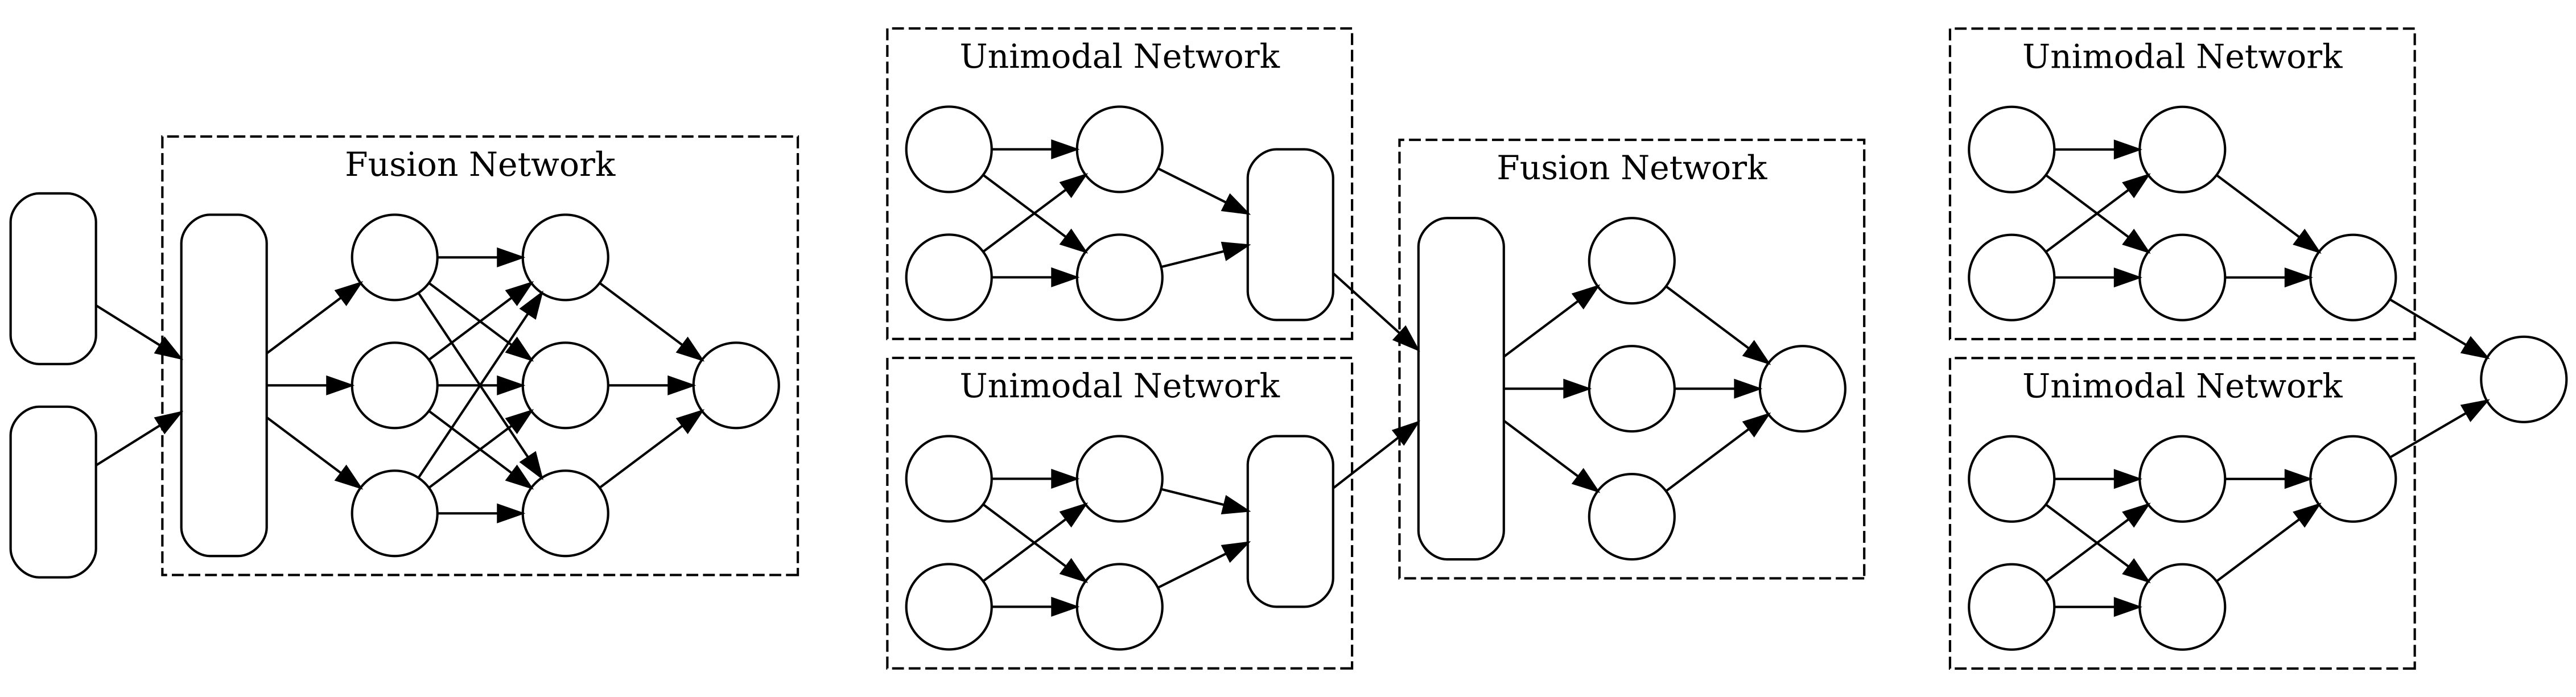
\includegraphics[width=\textwidth]{latex/fusion/all_fusion.png}
    \caption[Multimodal Fusion categories]{Illustration of different variants of fusion networks. Shown on the left is early fusion, intermediate fusion is shown in the middle and late fusion is shown to the right. The illustration was created with graphviz. \cite{Gansner2000Open}}
    \label{fig:fusion_graphs}
\end{figure}


\subsection{Biomarker Detection and Model interpretability}

Model interpretability is an important factor when developing modern deep learning systems, for which there are multiple reasons. By making a model interpretable, it is easier to trust its predictions but also helps to make it more accountable in case of false prediction. These tools help us to understand the prediction, and thus they make it possible to perform targeted changes aiming at improving the model. Another key aspect of interpretability is fairness. By understanding what features of the input the model is attending to, we can detect biases or, in some cases, discrimination with the potential of eliminating these deficits.
As we are interested in biomarker detection, feature attribution methods are most interesting to us. These methods can produce attribution scores for each feature of the input towards the output of the model. Hence, in a WSI, tissue regions of interest could be identified using such tools. For gene expression data, the equivalent would be genes that are especially important for prediction.

\subsubsection{Saliency}

By taking the derivative \(w\) of the image score with respect to the image itself per point in the image, we can obtain a set of weights that attribute the pixels that impact the prediction the most. The Saliency map \(M\) is computed by taking the maximum value of the derivative \(w\)  for each pixel across different channels of the input. This can be denoted as:
\[ M_{ij} = max_c | w_{h(i,j,c)}\]
where \(i\) and \(j\) denote the height and width dimension, and \(c\) the channels of the image. This approach does only require the trained model, a suitable input as well as the obtained score, thus no extra annotations are needed. Furthermore, computation of saliency is cheap as only a single back-propagation pass is performed. \cite{Simonyan2013Deep}
Such a map has the same dimensions as the corresponding input image and can therefore easily be overlaid on top of it.
An extension of saliency maps can be obtained by multiplying the gradient \(w\) by the values of the input, which is inspired by linear models. \cite{Shrikumar2016Not}

\subsubsection{Integrated Gradient}

Integrated Gradients (IG) defines two important axioms that attribution methods should follow to provide good results. The authors note that previous methods such as Saliency \cite{Simonyan2013Deep}, DeepLift \cite{Shrikumar2016Not} or Layer-wise relevance propagation (LRP) \cite{Bach2015Pixel} do not adhere to these axioms.

\paragraph{Defintion: Attribution}

IG defines attribution such that, for a pair of input \(x\) and baseline \(x'\), the attribution \(a_i\) of a single point \(x_i\) is the contribution of that point towards the prediction \(F(x)\). The baseline is needed as a reference point that always produces a neutral prediction. For image tasks, that could be a black image, but is task specific in the end.

\paragraph{Axiom a: Sensitivity}

This axiom demands that, if input and baseline only differ in a single value but still produce different predictions, the corresponding variable should be given a non-zero attribution. Furthermore, the opposite should also be the case. That is, when the alteration of a variable does not change the outcome of a function, it should always have zero attribution.  
Previous methods often fail to ensure this axiom is honored. Because they often rely on Backpropagation, non-linear activation functions, such as ReLU, will impact the process in such a way that this characteristic cannot be fulfilled. \cite{Sundararajan2017Axiomatic}

\paragraph{Axiom b: Implementation Invariance}

This characteristic describes that the attributions for an input should always be the same if the predictions are the same as well. Note that this should be the case for all inputs, i.e. the two networks are considered to be functionally equivalent. This means that this is the case irrespective of the implementation of the network itself, as it is situated between input and prediction (implementation-independence). The authors further use the chain rule as a comparison. \cite{Sundararajan2017Axiomatic} As, this rule states that a derivative can be computed directly or through some intermediaries, knowing the derivative of the intermediary is not essential to the final result. The neural network is compared to such an intermediary by the authors.

\paragraph{Methodology}

Formally, IG is given by the following, with \(\frac{\partial F(x)}{\partial x_i}\) representing the gradient of the neural network \(F(x)\) along the \(i^{th}\) dimension

\[
\text{IG}_i(x) = (x_i - x'_i) \times \int_{\alpha=0}^1 \frac{\partial F(x' + \alpha \times (x - x'))}{\partial x_i} d\alpha
\]

Practically, this can be described as accumulating the gradients between input \(x\) and its baseline \(x'\) along a straight path. Since this is computationally not possible, IG is approximated by summation of a set number of gradients along that path as follows:

\[
\text{IG}_i(x) \approx (x_i - x'_i) \times  \sum_{k=1}^M \frac{\partial F(x' + \frac{k}{M} \times (x - x'))}{\partial x_i} \times \frac{1}{M}
\]

This method can be easily computed, and the number of steps \(M\) defines the granularity of the approximation. As IG only depends on the gradients and not on the network, both axiom a and axiom b hold. \cite{Sundararajan2017Axiomatic}

\subsubsection{GradCAM}

Unlike Saliency Maps and IG, GradCAM is specific to convolutional networks. It assigns attribution values to each neuron for a particular network output with respect to any given convolutional layer of the corresponding CNN. However, usually the last convolutional layer in the network is chosen. 

For this purpose, the feature map activations $f_k(x, y)$ for input \(x\) and score \(y\) with respect to a convolutional layer \(k\) are obtained \textit{via} a single forward pass through the model. The importance weights \(\alpha_k\) of the neurons are then obtained by computation of the gradients \textit{via} backpropagation and combining them with global average pooling as follows

\[
\alpha_k = \overbrace{\frac{1}{Z}\sum_{i=1}^H\sum_{j=1}^W}^{\text{global average pooling}} \underbrace{\frac{\partial y}{\partial f_k(i, j)}}_{\text{gradients}}
\]

where \(Z\) is a normalization constant that ensures \(\sum_k \alpha_k = 1\) and \(H\) and \(W\) are height and width of the input, respectively. The authors describe \(\alpha_k\) as a partial linearisation of the neural network that captures the importance of feature map \(k\). These weights can then be used to obtain a coarse heatmap representing the importance of the inputs to the convolutional layer:

\[
\text{GradCAM}(x) = \text{ReLU}\left(\sum_k \alpha_k f_k(x)\right)
\]

By applying ReLU to the linear combination of weight and feature activation map, we filter for features with a positive influence. Hence, the intensity of these pixels has to be increased to increase the score \(y\). Negative values are likely to result in low attribution. \cite{Selvaraju2016Grad}

Guided GradCAM is a method described in the same publication. It adds the ability to produce fine-grained pixel-space visualisations.
As the matrix obtained from GradCAM has the same dimensions as the input of the considered convolutional layer, it is first upsampled to the dimensions of the input image to allow easy interpretation. The result is multiplied element-wise with the output of guided Backpropagation, another interpretability technique \cite{Springenberg2014Striving}. This fusion of methods produces a high resolution attribution map that determines fine-grained features but also stays discriminative, i.e. it still only attributes to the target task. \cite{Selvaraju2016Grad}

\subsubsection{Occlusion based attribution}

This is a straightforward perturbation based approach that differs fundamentally from the ones presented above. Perturbation methods usually compare the output of the model on the original and on an altered version of the image, to determine the role of the perturbed features. Occlusion based attribution involves replacing a contiguous rectangular region with a given baseline (e.g. an all-zero tensor), and computing the difference in output. \cite{Zeiler2013Visualizing} 

In implementation, this has the effect that the first patched perturbation is applied in the top left corner and then progressed using a sliding window that can produce overlapping regions.Thus, the final patch applied in a direction can be cut-off and thus will be smaller than the  other occlusion patches. The granularity of the attribution map can be defined by the kernel size and the stride. \cite{Zeiler2013Visualizing}

\subsubsection{Attention Mechanisms}

This method is unlike the previous ones, as it is a modification of the network architecture itself and thus learned with each iteration during training.
As we will see later, we use attention mechanisms as a method for feature selection during fusion. However, these methods can also be used for visualising the importance of different inputs. When using a patch-based network, we can apply a simple attention mechanism to determine the relevance of each patch. Thus, we can easily create an attribution map of WSI patches to find regions of high interest. With this technique, the patch size becomes a parameter for the granularity of the biomarker search. \cite{Ilse2018Attention} The advantage of this method is that the attribution of features is computed directly as part of the training process, no extra processing time is needed. However, it also has to be planned for when constructing the network and cannot be just applied as an afterthought, instead full retraining is required if added later to the network. 


\subsection{Neural Network architectures}

This section aims to give a brief overview over the types of neural network used in this work. 

\subsubsection{Residual Networks}

Residual networks are very popular networks for any kind of images analysis task. Originally introduced for classification tasks, they were introduced in 2015 by He \textit{et al.} \cite{He2015Deep} What these networks add to regular CNNs is the concept of a residual block. These blocks usually consist of multiple convolutional layers and their accompanying regularisation techniques (dropout, batch normalisation, etc.). Bypassing such a block is the input that is being processed. It is then added to the output of the block like so \[x_{l+1} = x_l + F(x_l)\] where \(x_l\) is the input to the block and \(F(x)\) is the applied mapping represented by the residual block. This introduces a bias towards the identity matrix of the input, which stabilises gradient propagation that is less impacted by \(F\). \cite{He2015Deep} 
When imagining the network as a space of functions which the network can represent, this allows to narrow down that space by adding complexity but ensures that the new space stays within the previous one at the same time. This way, we can ensure that more complex models will be at least as effective as their predecessor. \cite{Zhang2021Dive}
Another way of looking at it is, that the loss surface becomes much smoother by adding the so-called skip connections than without. \cite{Li2017Visualizing}

\subsubsection{EfficientNet}

The EfficientNet architecture is the result of a Network architecture search (NAS). 
During the search for EfficientNet, network width, network depth, and image resolution were systematically scaled up in a balanced manner. Importantly, the number of floating point operations per second (FLOPS) was directly included into the objective function of the NAS. \cite{Tan2019EfficientNet} This way, the resulting network architecture is supposed to prefer fast training times, hence the name of the network. A previous NAS result, MobileNet, inspired EfficientNet. However, MobileNet was optimized for time of inference or latency. \cite{Howard2017MobileNets, Sandler2018MobileNetV2}
The EfficientNet research shows that bigger input images need more layers to increase the receptive field and need more channels to capture more fine-grained patterns on bigger images. The resulting architecture managed to outperform ResNet on multiple tasks

With the updated version, EfficientNetV2, these results are further improved. By changing the architecture of the residual blocks, they improve the performance of the NAS and of the resulting network further. Originally, the same blocks as in MobileNet were used, and only their parameters were modified. Now, the NAS also looks for a combination between these kinds of blocks.
The authors conclude, that equally scaling up every stage of the network is suboptimal. When scaling up a model, the unequal contributions of layers need to be considered. 
They also argue that increasing the size of the data set is more important than increasing the size of the model in any way. \cite{Tan2021EfficientNetV2} 

\subsubsection{Self Normalising Networks}

These networks improve over regular feed forward or fully connected networks (FNN, FCN). The authors claim that such 
FNNs only perform well if they have a low number of hidden layers. \cite{Klambauer2017Self} This limits the possible level of abstraction and complexity that the networks can represent.
Self-Normalising Networks (SNN) aim to improve upon this by ensuring the following property: each activation maps mean and variance from one layer to the next. Furthermore, outputs stay in the domain of the input, and all points in this domain converge towards a single fixed point. 

\noindent The authors achieve this by combining a scaled exponential linear unit (SeLU) with a new type of layer, which they propose as alpha dropout. The formula for SeLU is given by

\[
\mathrm{SeLU}(x) = \begin{cases}
  \lambda x & \text{if } x > 0, \\
  \lambda \alpha (\exp(x) - 1) & \text{if } x \leq 0,
\end{cases}
\]

\noindent where \(\lambda\) and \(\alpha\) both are scaling factors that help ensure the following conditions required for SNNs

\begin{compactitem}
    \item The presence of negative and positive values are needed to control the mean.
    \item SeLU imposes a lower bound on outputs to dampen the variance.
    \item A slope larger than one to increase the variance if it is too small.
    \item A continuous curve to ensure a fixed point of convergence to exist.
\end{compactitem}

\noindent Alpha dropout is a modification of regular dropout to enable the maintenance of the original mean and variance of the input. Nodes that are selected by the dropout mechanism, get randomized on every forward call, and scaled and shifted to maintain zero mean and unit variance. the authors prove that, with this new regularization scheme, their network outperforms other FNNs with other normalization techniques at a higher number of hidden layers. \cite{Klambauer2017Self}


\subsection{Training Techniques}


\subsubsection{Adam Optimiser}
The Adam optimiser is a gradient-based optimisation algorithm that aims to improve stochastic gradient descent (SGD). The algorithm uses an adaptive learning rate method that is different from traditional SGD algorithms. It maintains exponential moving averages of the gradient and the squared gradient. These are estimations of the first moment (mean) and the second 'raw' moment (non-centred) variance, respectively.

The update rule for the Adam optimiser can be expressed as follows

$$ \theta_t = \theta_{t-1} - \frac{\alpha}{\sqrt{\hat{v}_t}+\epsilon}\hat{m}_t $$

where $\theta_t$ is the parameter vector at time $t$, $\hat{m}_t$ and $\hat{v}_t$ are the bias-corrected first and second moment estimates of the gradient at time $t$, $\alpha$ is the learning rate, $\epsilon$ is a small positive constant used for numerical stability, and $t$ is the iteration number or time. The bias-corrected estimates $\hat{m}_t$ and $\hat{v}_t$ are computed as

\[ \hat{m}_t=\frac{m_t}{1-\beta_1^t},\ \ \ \ \ \ \hat{v}_t=\frac{v_t}{1-\beta_2^t} \]

where $m_t$ and $v_t$ are the first and second moment estimates of the gradient at time $t$, and the hyperparameters $\beta_1$ and $\beta_2$ control the exponential decay rates for the first and second moment estimates, respectively. This bias-correction is necessary due to the initialisation of $\beta_1$ and $\beta_2$ with zero. The raw first and raw second moment estimates are calculated as follows

\[m_t = \beta_1 m_{t-1} + (1 - \beta_1) g_{t}, \ \ \ \ v_t = \beta_2 v_{t-1} + (1 - \beta_2) g_t^2\]

Here, $g_t$ represents the gradient with respect to the objective function at time $t$, and $\beta_1$ and $\beta_2$ are hyperparameters that control the exponential decay rates for the estimates of the first and second moments, respectively. $m_t$ and $v_t$ are both initialised with zero. \cite{Kingma2014Adam} This algorithm is a combination of Root Mean Square Propagation (RMSP) \cite{Hinton2012RMSProp} and AdaGrad. \cite{Duchi2011Adaptive}

AdamW is a modification that adds weight decay to the algorithm. The authors stress that there is a conceptual difference between weight decay and the commonly used $L_2$ regularisation. The authors further argue that weight decay behaves the same as $L_2$ regularisation only if weight decay is coupled to the learning rate, as done in the PyTorch implementation of Adam. Due to dynamic learning rate updates within the Adam algorithm, this can lead to worse generalisation performance than SGD with momentum. as SGD does not suffer from this problem.
AdamW proposes to decouple the weight decay from the gradient-based update. This leads to better generalisation. The authors further note, that AdamW still benefits from a global learning rate schedule. \cite{Loshchilov2017Decoupled}

\subsubsection{Mixed Precision Training}
Mixed precision training is a technique that makes use of smaller data types during the training of a model, which brings two advantages. First, the overall memory requirements are lowered significantly. This enables increased batch sizes, larger models, or larger inputs. More specifically, the inputs and weights are converted to a half-precision data type (float16) before performing the forward pass of the model. The intermediate activations, which are the results of the matrix multiplications and nonlinear activation functions, are also converted to float16 before being passed to the next layer. During the back-propagation of gradients, the gradients are accumulated in single-precision format (float32) to avoid numerical underflow. The accumulated gradients are then converted back to float16 before being used to update the weights of the model. This way, the memory consumption can almost be halved. \cite{Micikevicius2017Mixed}
Second, the training time itself can be reduced. Due to the reduced amount of decimals that need to be approximated, calculations can be done faster. Furthermore, energy requirements are also significantly reduced. \cite{Micikevicius2017Mixed}, \cite{Tagliavini2017Transprecision}
The special \verb|bfloat16| data type was first proposed in 2017 for mixed precision training. This data type preserves the same amount of exponent bits as the IEEE 754 single-precision 32-bit float by solely truncating the mantissa. This stands in contrast to IEEE half-precision 16-bit float, where both exponent and mantissa are truncated, but the mantissa by less fields. This allows the bfloat16 data types to represent the same value range as a regular 32-bit float. \cite{Tagliavini2017Transprecision}
Kalamkar \textit{et al.} were able to show, in 2019, that using this data type achieves the same results as non-mixed precision training. When using the regular 16-bit float, hyperparameter tuning would usually be necessary to achieve this. \cite{Kalamkar2019Study}


\subsubsection{Stochastic Weight Averaging}
Stochastic weight averaging (SWA) is a technique that helps to improve the generalisation of Stochastic Gradient Descent (SGD) and related algorithms.

SWA performs an equal average of the weights traversed by SGD with a modified learning rate schedule. This helps avoid convergence towards the boundary of a minimum. This is especially helpful when the loss surface around the minima resembles a plateau. There, SGD might fail to find a meaningful direction on the gradient. In essence, the weights corresponding to the minimum learning rate per cycle are averaged. \cite{Izmailov2018Averaging}

A variant of SWA is called fast-SWA. After a certain number of training steps within a cycle, the learning rate is adjusted to a lower value. Then, the running average of the weights visited by the optimiser is maintained for the remainder of the cycle and used for further steps. Using this average can be interpreted as simultaneously considering multiple solutions provided by the optimiser; which are the steps since the activation of fast-SWA. since those Solutions lie closer to the boundaries, SWA will help find the centre and thus a better minimum. This has been shown to improve generalisation in computer vision tasks. \cite{Athiwaratkun2018There}

\cleardoublepage

%% related Work
\chapter{Related Work}\label{related}

This section aims to give an overview over various neural network techniques that analyse whole slide images and perform survival analysis, while going into further detail for a few cases, where multimodal fusion models have been employed. Finally, some preliminary findings related to clear cell renal cell carcinoma are summarised. 

\section{Survival Analysis and Neural Networks}
The first adaption of survival analysis, based on the Cox proportional hazards model, dates back to 1995. Farragi and Simon used a network with a single hidden layer and varying numbers of hidden nodes to maximise a partial likelihood function derived from the CPH formulation. The C-Index was chosen as the performance metric. With only 3 covariates as input (age, weight, and stage of the disease), they were the first to overcome the linearity constraint of the CPH model, but were unable to significantly outperform the traditional model, achieving a c-index of 0.661. \cite{Faraggi1995neural}

The authors of DeepSurv claim to be the first to apply modern deep learning techniques to the Cox proportional hazards loss function. Unlike Farragi and Simon, they manage to outperform the linear CPH model as well as Random survival forests (RSF), a machine learning method, that had been adapted to survival analysis in the meantime. DeepSurv is a multilayer network that alternates between fully connected and dropout layers, with a linear layer that predicts the output of the log-risk function. Furthermore, they develop a treatment recommender system that uses DeepSurv's results. \cite{Katzman2018DeepSurv}

The DeepHit model is a multitask network in the sense that it can handle multiple potential causes of the event smoothly. This is done my partitioning the network in a shared and $K$ cause-specific subnetworks. 
The fully connected head of the network then performs a prediction based on the output of each subnetwork as well as on the original covariates. Additionally, they use the time-dependent concordance index ($C^{td}$ Index) for measuring the performance. In comparison with the ordinary concordance index, the $C^{td}$ index is capable of reevaluating the risk of an individual over time; the c-index is computed only at the initial time of observation. Ultimately, this achieves to lift the proportionality constraint of the classical CPH model. \cite{Lee2018DeepHit}

\section{Deep learning on WSIs}

Due to the high size of these images, it is unlikely that they will fit into GPU memory at full resolution. Hence, there are two general approaches to dealing with these images. 
Either they are downsampled to a lower resolution or they are divided into patches. In the latter case, the patches can then be processed separately or only a subset of them is used at all.

\subsection{Convolutional Neural Networks (CNN)}

The most straightforward approach is to use convolutional neural networks (CNN). In general, they are commonly made up of multiple blocks of convolutional, pooling and non-linear activation layers. This section's purpose is to extract features from the input. At the “head” of such a network, usually there are few fully connected layers. These sections aim to perform the actual task of the network, some form of prediction. However, these approaches are usually only effective when tissue-annotations are available at the time of training. One issue with the use of CNNs is that it is rather difficult to interpret the meaning of the extracted regions. \cite{Lipkova2022Artificial}
In contrast to CNNs, the following methods tend to not require strong supervision to work well and slide level annotations are sufficient. 

\subsection{Graph Convolutional Networks (GCN)}

A graph convolutional network can be constructed from parts of the images. These can be detected cells, tissue regions, or patches of the WSI. The distance of these objects is then used to define the length of the respective edges. \cite{Chen2022Pathomic, AhmedtAristizabal2022survey, Chen2021Whole}
This approach enables us to incorporate global context in the input to the network. In contrast to a regular CNN, these networks operate on unstructured graphs. 
\cite{Lipkova2022Artificial} Images can be considered graphs with 4 or 9 edges, depending on the definition.
Compared to downsampling the WSI for a CNN, we can choose the structure to be considered in the construction of the graph. Although the approach of construction is also a caveat of these networks, as it adds a collection of new hyperparameters that need to be tuned. 

 \subsection{Multiple Instance learning (MIL)}

In multiple instance learning, multiple inputs are grouped as 'bags'. The label to be predicted is assigned to the bag as a whole. It is to be noted that usually not all members of a bag have to conform to their bag's label. Such bags are sometimes referred to as 'negative' and the bags that only contain samples correctly associated are called 'positive'. A useful addition to this approach is to use an attention mechanism to determine the importance of patches toward their respective bag labels. \cite{Ilse2018Attention}
One such approach is introduced by Li \textit{et al.} in 2021. Here, the authors utilise the principle to detect tumours in image patches extracted from WSIs. They do this in a two-step process. The extracted patches are fed into a CNN to perform self-supervised contrastive learning. The pre-trained model is then re-used to obtain instance embedding of these patches. Interestingly, this is done twice, with the only difference being the scale of magnification of the WSIs. Embeddings obtained at 5x and 20x resolution are generated, each 20x patch has a corresponding lower resolution 5x patch. Then, each 20x embedding is concatenated to the corresponding 5x embedding and processed by the MIL aggregator. This aggregator consists of a masked non-local block and a max-pooling block. While the latter determines critical instances based on their individual scores, the former measures the distance of each bag-member to the critical instance and produces a bag embedding. Both aggregated and critical instances are individually scored, and their scores are then averaged. For classification, this approach seems to work very well. On the Camelyon16 dataset, an accuracy of 0.89 is reached. \cite{Lu2021Data}
This approach might not be suitable for survival analysis, since we would like to consider all the information in the image. For classification this might be sufficient because the slide class can be predicted based on a small subset of each WSI.

\subsection{Vision Transformers}

These models use attention-based learning. Context awareness allows accounting for correlations between image patches and thus learn positional encodings. After learning spatial structures of patches, usually there are self-attention layers to determine the importance of the individual patches. This can be followed by a Multi-head attention layer, which uses multiple self-attention blocks in parallel to account for different kinds of interactions between the patches.
This works by assigning multiple tokens to each patch, one for the positional information and another for the true outcome (e.g. class). Together with their respective tokens, these tokens are simultaneously used as input to the network. \cite{Lipkova2022Artificial} There are quite a few implementations of these kinds of networks already. \cite{Chen2022Scaling, Chen2021Multimodal, Dosovitskiy2020Image}

\subsection{Autoencoders}

Autoencoders are self-supervised models that do not need labels for training, they find a joint latent representation of the input. Thus, they present an alternative to direct modelling. \cite{Stahlschmidt2022Multimodal} The most simple variant consists of an Encoder and a Decoder. The Encoder is a CNN that learns a lower-dimensional representation of the input. The Decoder uses the inverse operations of the Encoder and learns to reproduce the original image using the latent code as input. Methods based on this simple principle can be used for various appliances: generating artificial training data \cite{Chen2022Fast}, recreating missing image patches based on their neighbouring patches \cite{Lipkova2022Artificial}, or generally improving the performance of downstream tasks that are heavily based on the performance of a CNN. 
Another way to use these methods is as a means of compression. Since the full WSIs are too big to be loaded at once, individual patches can be compressed and their embedding vectors are used for the downstream task instead. Tellez \textit{et al.} trained, among others, a Variational Autoencoder (VAE) and a Bidirectional Generative Adversarial Network to compress patches into 1-dimensional feature vectors. They then compressed these vectors into a 3D matrix, with each vector's position corresponding to that of the original image. With this new tensor, a CNN was trained to predict tumour metastasis and tumour proliferation speed. \cite{Tellez2019Neural}
Variational Autoencoders (VAE) provide significant improvement with little change. Instead of learning a direct representation of each input, by adding noise, the encoder learns to model the latent space as a Gaussian distribution. Hence, the network learns the mean and variance of the data. The Gaussian distribution characteristic is ensured by the Kullback–Leibler (KL) divergence, which is added to the regular reconstruction loss. The KL divergence measures the difference between latent space and a standard Gaussian distribution. \cite{Kingma2019Introduction}

\section{Multimodal deep learning}

As seen in the previous section, there are a variety of available techniques. Their composable nature leads to an even greater variety of pipelines that are employed in research, to the point that even exact replications of parts of a previous analysis are rare. Here, we look at some examples incorporating multimodal fusion.
\subsection{Siamese Network and Multimodal dropout} 
In 2019 Cheerla \textit{et al.} applied late fusion using four different datasets. These were gene expression data, miRNA data, clinical data and whole slide images. Moreover, they used three very different architectures, with only the subnetwork for gene expression and miRNA data sharing similarities. They calculate the colour balance of patches to remove the empty ones. Then, they select a subset of patches for each sample to be used for training. As not all modalities are available for each sample, they introduce what they call multimodal dropout. This technique trains the DNN to deal with missing modalities. By purposely removing whole modalities prior to fusion with probability $P=0.25$. This way, the network is forced to create representations that are robust to missing data. The fusion is guided by the sum of the pairwise similarity loss. Furthermore, by pre-training their fusion method using a loss inspired by the cosine similarity, they force same-patient feature representations from different modalities to resemble each other.
This work achieved a c-index of 0.73 for RCC cases from the TCGA-KIRC dataset, where the use of multimodal dropout did not affect this metric. TCGA-KIRC was the only one of the 20 Cancer data sets analysed where this was the case. Also, with only two exceptions, multimodal dropout improved the c-index by a one-digit percentage. It only decreased for TCGA-KICH and TCGA-THCA, but both already showed a very high c-index $\ge$ 0.90 which they managed to maintain despite their drop in performance.
Also, noticeable are the general variations in Performance on different TCGA cancer datasets. Although the TCGA-KICH dataset achieved a c-index of 0.93 (with multimodal dropout), for the TCGA-LUSC dataset only 66\% of predictions were concordant. The autors  found that molecular data alone already provides relatively high performance. \cite{Cheerla2019Deep}
\subsection{PathomicFusion} 
Another approach was proposed by Chen \textit{et al.} in 2020. They combined WSIs, genomic features and a graph constructed from the WSIs. The interesting parts are the use of Self-Normalizing Networks (SNN) for the processing of the genomic information, as well as the graph network. For the former, the network uses scaled exponential linear units (SeLU) over the more common ReLU as activation function. This has the effect that outputs are pushed towards zero mean and unit variance. In combination with alpha dropout, self-normalising property is maintained. The aim behind this setup is to lower the risk of overfitting, which would be quite high otherwise. 
The graph is constructed by detection and localisation of cells via nuclei segmentation. Then, using the K-nearest-neighbours algorithm, the edges were drawn to the five closest neighbours of each cell. The underlying assumption is that cell-cell interactions are most relevant between those that are adjacent. Each cell in the graph is then associated with up to 24 pre-defined features. This network is then used to learn a representation of the WSI. Obviously, this approach cannot contain the same information the WSI does, which is why both are used in the fusion. Fusion is handled by computing the Kronecker product to model pairwise feature interactions of all inputs. The resulting vector is then used for the Cox regression. In addition, the authors use GRAD-CAM \cite{Selvaraju2016Grad} and Integrated Gradients \cite{Sundararajan2017Axiomatic} to inspect the feature attribution of WSIs and genomic features respectively. \cite{Chen2022Pathomic}
\subsection{Multimodal Co-Attention Transformer (MCAT)} 
In 2021, Chen \textit{et al.} proposed another approach that utilizes early fusion between histology and genomic data. For this, both inputs are processed first by a CNN or fully connected layers respectively. This produces embeddings of genomic features and WSI patches. They are then processed in a co-attention mechanism guided by the genomic embeddings to learn pairwise interactions between the instance-level histology patches and genomic embeddings. Then a so-called set-based MIL transformer is used to obtain risk scores based on both embeddings. The co-attention mechanisms make visualisation of high- and low-risk cases possible, based on the attention score of each image patch. Heatmaps are overlaid onto the WSI, locating regions of high attention with granular detail. Although the approach seems very interesting, the c-indices for different datasets are mostly low. Although the Glioblastoma \& Lower Grade Glioma (GBMLGG) dataset scored a c-index of 0.82, none of the other four datasets surpassed 0.62. That being said, the authors compare their results to other MIL approaches and receive the best results with only one exception. \cite{Chen2021Multimodal}
Perhaps, MIL is not well suited for survival analysis in general, as these methods usually do not provide a “full picture” to the network and, unlike autoencoders, do not control the content of the latent space. 
\subsection{Long short-term memory (LTSM)} 
Ren \textit{et al.} use long short-term memory (LTSM) networks, a subtype of recurrent neural networks (RNN), to model the features of the multimodal input and for survival analysis on the recurrence-free survival (RFS) in months. For this, the authors incorporated ROI-extracted image patches and pathway activity data in a multimodal manner. Therefore, genomic data were first analysed with statistical methods to obtain so-called pathway scores. These were then fed together with the selected image patches into the neural network via simple concatenation of vectors, which then served as input into the LTSM. With this architecture, a c-index of 0.74 was reached. \cite{Ren2018Recurrence}
\subsection{MultiSurv} 
The MultiSurv model is another end-to-end multimodal network where the authors compare six different fusion methods. The feature vectors of each modality are fused using concatenation, row-wise summation, multiplication or taking the row-wise maximum. The last two approaches are more involved. First, an attention mechanism is used. This uses a fully connected linear layers followed by the hyperbolic tangent activation function and SoftMax rescaling. \cite{ValeSilva2021Long} Such a layer does not reduce the size of its input, but rather learns the importance of each node for the outcome of the downstream and balances them accordingly. The last approach is based on another publication. EmbraceNet uses so-called docking and embracement layers to fuse individual feature vectors. The docking layers take an output vector of an independent modality-specific network and resizes them to a common size. The embracement layers then pool individual values from each input to produce a vector of the same size as one of the input vectors. This is achieved by using the summed Hadamard product between a vector that has been preprocessed by the docking layers and a vector drawn from a multinomial distribution, this ensures that all values add up to one. The sum of such a Hadamard product then forms a single value in the final feature vector. \cite{Choi2019EmbraceNet}
Also, they use a discrete-time survival model to be able to adjust the predictions after one or more of these discrete time intervals have passed. This is done in order to remove the proportionality constraint 
On unimodal data, Multisurv manages to outperform the linear CPH model, RSFs, Deepsurv and DeepHit for a majority of modalities. Interestingly, the best results were achieved when not all six available modalities were used. In the author's direct comparison of MultiSurv and DeepSurv they achieved a $C^{td}$ index of 0.801, which is higher than the c-index of DeepSurv on the same dataset. \cite{ValeSilva2021Long}

\clearpage

\section{Clear cell renal cell carcinoma (ccRCC)}

Chen \textit{et al.} came to an interesting conclusion with respect to ccRCC. They found that a decrease in CYP3A7 expression as well as an increase in the expression of PITX2, DDX43 and XIST are correlated with the risk of developing cancer. Furthermore, they conclude that vasculature and cell atypia are important features for survival outcome prediction. They were able to show that cells with indiscernible nucleoli are more common in patients with longer survival, while large cells with clear nucleoli are indicative of patients with shorter survival. \cite{Chen2022Pathomic}

In 2015, Christinat \textit{et al.} used microRNA (miRNA) for classification and were able to identify subgroups of ccRCC. They found six distinct patient clusters, each with different clinical outcomes, pathological features and somatic mutation profiles associated to them. These groups were identified by applying the log-rank test to the miRNA expression levels. \cite{Christinat2015Integrated} This work illustrates the importance of tumour heterogeneity. Although we classify two patients as having the same disease, the cellular characteristics can be completely different. This nonlinearity threatens that miss-treatments occur and the overlook of individual factors. Thus, we should ask whether a more fine-grained classification of cancer types is needed to properly address the full spectrum.




\cleardoublepage

%% 
%%%%%%%%%%%%%%%%%%%%%%%%%%%%%%%%%%%%%%%%%%%%%%%%%%%%%%%%%%%%%%%%%%%%
% Grundlagen
%%%%%%%%%%%%%%%%%%%%%%%%%%%%%%%%%%%%%%%%%%%%%%%%%%%%%%%%%%%%%%%%%%%%

\chapter{Material and Methods}
  \label{MetMat}

\section{Data}
  \label{Data} 
  
\subsection{Data acquisition}
  \label{DataAcq}

The original Dataset consists of 947 whole slide images from 176 Patients. The patients were treated at the Hannover Medical School (MHH) hospital between 1992 and 2022. Most images have region-level annotations associated to them that define the tissue and the tumour areas at different levels of granularity.
For a subcohort of 24 patients, expression counts of cancer-relevant genes are also available. These were acquired using the NanoString panel nCounter\textsuperscript{\textregistered} PanCancer IO 360\texttrademark. This assay comprises 770 genes that are categorised into 16 categories, each belonging to either one of the groups 'Tumor', 'Microenvironment' or 'Immune Response'. A subset of 20 genes makes up an internal reference. \cite{NanoStringTechnologies2017Gene}
Figure \ref{fig:SurvStats} visualises both the subcohort with their respective survival times and the overall distribution of patients  with respect to their survival times.

\begin{figure}[htb]
    \centering
 \begin{subfigure}[b]{0.59\textwidth}
 \centering
    \includegraphics[width=\textwidth]{latex/figures/survival_days_distribution_hires_evenly_binned.png}
     \caption{Distribution of survival times}
     \label{fig:SurvHisto}
 \end{subfigure}
    \hfill
 \begin{subfigure}[b]{0.4\textwidth}
 \centering
     \includegraphics[width=\textwidth]{latex/figures/surv_race_rcc.png}
     \caption{Survival time of subcohort}
     \label{fig:SurvRaceSmall}
 \end{subfigure}
  \caption[Cohort visualisation]{Distribution of survival times and concrete survival times of patients with gene expression data. An extension of \ref{fig:SurvRaceSmall} for the full cohort can be found in the appendix \ref{fig:SurvRaceFull}}
  \label{fig:SurvStats}
\end{figure}


\subsection{Pyramidal Images as SVS files}

The image files are provided as ScanScope Virtual Slides (SVS) files. This is the file format used by Aperio scanners for glass microscope slides. They represent a modification of regular TIFF files, such as altered tag structure and additional metadata. These files also use JPEG2000 or JPEG. This makes it feasible to store them in files smaller than 4 gigabytes. This is necessary as the underlying TIFF file format only supports file sizes below that threshold. \cite{AperioTechnologies2008Digital} TIFF files can hold multiple images with different sizes. Therefore, it is possible to bundle the same image at different resolutions within the same file. \cite{Aldus1992TIFF} 
This can practice can commonly be found in pathology image to represent different downsampling scales of the same slide image. Figure \ref{fig:pyramid}
However, due to the complexity of the file format, there are multiple possible ways to internally represent an image hierarchy in such files. \cite{Aldus1992TIFF} 
For example, the lower resolution files can be stored as extra 'pages' or as 'subfiles'.
This, in turn, limits the interoperability of different TIFF-based file formats used for digital pathology. It also increases the development burden on the applications and tools dealing with these files. The same problems occur for the metadata provided with each file, for example, SVS files use the TIFF metadata-tag “ImageDescription” to store information as key-value pairs. \cite{AperioTechnologies2008Digital} Meanwhile, the competing “OME-TIFF” format manages to store the meta-information formatted as XML within that tag. \cite{OpenMicroscopyEnvironment2022OME} 

\begin{figure}[h!t]
    \centering
    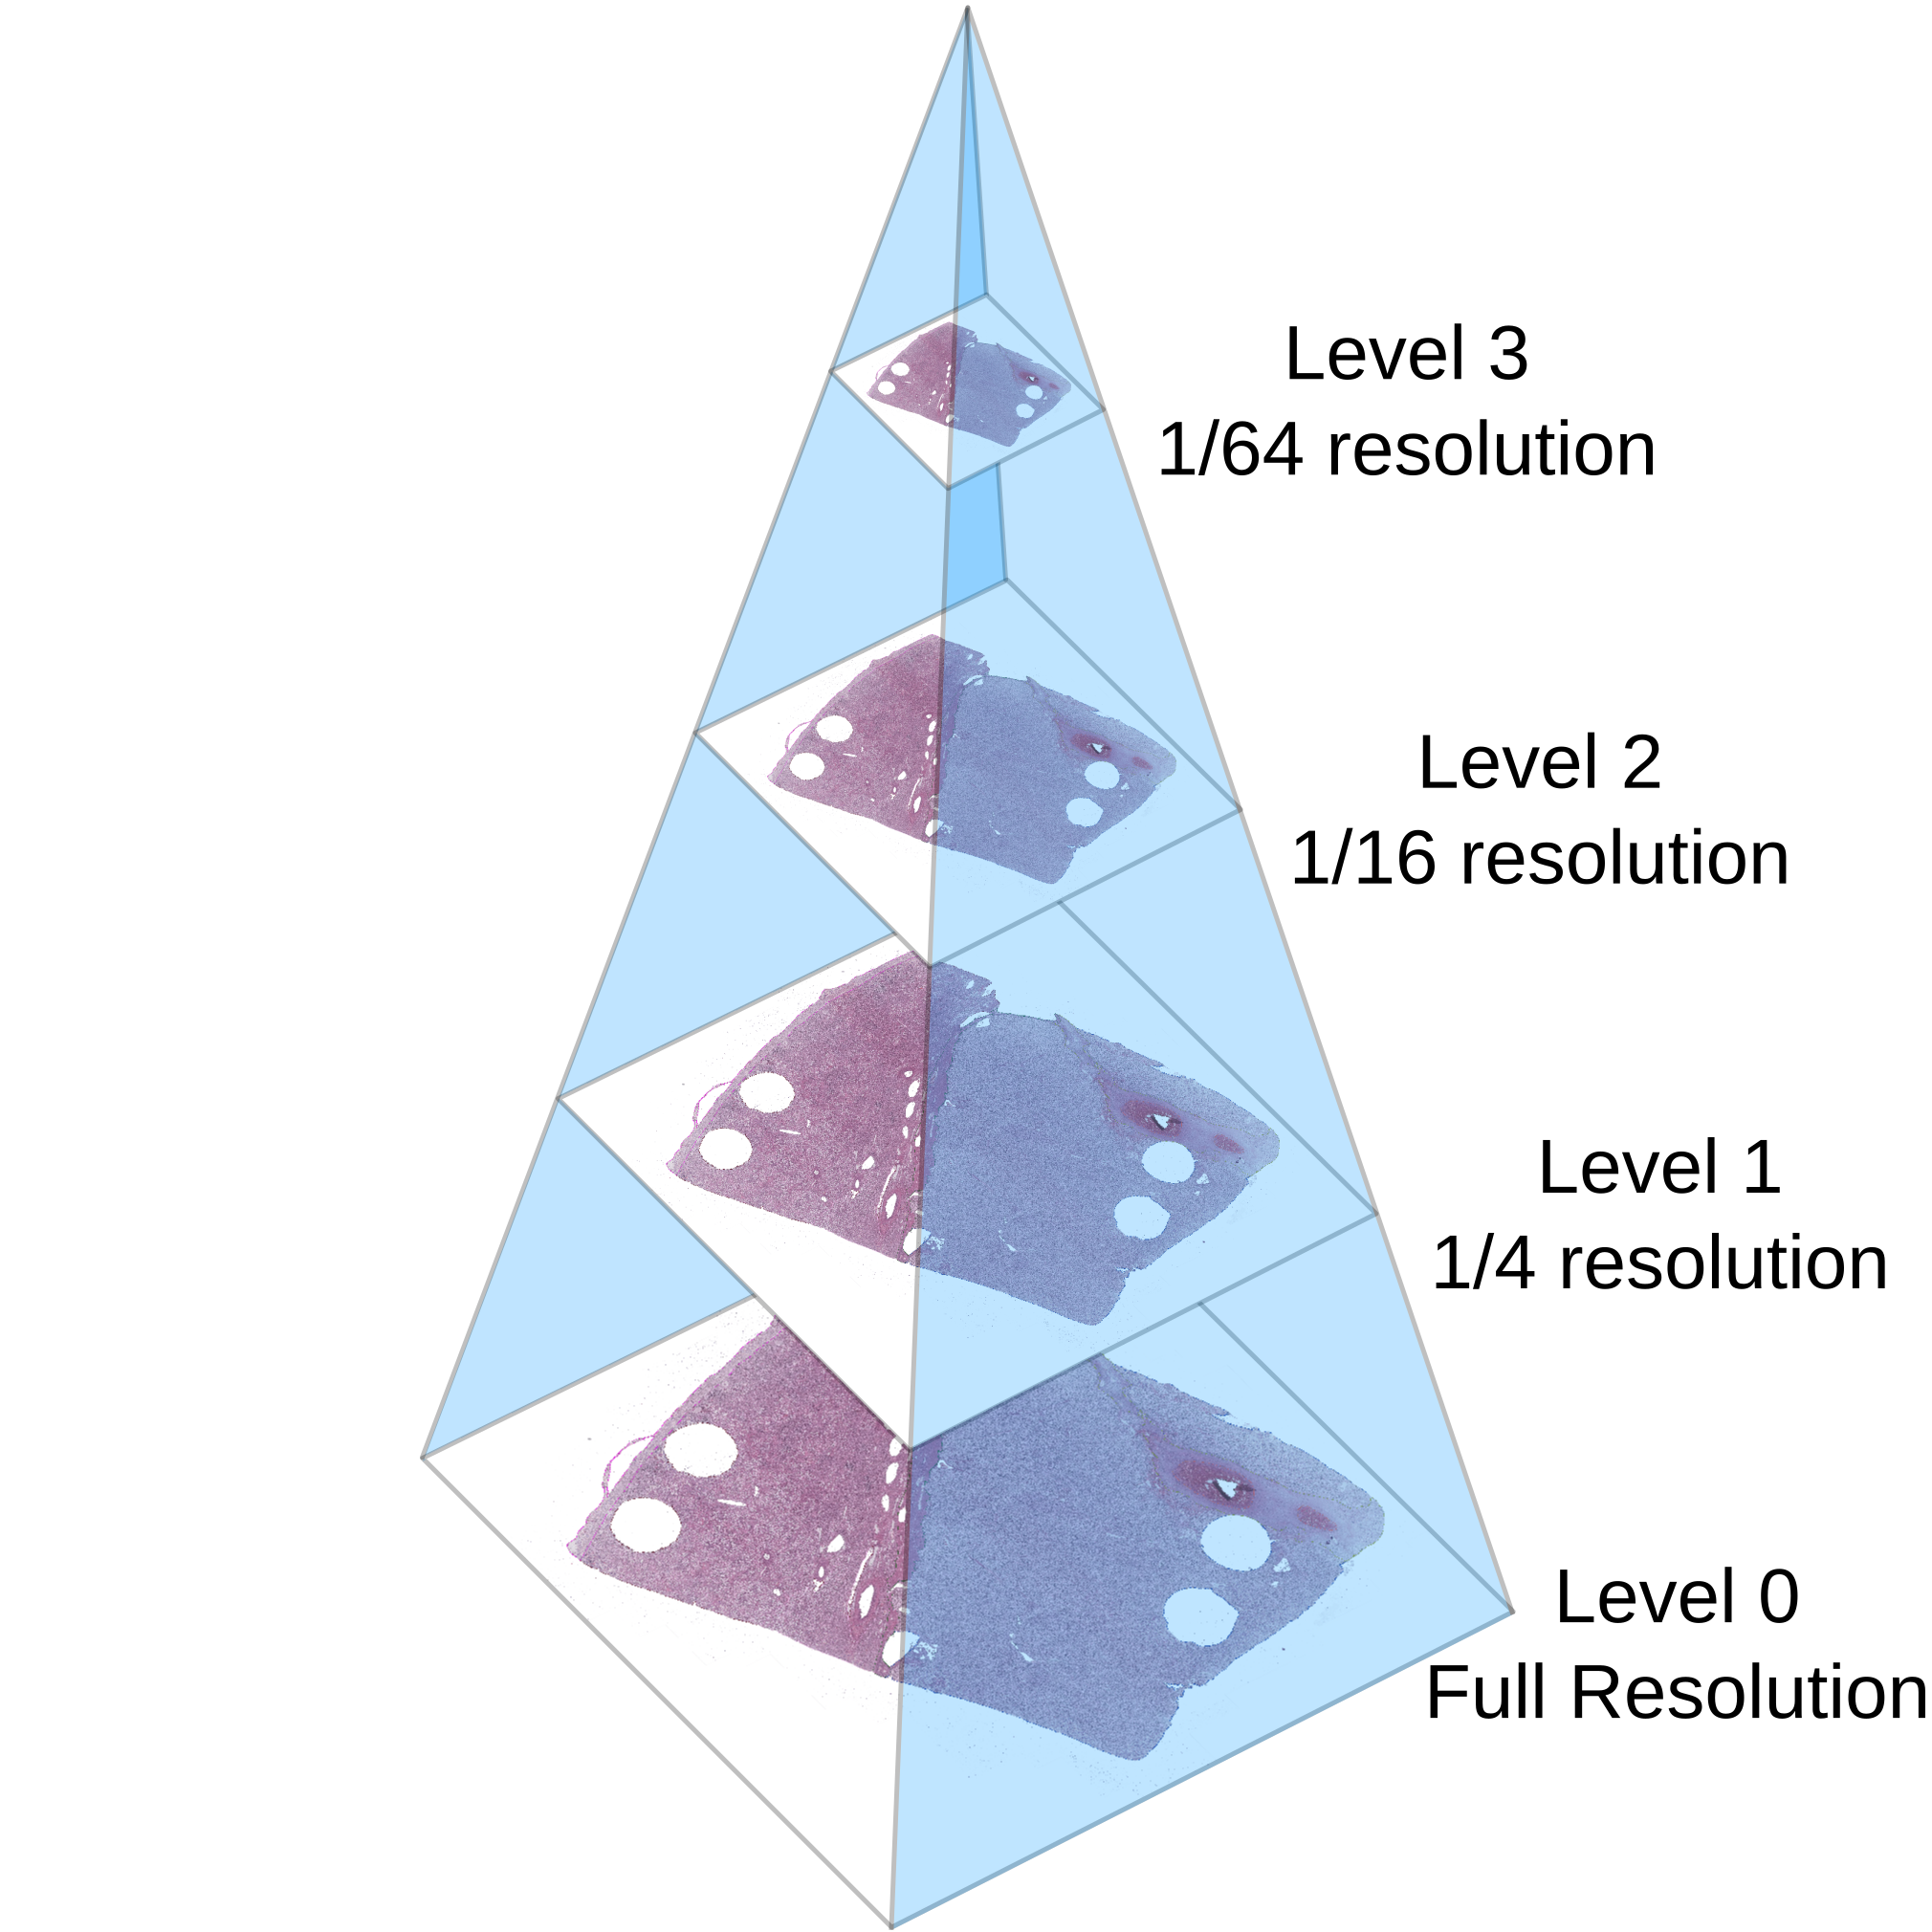
\includegraphics[width=0.6\textwidth]{latex/figures/Image_pyramid_centered.png}
    \caption[Pyramid representation of TIFF files]{Pyramid illustration of SVS files. The SVS format downsamples images by a factor to the power of four and saves them as separate pages. The page at index 0 contains the full resolution image, index 1 contains a special thumbnail. The following indices are used for the downsampled versions. Adapted from 'Illustration of an image pyramid with 5 levels.' by Cmglee (CC BY-SA 3.0). \cite{CreativeCommons2007Attribution, Cmglee2015Illustration} The figure was modified using Inkscape (version 1.2.2), a free and open source vector graphics editor. \cite{InkscapeTeam2022Inkscape}}
    \label{fig:pyramid}
\end{figure}

\subsection{Annotations and the GeoJSON file format}

The WSIs were annotated using the software QuPath, which was created for dealing with pathology images. \cite{Bankhead2017QuPath} Because of that, the annotations are not easily accessible and first have to be extracted from the respective QuPath projects. 
The python library \verb|paquo| was used to extract these individual annotations and export them as GeoJSON files. As the name suggests, the GeoJSON file format was originally invented to deal with high-resolution satellite images. \cite{Butler2016GeoJSON} Coincidentally, digital pathology images have a similar need for a lightweight, easy-to-parse file format to carry spatial information. The name also suggests that this is derived from the JSON file format. In fact, these files are valid JSON documents with pre-defined structures and names for keys and values. These files consist of an array of region objects and are made up of one or multiple arrays of coordinates that define one region's outline. In addition, each array is associated with various metadata; the individual keys are defined by either QuPath or the GeoJSON specification. \cite{Butler2016GeoJSON, Bankhead2017QuPath}. Only a subset of available annotations is used for this thesis. Those are the ones deemed most relevant to the task of the DNN. Concretely, the annotations are “Angioinvasion”, “Tissue”, “Tumor necrosis”, “Tumor regression” and “Tumor vital”. Figure \ref{fig:downsample_overlaid} shows a few examples of WSI with those annotations overlaid in the specified order. The medical interpretation is self-explanatory for most annotations. As Angioinvasion is the spread of tumour into a blood vessel, these annotations are generally much smaller in area and also rarer to occur than the regular tumour annotations.

\begin{figure}[h!t]
    \centering
    \includegraphics[width=0.32\textwidth]{latex/tissue/postproc_subimage_90-19_noLabel.png}
    \includegraphics[width=0.32\textwidth]{latex/tissue/postproc_subimage_109-42.png}
    \includegraphics[width=0.32\textwidth]{latex/tissue/postproc_subimage_19-42_noLabel.png}
    \caption[WSI and overlaid masks]{Tissue slides with annotations overlaid. The tissue annotation is only visible in areas without other annotations. It can be assumed that any non-white area of the image is marked as tissue. All images are taken at the same scale.}
    \label{fig:downsample_overlaid}
\end{figure}

\subsection{Data quality}

Multiple samples had to be removed from the dataset for reasons stemming from various issues with the data.

\subsubsection{Patient filtering} 
Data from whole patients had to be removed for two reasons. For once, this included patients who were affected by a cancer subtype other than the most prevalent one. Thus, only patients who were affected by clear cell renal Cell Carcinoma (RCC) were considered in this work. That is, because the morphological differences with other subtypes are too large and their subcohorts are too small in sample size to foster significant learning. This aspect reduced the number of patients from 176 to 141. 
In addition, not all the images provided were part of the study. Some images did not belong to the cohort of RCC patients at all, and others lacked any occurrence in one of the provided QuPath projects. Images of Patients that do not occur in any QuPath project also do not have any annotations. 
The second reason for removing patients is more pragmatic. In those cases, the necessary data for performing survival analysis is missing. For example, the time of the nephrectomy, which was used as the starting time, was missing.

\subsubsection{Image filtering} 
Next is the quality of the annotations. Since they are used for tissue segmentation, it is critical that they are present and usable. There are three reasons why patients were excluded from the analysis based on tissue-level annotations. First, 4 of the extracted GeoJSON files were empty. Most probably, because the image did not get properly annotated in the first place. Next, there were cases where only the tissue annotation is missing. This occurrence manifested in two forms. In the first case, the whole tissue-related entry in the GeoJSON file is missing, which happened in another 4 cases. However, some files do carry odd annotations that were only missing a classification. Whether that (or which, in the case of multiples per file) is the tissue-level one is difficult to determine without manual inspection by a domain expert. Therefore, these 13 images were also excluded.
The complete data provided consisted of 947 images and 176 patients. In the end, 705 images remained, out of which 495 belonged to the uncensored patients. The MHH provided up to five WSIs of different stains, consisting of one H\&E stain and four images stained with immunohistochemistry (IHC) staining. However, as explained above, not all patients had five usable images. 
This affected the balance of the resulting data sets at the slide level, in the sense that some patients contributed one or two fewer images to the data set. That being said, with only 21 images or 2.9\% removed, we concluded that this slight imbalance is negligible. 

\subsubsection{Data Quality and Edge cases}
There are still a few issues with the quality of the data samples that passed the preliminary filtering. This results in multiple edge cases that need to be handled during preprocessing of images and tile extraction. First, some images contain annotations that go beyond the boundaries of the image itself. Hence, these have to be identified, and their annotations have to be adjusted to the true image borders. We achieve this fast and efficiently by using the GeoJSON annotation files and the metadata stored inside the respective SVS files. Figure \ref{fig:OOB} illustrates this problem. Here, the annotation is not only outside the tissue area but also outside the image itself. In the annotation files, this is indicated by negative coordinate values.  As a solution, we simply set these coordinates to zero or to the width and height of the image, to restrain the annotations to stay within the bitmap.
Also, the tissue annotations often do not truthfully cover the area they are supposed to. 
Figure \ref{fig:CutOff} shows how annotations do not perfectly align with the WSI they correspond to. This does not only occur at the image boundaries, but over the whole border of the tissue. These issues become more prevalent due to the fact that our approach relies on the quality of these annotations heavily and trusts them blindly. There is a chance that these issues affect the performance of the model.
Furthermore, in a few samples the picture does not cover the whole tissue, the slide is cut off at one end of the image. There is nothing that can be done about these cases. Examples of these issues are shown in Figure \ref{fig:shitshow}.
Figure \ref{fig:ScanningIssue} illustrates the impact a contaminated slide can have on the scan quality. Normally, the scanned image is automatically cropped to the tissue's dimensions. However, if the scanner does not properly detect a distant tile to be empty, it will not cut off the space in-between. These misclassified TIFF tiles lead to wasted disk space and requires preprocessing of images, as described in \ref{DownsampleData}.


\begin{figure}[h!t]
    \begin{subfigure}[b]{0.62\textwidth}
      \includegraphics[width=\textwidth]{latex/QuPathScreenshots/shitty_scan_cropped.png}
      \caption{Erroneous WSI Scan}
      \label{fig:ScanningIssue}
    \end{subfigure}
    \hfill  % NOTE1: hfill moves horizontally stacked objects as far apart as it can
    \begin{subfigure}[b]{0.36\textwidth}
      \begin{subfigure}[t]{\textwidth}
        \includegraphics[width=\textwidth]{latex/QuPathScreenshots/annotationTooSoonSmall.png}
        \caption{Annotation cuts off tissue}
        \label{fig:CutOff}
        \vspace*{5mm}
      \end{subfigure}
    \\
      \begin{subfigure}[b]{\textwidth}
        \includegraphics[width=\textwidth]{latex/QuPathScreenshots/AnnotationOutsideSmall.png}
        \caption{Annotation out of bounds}
        \label{fig:OOB}
      \end{subfigure}
    \end{subfigure}
    \caption[Whole slide image quality]{Quality issues of Whole slide images (WSI). Multiple quality concerns with image data and their annotations are shown. Figure \ref{fig:ScanningIssue} demonstrates a failure of the scanning optimisations done by the WSI scanner. Figure \ref{fig:CutOff} shows an annotation border (recoloured in green for visibility) that removes image data from the tissue area. Figure \ref{fig:OOB} shows an annotation that reaches outside the image boundaries. The area outside the bitmap is shown in green.}
    \label{fig:shitshow}
  \end{figure}

Another problem worth noting is the amount of available resolutions. Either 3 or 4 lower-resolution images were embedded into each SVS file. These inconsistencies made the lowest resolution difficult to use. It would still be non-ideal to manually downsample the subset of images, where level 4 images are missing. Since we do not know the concrete algorithm and parameters used for downsampling, it is hard to reproduce fully compatible images. Hence, this would introduce a bias in the data.
Also, problematic is the treatment of file names. Although, there was an attempt to label each file in a structured manner, this has not been upheld properly for the entire data set. Especially for files that  seemed to be retaken, a suffix (e.g. 'flipped') was added either to the new or the old file. Since a suitable delimiter was missing, this made parsing case ID and stain code difficult. The quickest solution was to employ regular expression based string matching to capture the desired information more easily. This worked well for our dataset, but will require adjustment if new data is added.

\subsection{NanoString data and RCC files}

For a subset of 24 patients, a gene expression analysis was performed. The NanoString panel nCounter\textsuperscript{\textregistered} PanCancer IO 360\texttrademark provides information on 750 genes involved in the interactions between the tumour, the microenvironment, and the natural immune response. The detected genes are categorised by 48 biological signatures that are "potentially predictive Research Use Only". Data collection from biological samples was carried out \textit{via}two cartridges, each with 12 lanes for samples. \cite{NanoStringTechnologies2017Gene}

\subsubsection{Data Description}

Raw gene expression data is provided in the form of so-called RCC files, one per patient. In structure, these files resemble a list of XML tags, with each tag being pre-defined and containing relevant information. This means that, unlike sane XML formats, a root node is missing, or rather it is represented by the file itself. Hence, automated unmarshalling was not possible, and the file had to be scanned line-by-line for these XML-elements. The \verb|Code_Summary| tag contains the needed expression data in comma separated values (CSV) format. Each of these tables consists of one gene per row, where each row contains a category (\verb|CodeClass|), the name of the gene, its accession ID, and the corresponding raw count. The categories define whether the gene is a housekeeping gene, a positive, or negative control (both exogenous), or an endogenous gene of interest. 
Negative controls establish a background and the Limit of Detection (LOD), while positive controls are used to assess the quality of the assay. \cite{NanoStringTechnologies2017Gene}

\subsubsection{Quality Control}

First, a simple quality control (QC) was performed, which included multiple checks. The binding density represents the concentration of barcodes measured by the instrument per square micron. Separation of each probe from the others may not be possible if too many are present. If the density is too low, the results not meaningful. Therefore, samples with a binding density below 0.05 or greater than 2.25 must be removed. This upper limit is required for the case where barcodes overlap and thus impacts the quality of detection.  
The binding density is influenced by the target gene expression, RNA degradation, as well as the amounts of target genes and RNA loaded into the assay. \cite{NanoStringTechnologies2017Gene, Gorman2022IO}

The positive control linearity is a per-sample measure that assesses the quality of positive controls. It measures the linear increase of counts and relative concentration of the positive controls using the R\textsuperscript{2} metric of the concentration versus the raw counts. Positive controls are created by “spiking in” RNA into the samples in accordance to a linear dilution series. \cite{NanoStringTechnologies2017Gene, Gorman2022IO}

The Limit of Detection (LOD) confirms that the per-sample detection of positive controls is sufficiently above the one of the negative controls. It is calculated per sample, and the chosen threshold is calculated using the following symbolic formula:
\[ \textit{Average of negative controls} + 2 * SD \]
where \(SD\) stands for standard deviation. The second-lowest positive control, called \verb|POS\_E|, must have more raw counts than this baseline to pass this QC. The required information for this analysis was calculated based on the counts and extracted from the \verb|Lane_Attribtes| Tag. Fortunately, all 24 samples passed these checks.
Furthermore, the data is normalised first using the positive controls. Then the same is done with the included housekeeping genes. Each time, the mean of the respective gene subset is used to calculate a background and then subtracted it from the remaining data set. Neither the controls nor the housekeeping genes are later used as part of the input to the neural network.
Due to the reduced number of samples, the data is substituted by zero-filled arrays for patients for whom only image data is available. This is only for multimodal networks.
\cite{Gorman2022IO}

\subsubsection{Baseline Model}
For the gene expression data, a simple baseline model was trained before constructing the neural network. The Python package \verb|lifelines| was used to fit a traditional CPH model to genomic data. For this purpose, \(l_2\) regularization with a regularization rate of \(\lambda = 0.1\) was used.

\subsection{Mask generation}
\label{MakeMasks}

The python library \verb|rasterio| is used to rasterise GeoJSON files and convert them to arrays of dimensions equal to their corresponding WSI. This is preceded by parsing the GeoJSON file into \verb|Geometry| objects from the python library \verb|shapely| which serve as input into \verb|rasterio|. The extracted masks are then saved as pyramidal TIFF files following the BigTIFF specification. However, because these files adhere to common standards, they are downsampled using a different exponential factor. Therefore, masks are available at resolutions which are incrementally halved per level. The consequence of this is that more levels need to be stored in the file to contain the one corresponding to the WSI resolution of our approach. Fortunately, this does not cause significant storage overhead thanks to modern compression algorithms. Using the lossless algorithm \verb|zstandard| at compression level 3, each file, one per annotation per WSI, can be stored using only a small double-digit number (or less) of megabytes. For comparison, one SVS file takes at least 1.5 gigabyte to store, the worst offenders can take over 25 gigabytes of disk space.

\subsection{Patch Extraction}
  \label{PatchExtr}

A common approach to extract patches from whole slide images is to do so as part of preprocessing. Either, they are sampled from a grid and filtered afterwards \cite{Ren2018Recurrence, Cheerla2019Deep}  or extracted  based on a previously generated segmentation mask. \cite{Chen2021Whole, Chen2021Whole, Lu2021Data, Iizuka2020Deep}
Both require extra computation time and significant amounts of extra storage space. Another issue is the manner of patch extraction. When they are sampled from a grid, naturally, some of them will contain very little tissue content. Removal of these patches means a loss of potentially valuable information. The alternative, which is done sometimes, is to only sample patches randomly from the region of interest. Since this usually will not cover the whole area of the tissue, this approach loses potentially valuable information as well.
For survival analysis especially, we believe that it is ideal to maintain all input information. Because both benign and malignant tissue contribute towards the survival expectancy of individuals. For simple slide level classification, on the other hand, it is sufficient to use a subset of image patches. Under the condition that the selected ones are relevant, of course. For classification of objects within respective patches, it is even easier, as no global information is required.
This work presents an improved approach that manages to extract patches from a grid that is overlaid and adjusted to each individual WSI. There is no redundant utilisation of disk space and only optional and minimal preprocessing, while patch extraction still is reasonably efficient in terms of memory requirements and processing speed. We achieve this with the available annotations of tissue regions. However, even if that were not the case, tissue segmentation masks of similar or (unfortunately) better quality can easily be created using techniques such as otsu thresholding. \cite{Otsu1979Threshold} Furthermore, TIFF files allow regional read, which allows us to only load parts of an image at the same time to memory.

An annotation of tissue can be easily used to create a grid of coordinates for extraction of patches. Each of these points describes the top-left corner of the patch. Because of this, some of these coordinates lie, in fact, outside the tissue itself. This way, we properly capture all parts of the tissue, even at the edges. Furthermore, patches that would be empty (due to holes or tears within the tissue) are also excluded from extraction. This grid is aligned in horizontal bands over the tissue. This means that the patches at the left and top ends of the tissue are properly centred around the tissue region of the patch. Obviously, due to the grid being aligned gapless, this property cannot be ensured for the bottom or right end of the tissue. 
The implementation of this behaviour is performed using the \verb|shapely| package. With this package, GeoJSON annotations can easily be converted into \verb|Geometry| objects, and then queried for the annotations' edges or with specific coordinates. This is then used to align and generate bands of patches, as well as filter them according to the previously established rules. 

\begin{figure}[h!t]
    \centering
    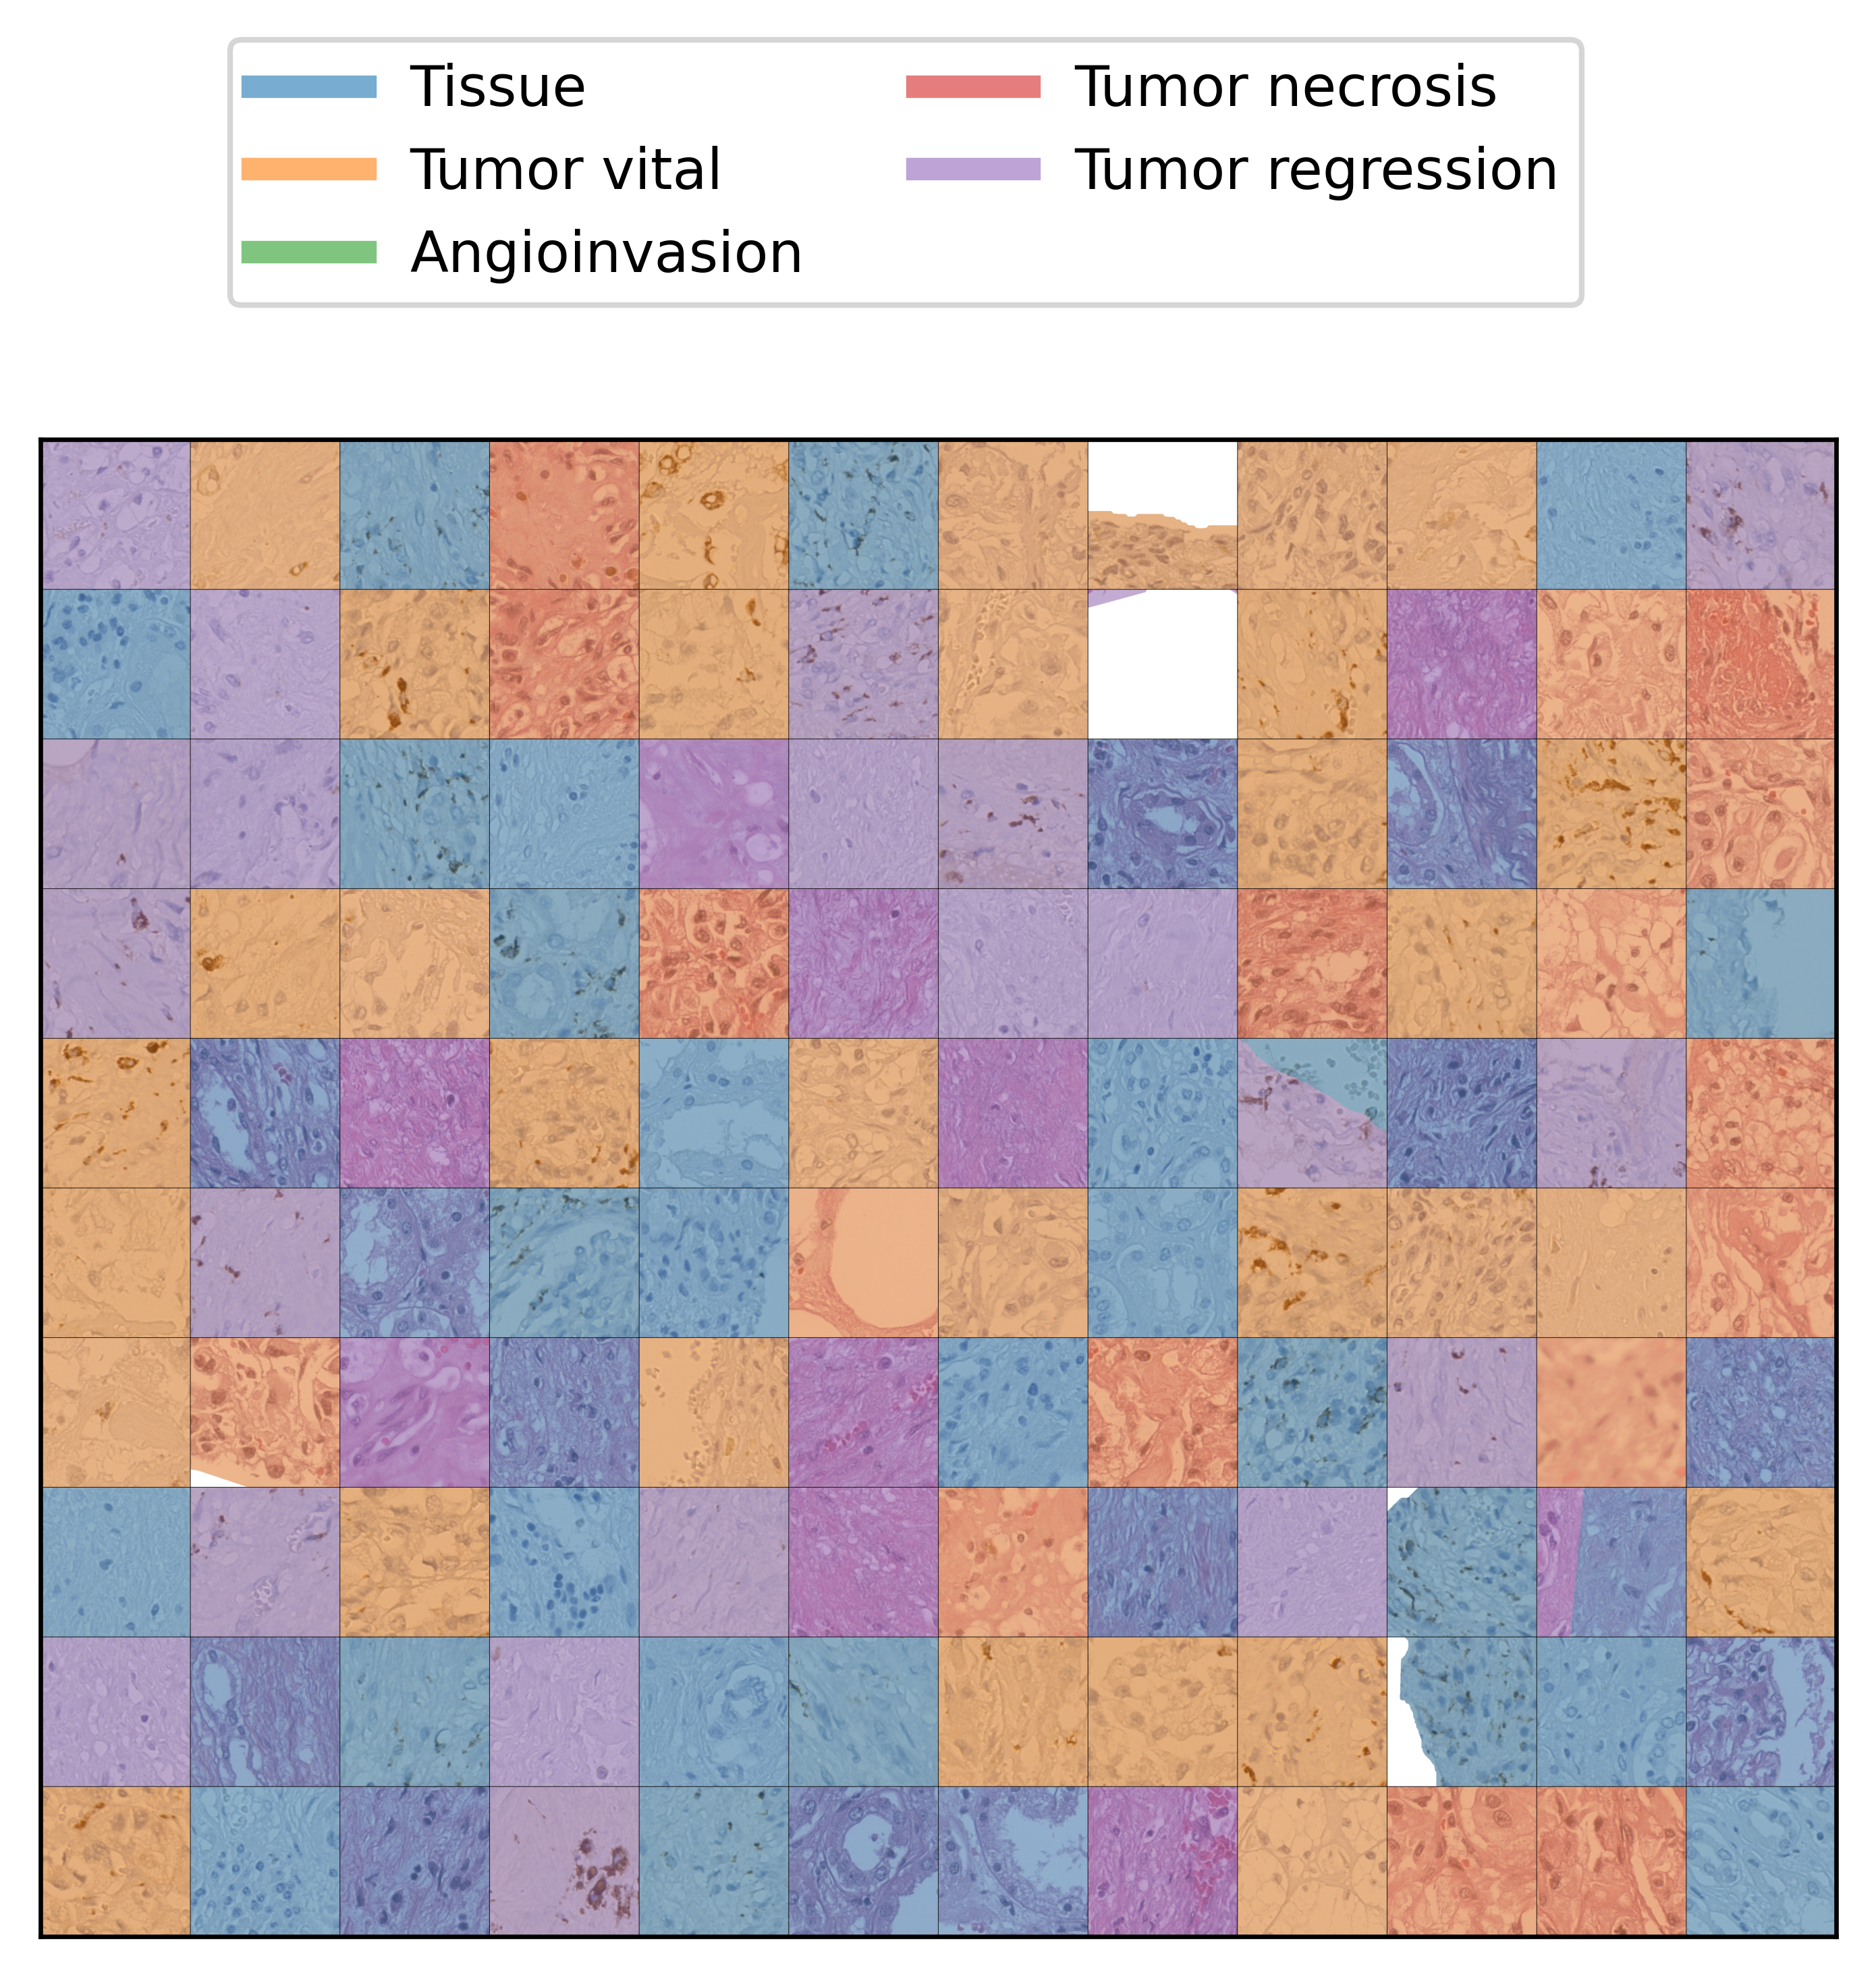
\includegraphics[width=0.75\textwidth]{latex/figures/postproc_subimage_1_(120, 12).png}
    \caption[Patch extraction]{Random selection of extracted patches with the corresponding mask overlaid in colour. White areas are not part of the tissue, but the empty background. Each patch has dimensions of 512x512 pixels and is extracted from a WSI with each dimension being at least close to 100,000 pixels.}
    \label{fig:patches}
\end{figure}

\subsection{Downsampled WSIs}
    \label{DownsampleData}
As mentioned above, an alternative approach to dividing images into patches is to load them at reduced resolution and size. Although fine-grained information is lost, this way, the spatial information can be maintained easily. Also, no bias is created, unlike random sampling of patches does. Moreover, this is computationally inexpensive, as each SVS file already contains versions of its image at lower resolutions. The general approach works as follows:

In a small preprocessing step, each tissue mask is loaded at the desired resolution to determine the respective maximum width and height of the tissue within the whole image. This is necessary because of the varying dimensions of each image. Also, due to quality issues of the scans, there are WSIs with a lot of whitespace. As a WSI scanner produces an WSI by scanning tiles on a grid, it usually skips tiles that do not contain tissue by checking an area of the glass slide at a higher resolution. The final output is then truncated to not contain large areas without tiles that were actually scanned. However, if such a tile contains contaminations such as dust, water droplets, etc. it will be scanned and the WSI cannot be truncated properly any more. Hence, the location of the tissue (top-right coordinate) to be used for later extraction of only relevant regions is stored as well. 
Fortunately, this pre-processing has to be done only once, since the representation of each sample can simply be stored according to JavaScript object notation (JSON). The created JSON file is an array of objects (a list of dictionaries in Python) where each object contains the paths to its SVS file and the corresponding masks in TIFF format. Furthermore, each record stores relevant metadata, such as the case ID, the stain code, the coordinate from where the tissue is to be extracted and the aforementioned maximum width and height over the entire data set. This has the advantage that the representation can be easily updated in \(O(k)\) where \(k\) is the number of new samples, rather than in \(O(n)\) where \(n\) represents the final size of the data set. Especially if the maxima remain the same, since existing records do not need to be updated at all. This approach allows to later load only the area of an image that actually contains tissue. Thus, it speeds up repetitive loading of images and masks during training without requiring significant amounts of extra storage. 

In the presented experiments, each WSI is read at level 3 which corresponds to a downsampling factor of 64. The images are padded equally on each side with zeroes until they equal the dimensions of the respective maxima determined earlier. There might be a shift towards the bottom or right by one pixel, which is the case if a completely even padding is not possible due to the respective dimensions of the image itself. This approach was chosen over simply resizing them to prevent a possible loss of information. Since all images are taken at the same magnification by the scanner, resizing them could distort the spatial information as objects get enlarged. Figure \ref{fig:downsample_input} visualises the input received by the neural network. The first three channels represent the image data in RGB format and are shown as a single image here. Stacked on top are the different masks in a pre-defined order.

\begin{figure}[h!t]
    \centering
    % \vspace{-14pt}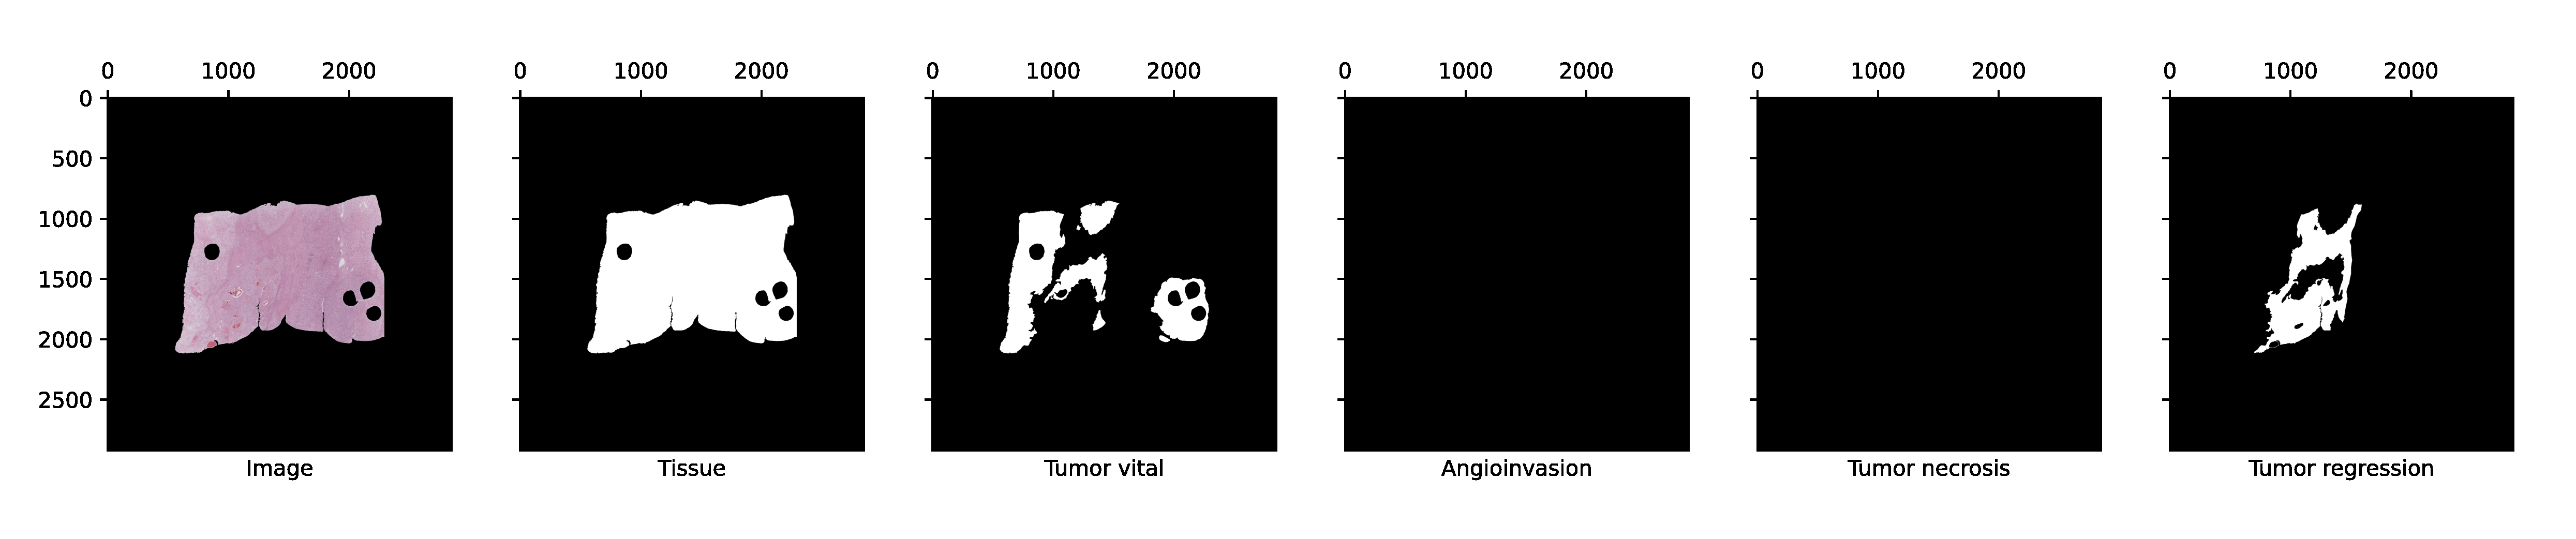
\includegraphics[width=\textwidth,trim={0 0 0 40pt},clip]{latex/tissue/AAA_postproc_subimage_1-1.png} \\
    \vspace{-14pt}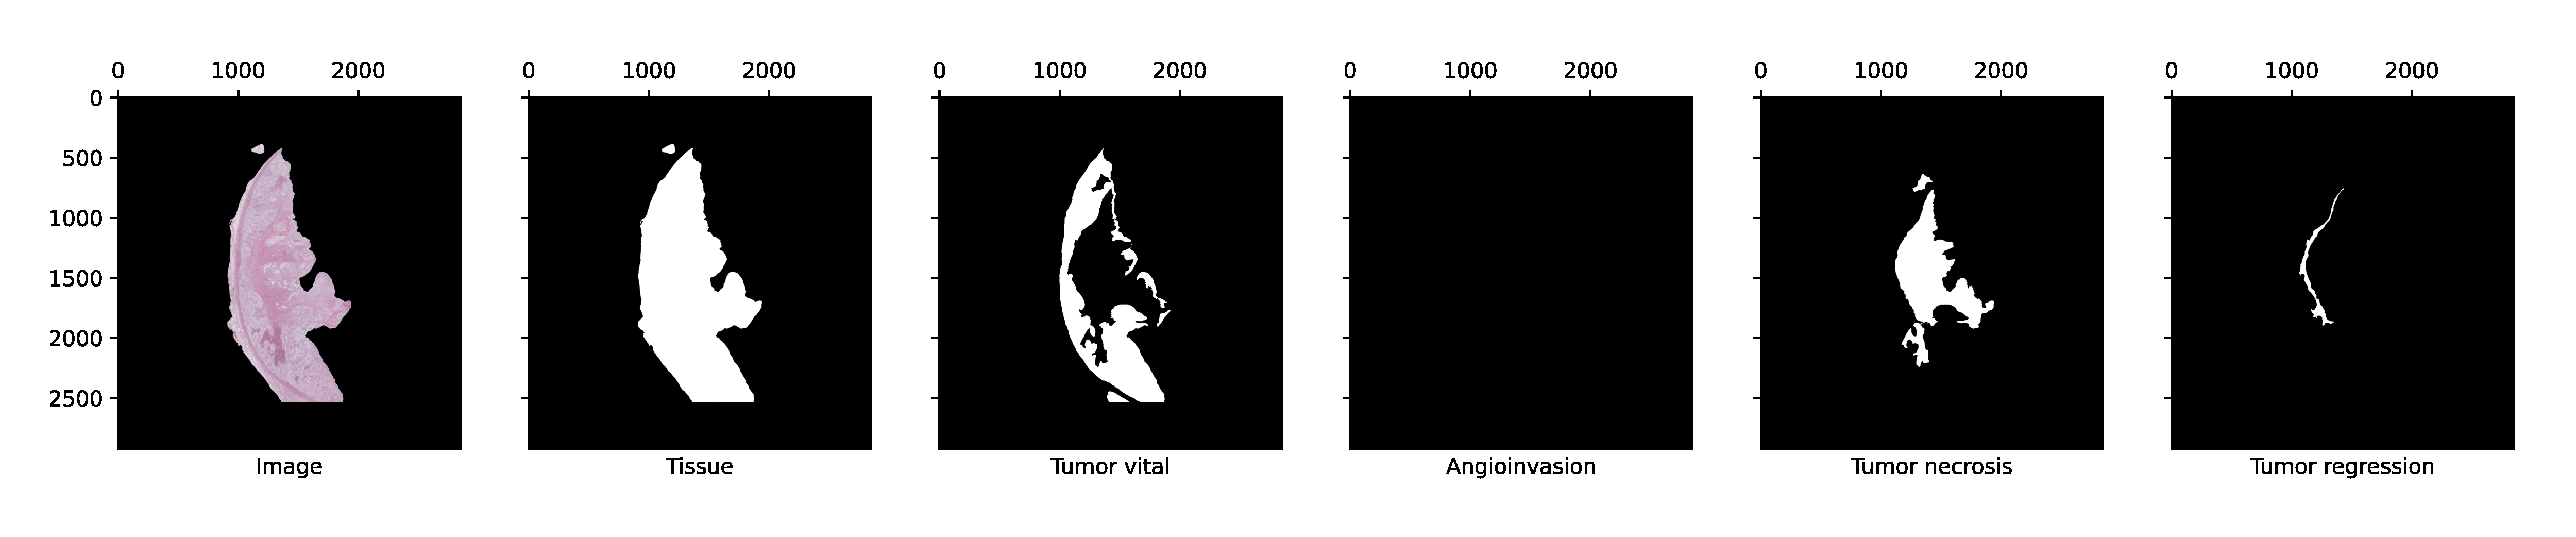
\includegraphics[width=\textwidth,trim={0 0 0 20pt},clip]{latex/tissue/AAA_postproc_subimage_3-1.png} \\
    \vspace{-14pt}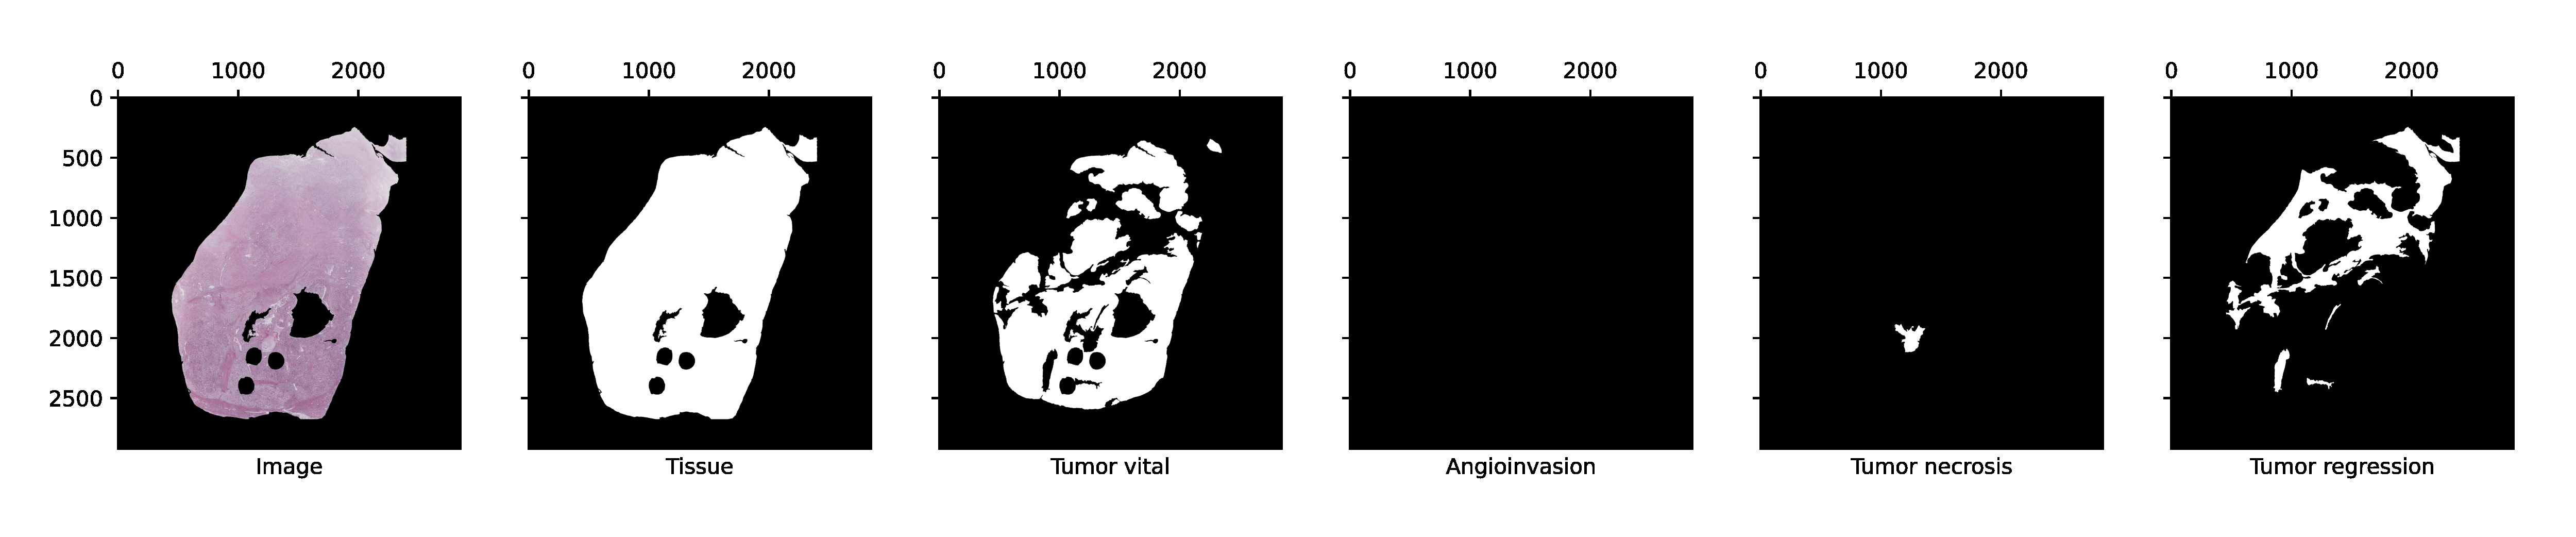
\includegraphics[width=\textwidth,trim={0 0 0 40pt},clip]{latex/tissue/AAA_postproc_subimage_12-1.png} \\ 
    \vspace{-14pt}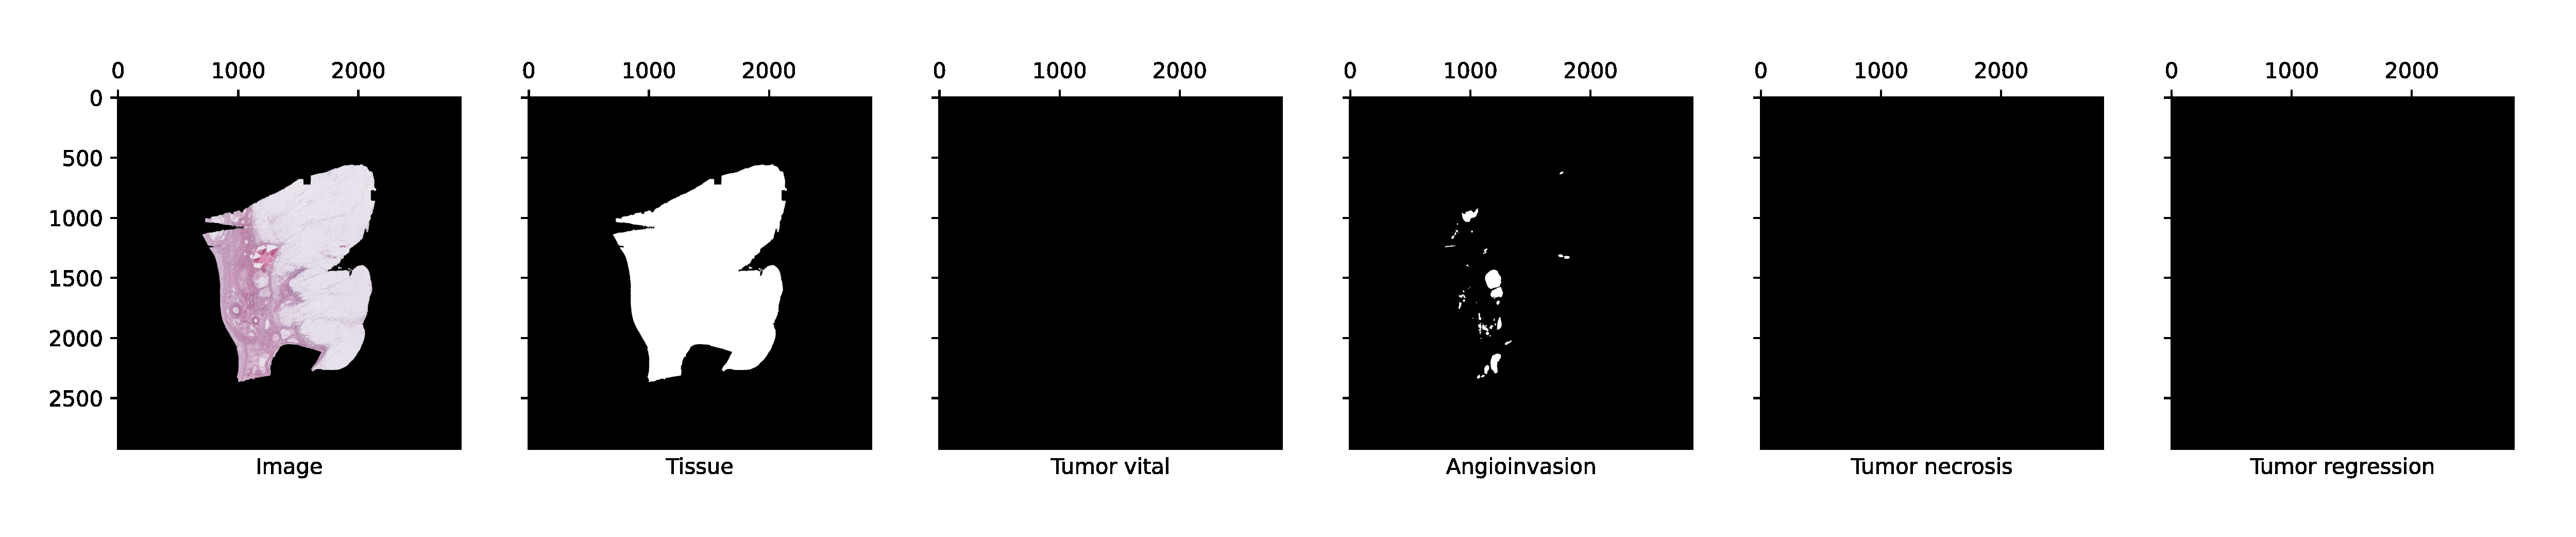
\includegraphics[width=\textwidth,trim={0 0 0 40pt},clip]{latex/tissue/AAA_postproc_subimage_19-1.png} \\
    \vspace{-14pt}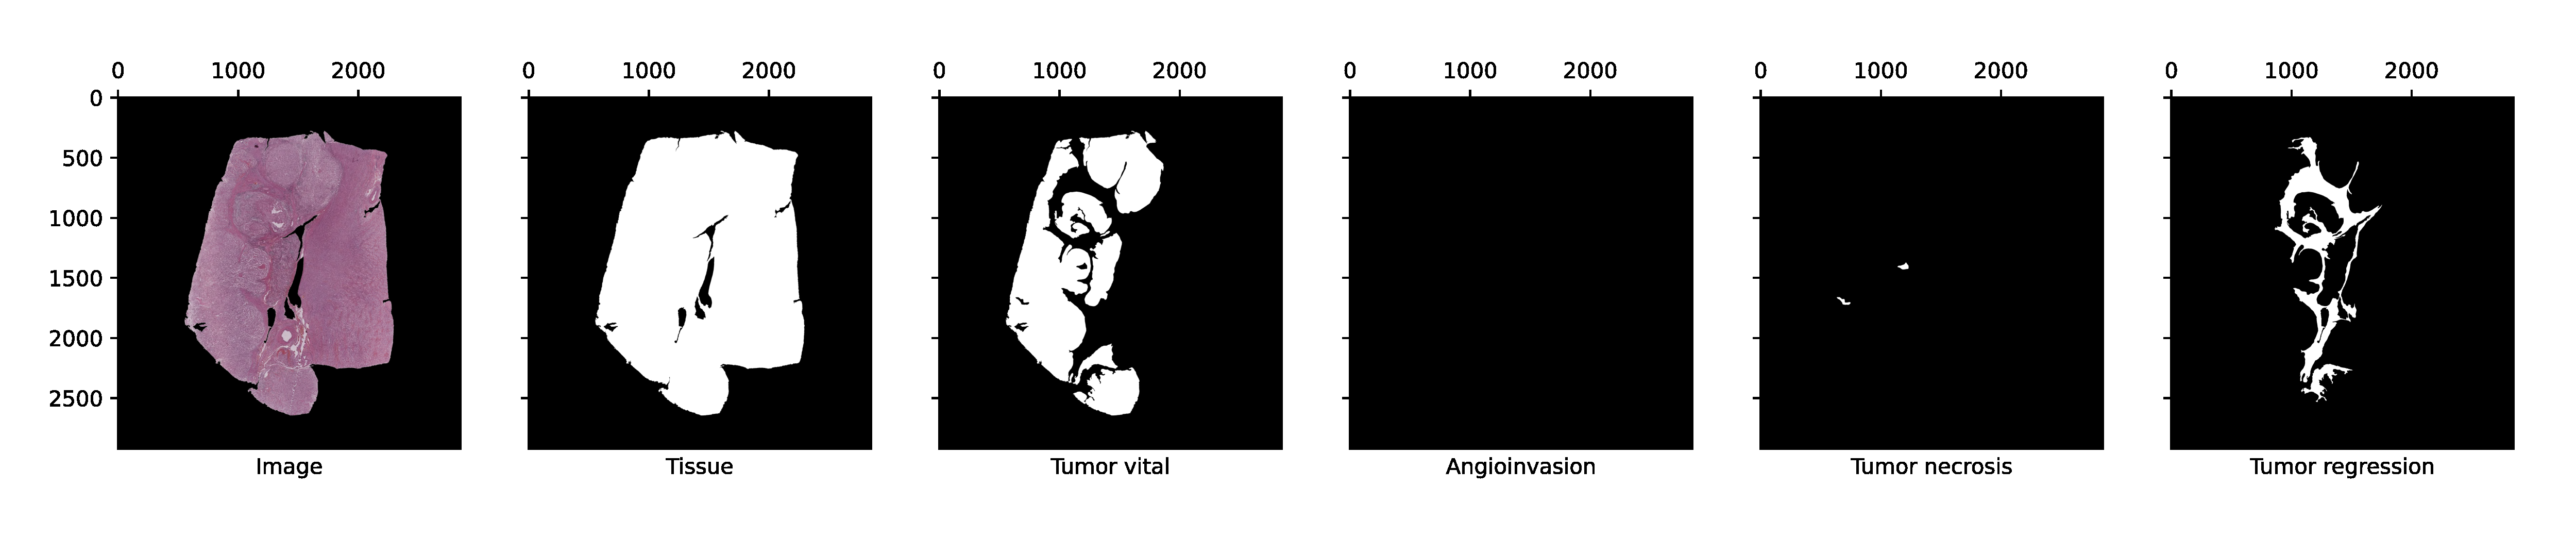
\includegraphics[width=\textwidth,trim={0 0 0 40pt},clip]{latex/tissue/AAA_postproc_subimage_158-1.png} \\
  \caption[Neural network input]{Representation of the input to the neural network. The “image” represents a tensor of dimensions CxHxW where C is 3. Each mask is a 2D tensor. All are stacked into a single 3D Tensor with 8 channel dimensions. Both axes represent the coordinates in pixels. Shown are the cases with IDs 1, 3, 12, 19 and 158 from top to bottom.}
  \label{fig:downsample_input}
\end{figure}

\subsection{Data Augmentation}

We use random transformations to augment the dataset and thus induce better generalization. For this purpose, the inputs are randomly flipped on both axes. This is applied to both the images themselves and the accompanying masks, independent of them being patches or downsampled slides. By this approach, we hope to prevent the network from overfitting on the shape of the objects presented. Especially since each patient contributes multiple samples that are similar in their high-level appearance, this is a possible risk.
Also, the WSIs brightness, contrast, and saturation are jittered by a small value. This is done to create minor variations between samples in addition to the larger ones already present. This helps to increase the generalization performance of the model, which is to be preferred over a higher score on the current dataset. The literature does support this approach, as it is common that scanners and stains do not produce not perfectly reproducible results. Hence, it makes sense to mimic this behaviour artificially. \cite{Macenko2009method, Ciompi2017importance}

\section{Network Architectures}
  \label{NetArch}

\subsection{WSI networks}

\subsubsection{ResNet} First, a ResNet-based CNN was used to analyse only all slides in a unimodal way. For this purpose, the implementation \verb | resnet101 | of the Python package \verb|torchvision| was chosen. The choice for a ResNet based architecture is rooted in the results of the chamelyon17 challenge, where this architecture was employed frequently with good results. \cite{Bandi2019Detection} Although, this challenge was carried out on a different task using different evaluation methods, we hypothesise that these findings are still applicable to our problem. Since CNN architectures are used as a means to extract features, i.e., to identify repeating higher-level structures in the image, the benefit to survival analysis can be expected to be similar.

However, these ResNet models expect an image in the RGB (Red-Green-Blue) colour space, i.e. the input is expected to be a 3-dimensional tensor with 3 channels in the outer dimension. Hence, a single convolutional layer was placed in front of the ResNet model to reduce the input dimensionality accordingly. This layer is accompanied by dropout and the rectified linear unit (ReLU) activation function, analogous to the original input layer of the ResNet architecture. 
These two conventional convolutional layers are followed by 4 residual blocks, each consisting of convolution, dropout, and batch norm layers followed by the ReLU activation function. The prediction of sample-specific risks was performed in two ways. First, by a single fully connected layer, thus transforming the 1000 input nodes into a single output value. In the second approach, the convolutional layers are followed by two fully connected (FC) layers. The first FC layer facilitates the learning of correlations between input to the hidden nodes. The second layer performs the prediction by outputting a single value. In the multimodal setting, the output of the first FC layer is fused with the other modalities and then processed by more FC layers. This potentially enables each modality to be first analysed separately and to look for within-modality interactions before considering cross-modality interactions as well. An illustration of these architectures can be found in the appendix \ref{fig:network_archs}. 
Due to memory requirements of our approach, only a batch size of 3 could be realised. This has the consequence that gradient accumulation was necessary to allow meaningful steps against the gradient. With this technique, multiple gradients are computed, and a step is taken on the average of these gradients only after a certain number of such iterations. Optimising over gradients that were computed with small amounts of samples increases the risk of inefficient steps which do not move the weights towards the minima of the true gradient of the full dataset. This is especially the case, if this small subset is not representative for the full dataset and can in turn slow down convergence significantly. Therefore, an initial accumulation factor of 12 was chosen, resulting in an effective batch size of 36. While a higher amount of accumulations might stabilise the training prices even further, it increasingly slows down training as well.
\subsubsection{EfficientNet} 
Besides ResNet, EfficientNetV2 was tested for image analysis of the WSIs. The \verb|torchvision| implementation \verb|efficientnet_v2_s| of EfficientNetV2 was used. Analogous to our ResNet approach, a preliminary convolutional block, modelled after the input layers of \verb|efficientnet_v2_s| reduces the number of channels of the input. 
The last convolutional layer of the model was replaced in order to be able to alter the size of the feature vector. A single linear layer was used for the prediction of hazards.
\subsubsection{Distributed Training} 
All training that involved the WSI data was carried out using the distributed data parallel paradigm, as implemented in the Python package \verb|PyTorch|. With this method, the dataset is divided among multiple GPUs and then processed in parallel. The weights and gradients are synchronised before and after each optimisation step. This allows us to increase the effective batch size by the number of GPUs deployed. Interestingly, the synchronisation overhead is reduced thanks to the accumulation of gradients that we perform. As synchronisation is only necessary during actual weight adjustments, the frequency of synchronisations is reduced. The more advanced paradigm Fully Sharded Data Parallel (FSDP) was also trialled, but no improvement in processing speed was observed. Meanwhile, the performance of the network itself remained identical under deterministic conditions. 
For actual training, the data was divided into splits of 75\%, 15\% and 5\% for training, validation and test sets, respectively. For the purpose of overfitting on 5\% of the data, a 50/50 split was performed between the training and validation set. This change was necessary, because the validation set would have contained too few uncensored samples otherwise. Hence, the subset of the data set consisted of 35 samples.
\subsubsection{Overfitting} 
Overfitting can be helpful in evaluating the capabilities of a model. It is desirable that a model is able to overfit on a small dataset, since that usually ensures that it contains sufficient complexity to represent the data. However, this must be regarded with some scepticism. Since the subset of data is chosen randomly, it is not guaranteed to represent the entire dataset or its complexity. This means that the model might not be able to overfit the full dataset but only the small subset of it, which defeats the purpose of these experiments. However, for the case of tissue slides, it is unlikely that some samples are drastically more or less complex than the other samples. For example, if we were to use a heterogenous dataset consisting of multiple cancer types or subtypes, this would be a more serious concern. 
Another issue are the binary masks, which are stacked on top of each WSI. Since only a few samples contain annotations for “Angioinvasion” or “Tumour Necrosis”, there is a high chance that WSIs with such annotations are not adequately represented. That is because these samples are scarce and their area is quite small if they are present. Therefore, the more concerning question would be whether something is learnt from these annotations at all.

\subsection{Processing Genomic Data}

Analogue to the WSI data, the gene count data from the NanoString assay was also analysed in isolation. For this, the Self normalizing network architecture previously employed by Chen et al. in PathomicFusion \cite{Chen2022Pathomic} was adapted. This network consists of four self-normalising layers. These types of layers were first proposed by Klambauer et al.\cite{Klambauer2017Self} Each layer consists of a fully connected layer, the scaled exponential linear unit (SeLU) as the activation function, and an Alpha dropout layer. These layers drive each output towards zero mean and unit variance; these properties are then maintained by Alpha Dropout. This strategy has been shown to prevent instabilities caused by vanishing or explosive gradients. \cite{Chen2022Pathomic}
These self normalising subnetwork is followed by a single fully connected layer that performs the prediction. In contrast to PathomicFusion, our network uses SeLU activation functions instead of Exponential Linear Units (ELU). For the purpose of training the neural network, each feature was standardised across samples using the \verb|StandardScaler| class from the Python package \verb|scikit-learn|. Figure \ref{fig:SNN} shows a visualisation of that network.

\begin{figure}[h!t]
    \centering
    \includegraphics[width=\textwidth]{latex/networks/genomic_snn.onnx_horz.png}
    \caption[Self Normalizing Network Diagram]{Self Normalizing network for NanoString Gene Expression data. The network consists of 4 blocks. Each is made up of a fully connected Layer (FC), Alpha Dropout (ADP) and a scaled exponential linear unit (SeLU). Lastly another fully connected layer performs the prediction. This figure was created using the Netron web tool. \cite{Roeder2023Netron}}
    \label{fig:SNN}
\end{figure}

\subsection{Fusion Network}

As our tests included some more involved methods, others are more straightforward. This section will explain each of them, starting with the strategies belonging to the latter category.

\subsubsection{Vector based fusion methods} 
These methods all consist of simple vector operations. For once, we take the element-wise sum of the feature vectors, hence using a single vector of the same size as the unimodal ones as input to the network. In the same manner, the element-wise product and the element-wise maximum of features are tested as well. However, by concatenating the unimodal feature representations, the last of these simple approaches does change the shape of the input to the prediction network. We deal with the doubled length by adjusting the input size of the following fully connected layer accordingly.

\subsubsection{EmbraceNet} The EmbraceNet \cite{Choi2019EmbraceNet} approach was already briefly mentioned in chapter \ref{related}. We apply only the fusion part of EmbraceNet, i.e. the embracement layers as a fusion technique. We do not require the use of docking layers, as we train the subnetworks of our end-to-end model to learn feature representations of the same dimensionality. This fusion approach is based on probabilities, where each position of the input vectors is assigned a probability that decides from which input vectors the respective value should be taken. If a modality is missing, their probabilities are set to zero. For our bimodal approach, that means that the input is treated as unimodal for cases where the genomic data is missing. Despite that, all modalities present have equal probabilities of being picked for an element of the output vector otherwise.

\subsubsection{Kronecker-based fusion} For this approach, we adopted the PathomicFusion methodology proposed by Chen et al. Our implementation is very closely modelled after their bimodal fusion method. In this approach, the learnt feature representations are fused by computing the Kronecker product, which is the outer product between all the unimodal vectors. For the bimodal approach, this means that the input are two 1D vectors of the same size, one for the WSI data and the other for the genomic data. The output then is a 2D matrix with dimensions equal to the length of each vector. However, there is a preliminary step that aims to improve the results. In order to reduce the impact of noisy unimodal features, a gating-based attention mechanism is placed between the unimodal networks and the fusion mechanism. With this mechanism, we learn the importance of each feature in each unimodal vector with respect to the other modalities. The softmax probabilities of the resulting attention weights are applied to each unimodal representation. Afterwards, the vectors are fused as described above. \cite{Chen2022Pathomic} Due to the size of our feature vectors, we had to downsample using bilinear transformations.  Hence, a four times smaller representation had to be created before Kronecker fusion could be applied.   

\subsubsection{Attention} This approach employs a simple attention layer to produce attention weights for each unimodal feature vector. This is done with a single fully connected layer where the input size is equal to the output size, and no bias term is used. This layer is combined with the hyperbolic tangent activation function, followed by a softmax operation. During backpropagation, the weights of this layer are trained to be directly interpretable as feature importance weights. Each attention vector is then applied to its respective feature vector by element-wise multiplication. Afterwards, the sum of the attended feature vectors is taken in order to receive a 1D input for prediction. However, in this approach, missing modalities are factored in by scaling up the values of the fused vector, where the values are multiplied by the count of empty modalities.

\section{Experimental exploration}

% \subsection{Hardware}

The unimodal SNNs were trained on a single NVIDIA GeForce RTX 3060 Ti GPU. Both the unimodal WSI networks and the fusion networks were trained on 4 NVIDIA A40 GPUs using Distributed Data Parallel and \verb|pytorch|. Before we could train the network with the settings as described in chapter \ref{Results}, various tests were necessary. For once, we tried to train the image network with WSI at the larger levels (4x, 16x) first, only to find that that was not feasible. Furthermore, multiple different approaches for efficient handling of the data were explored as well. 

A copy of the code is available at the department of Data Science in Biomedicine at the Peter L. Reichertz Institute for Medical Informatics (PLRI) and an updated version will also be publicly be available in the foreseeable future at \url{github.com/seapat/renal-cancer-dl}.


% The first attempt was to train on a downsampled resolution. This was a seemingly easy approach, since, thanks to the pyramidal tiff files, images at lower resolutions were already available. That being said, there are many issues with this Approach, all stemming from memory limitations. Firstly, loading images at the first downsampling resolution (4x) was not possible, as a single sample did not fit into memory. 
% At the second level (16x), a mini-batch with a size of two is possible. However, this causes problems for a considerable subset of samples. Since the loss ignores censored samples, there is a risk that both samples are censored, and a sensual negative log-likelihood cannot be computed. Gradient accumulation helps with this

% \subsection{Nanostring data}

% We run comparisons to determine the impact of different hyperparameters by modifying a single one while leaving all other hyperparameters fixed. We chose to first adjust the learning rate to find the most promising one. From that starting point, we compared different dropout probabilities and different lengths for the feature vector that serves as input either to the prediction in the unimodal case, or for the  multimodal fusion. For the first comparison, the same dropout  rate was applied to all layers. We tested values 0.1, 0.25 and 0.5. For the second comparison, four different sizes were evaluated. Namely, vectors of length 250, 500, 750 and 1000 were returned. 

% \section{Interpretability Methods}

% All employed methods for model interpretability were implemented using the Python packages \verb|captum|. The Saliency, Input X Gradient, Integrated Gradients and GradCAM algorithms were used to gain insights on the feature attribution of the image data. For this purpose, the best-performing unimodal model trained on the WSI data was used. For each method, the 
% %TODO: specify outlier_perc, ie number of extremes that were ignored.
\cleardoublepage

%%
%%%%%%%%%%%%%%%%%%%%%%%%%%%%%%%%%%%%%%%%%%%%%%%%%%%%%%%%%%%%%%%%%%%%
% Diskussion und Ausblick
%%%%%%%%%%%%%%%%%%%%%%%%%%%%%%%%%%%%%%%%%%%%%%%%%%%%%%%%%%%%%%%%%%%%

\chapter{Results}
  \label{Results}

\section{WSI networks}

\ref{fig:1FCmodel} shows the results of the ResNet-based model, with only one fully connected layer following the residual blocks. In \ref{fig:1fc_overfit}, the model was run on a small subset ($n=35)$ of the full dataset, to verify the capabilities of the model. \ref{fig:1fc_normal} shows the training results on the full dataset. Both experiments were run for 500 epochs and each took around 15 hours to finish.  
When comparing the loss curves, we notice that the training and validation loss starts to diverge around epoch 75 in figure \ref{fig:1fc_overfit} but not in figure \ref{fig:1fc_normal}. Additionally, we notice that in both cases the validation loss stays above the training loss, with the training loss reaching similar values of 0.14 and 0.13 for full and reduced dataset respectively. Also notable is, that the initial losses are identical when training on the whole dataset but different on the subset intended for overfitting the model.
The achieved concordance indices are indicated in table \ref{tab:c_indices}

\begin{table}[hb!]
    \centering
    \caption{Latest recorded concordance indices for experiments related to unimodal WSI data.}
    \begin{tabular}{l | c c}
       Experiment & Training & Validation  \\ [0.5ex] 
       \hline  
        1 FCL Overfit & 0.93 & 0.78 \\ 
        1 FCL Normal & 0.86 & 0.89 \\
        2 FCL lr 0.01 & 0.86 & 0.89 \\
        2 FCL lr 0.001 & 0.84 & 0.78 \\
        EfficientNet & 0.82 & 0.93 \\
        \hline
    \end{tabular}
    \label{tab:c_indices}
\end{table}


\begin{figure}[h!t]
    \centering
     \begin{subfigure}[b]{0.495\textwidth}
         \centering
         \includegraphics[width=\textwidth]{latex/loss_plots/!!!_overfit0.05.png}
         \caption{Overfitting on subset of data}
         \label{fig:1fc_overfit}
     \end{subfigure}
    \hfill
     \begin{subfigure}[b]{0.495\textwidth}
         \centering
         \includegraphics[width=\textwidth]{latex/loss_plots/!!!_2023-04-03.png}
         \caption{Training on whole dataset}
         \label{fig:1fc_normal}
     \end{subfigure}
    \hfill
    \caption[CNN with Single-Layer Prediction]{Results of ResNet based CNN using a single fully connected output layer. Figure \ref{fig:1fc_overfit} shows the results of overfitting the network on 5\% of data (n=35). Figure \ref{fig:1fc_normal} shows the results for training on the full dataset.}
    \label{fig:1FCmodel}
\end{figure}

The experiment was repeated with the ResNet architecture replaced with a model that was based on EfficientNetV2 \cite{Tan2021EfficientNetV2}. Figure \ref{fig:Effnet} contains the corresponding results. We notice that the concordance index for the validation set overtakes the one for the training set at around 100 epochs, due to a steeper ascend until that point. 

\begin{figure}[h!t]
    \centering
     \begin{subfigure}[b]{0.495\textwidth}
         \centering
         \includegraphics[width=\textwidth]{latex/loss_plots/acc12_lr0.01_effnets.png}
         \caption{Training and validation loss}
         \label{fig:effnetloss}
     \end{subfigure}
    \hfill
     \begin{subfigure}[b]{0.495\textwidth}
         \centering
         \includegraphics[width=\textwidth]{latex/ci_plots/acc12_lr0.01_effnets.png}
         \caption{Concordance indices}
         \label{fig:effnetci}
     \end{subfigure}
    \hfill
    \caption[EfficientNet with Single-Layer Prediction]{EfficientNet implementation trained on WSI data.}
    \label{fig:Effnet}
\end{figure}


Figure \ref{fig:resnet_lr} shows the second version of our ResNet model, which was later used for the fusion approaches. We tested the model with two different learning rates. When using a learning rate of 0.001, we again notice a divergence of losses after some time. Also, in both settings, the validation loss tracks the training loss very close for a few epochs, after which it diverges. Most notable is the difference in concordance indices, where the learning rate of 0.01 leads to higher values consistently. 
As we considered gradient accumulations necessary to be able to retrieve reliable results despite low batch sizes per iteration, we also experimented with different numbers of accumulation steps. This experiment was conducted at a learning rate of 0.01 and hence is best compared to the previous experiment at the same learning rate since only the number of accumulations differ. We see almost identical results, only the concordance index of the validation data seems to converge faster with less accumulation steps.

\begin{figure}[h!t]
    \centering
 \begin{subfigure}[b]{0.49\textwidth}
     \centering
     \includegraphics[width=\textwidth]{latex/loss_plots/2FC_lr_0.01.png}
     \caption{Losses at lr 1e-2 and 12 gradient accumulations}
 \end{subfigure}
    \hfill
     \begin{subfigure}[b]{0.49\textwidth}
         \centering
         \includegraphics[width=\textwidth]{latex/ci_plots/2FC_lr_0.01.png}
         \caption{Concordance indices at lr 1e-2 and 12 gradient accumulations}
     \end{subfigure}
\vskip\baselineskip
     \begin{subfigure}[b]{0.49\textwidth}
         \centering
         \includegraphics[width=\textwidth]{latex/loss_plots/2FC_lr_0.001.png}
         \caption{Losses at lr 1e-3}
     \end{subfigure}
    \hfill
     \begin{subfigure}[b]{0.49\textwidth}
         \centering
         \includegraphics[width=\textwidth]{latex/ci_plots/2FC_lr_0.001.png}
         \caption{Concordance indices at lr 1e-3}
     \end{subfigure}
    \hfill
     \begin{subfigure}[b]{0.49\textwidth}
     \centering
     \includegraphics[width=\textwidth]{latex/loss_plots/24accums.png}
     \caption{Losses at 24 gradient accumulations}
    \end{subfigure}
    \hfill
     \begin{subfigure}[b]{0.49\textwidth}
         \centering
         \includegraphics[width=\textwidth]{latex/ci_plots/24accums.png}
         \caption{CI at 24 gradient accumualtions}
     \end{subfigure}
    \hfill
    \caption[Resnet with Double-Layer Prediction ]{ResNet implementation using two fully connected layers for hazard prediction. Comparison of different learning rates (lr) and different number of iterations before an optimisation step.}
    \label{fig:resnet_lr}
\end{figure}

\clearpage

\section{Gene expression data}

\subsection{Quality Control}

Figure \ref{fig:RCCQC} shows the results of the quality controls for the gene expression data. The presented controls were first conducted by NanoString, but then repeated due to concerns regarding quality of the provided data. 
\subsubsection{Binding Density} The binding density of the probes within the imaging area is shown in figure \ref{fig:BindDens} as the concentrations of barcodes per lane. Samples are shown as green dots, and panel standards are shown as green triangles. There are two samples per lane, as two cartridges were used for the experiment. The lower and upper thresholds for passing the control are situated at 0.5 and 2.5 respectively and visualised as grey dashed lines. Most samples have a binding density below that of the standards (at a binding density of about 0.9). The only exception is one sample in lane 7 and both samples from lane 12. All samples pass the control, with the samples in lane 1 barely above the minimum threshold. \cite{Gorman2022IO, NanoStringTechnologies2017Gene}
\subsubsection{Limit of Detection} The limit of detection is shown in figure \ref{fig:LOD}. It represents a comparison of positive and negative controls. The counts of the negative controls are seen as box plots, each having a mean count below 16. The positive control \verb|Pos_E| has a concentration of 0.5 fM. It is required to be at least two standard deviations higher in terms of counts. This threshold is shown as a red horizontal line for each sample, respectively. All samples pass this control as well. Also, all samples have more counts than the panel standards. \cite{Gorman2022IO, NanoStringTechnologies2017Gene}
\subsubsection{Positive Linearity Control} The results of the positive linearity control are illustrated in figure \ref{fig:PosLin}. It shows the positive controls and the panel standards, which have different target concentrations. Corresponding data points are connected by edges. The correlation after $Log_2$ transformation between the known concentrations of positive controls and the observed counts is shown. Correlations below 0.95 may indicate problems. However, all samples pass this control as well. \cite{Gorman2022IO, NanoStringTechnologies2017Gene}

\begin{figure}[h!t]
    \centering
 \begin{subfigure}[b]{0.475\textwidth}
     \centering
     \includegraphics[width=\textwidth]{latex/figures/NanostringBindingDensity.png}
     \caption{Binding Density}
     \label{fig:BindDens}
 \end{subfigure}
    \hfill
     \begin{subfigure}[b]{0.475\textwidth}
         \centering
         \includegraphics[width=\textwidth]{latex/figures/PositiveLimitOfDetection.png}
         \caption{Limit of Detection}
         \label{fig:LOD}
     \end{subfigure}
    \vskip\baselineskip
     \begin{subfigure}[b]{0.475\textwidth}
         \centering
         \includegraphics[width=\textwidth]{latex/figures/PositiveLinearity.png}
         \caption{Positive Linearity}
         \label{fig:PosLin}
     \end{subfigure}
    \hfill
    \caption[NanoString Quality Control]{Visualisations of Quality Control metrics. Figure \ref{fig:BindDens} shows the binding density of each sample respective to their lane as green dots. Dashed grey lines show the respective upper and lower thresholds, while green triangles represent the panel standards for comparison. Figure \ref{fig:LOD} shows the limit of detection as counts per sample and of the panel standards. The box plots correspond to the negative controls. Red horizontal lines represent the threshold each sample has to pass. Figure \ref{fig:PosLin} shows the positive control linearity. For each sample, the counts of the respective positive controls and the panel standards are shown against the concentration in femtomolar (fM). 
    Each sample passes all quality controls. Each figure were taken from the automated report conducted by NanoString \cite{Gorman2022IO}} 
    \label{fig:RCCQC}
\end{figure}


\subsection{Baseline model}

A Baseline model was fitted to the subcohort of 24 samples for which gene expression data was available. This model achieved a concordance index of $0.98$ and $1.0$ on train and test data, respectively.
Figure \ref{fig:SurvRaceSmall} gives an overview over the available data. Of 24 patients, 14 are censored, leaving 10 patients with recorded survival times. Most uncensored patients showed a relatively short survival time, with patient 151 being a notable exception. An identical Figure for the whole cohort can be found in the appendix (Figure \ref{fig:SurvRaceFull}).
For each of the 750 cancer-relevant genes, the model did calculate the hazard ratios (HR) as log-transformed coefficients. Figure \ref{fig:HRGenes} shows the subset of genes with $log(\text{HR})$ of less than $0.99$ or more than $1.01$. These genes have a particularly positive or negative effect on patient survival.
Figure \ref{fig:DevianceResiduals} visualises the deviance residuals of patients and their survival times. Except for one value, all samples are situated in the range of $[-1,1]$. Censored and uncensored patients are marked blue and orange, respectively.

\begin{figure}[h!t]
    \centering

     \begin{subfigure}[b]{0.49\textwidth}
         \centering
         \includegraphics[width=\textwidth]{latex/figures/impactful_genes_hazard_ratio.png}
         \caption{Features with HR $\ge 1.01$ or $\le 0.99$}
         \label{fig:HRGenes}
     \end{subfigure}
    \hfill
     \begin{subfigure}[b]{0.49\textwidth}
         \centering
         \includegraphics[width=\textwidth]{latex/figures/deviance_residuals_rcc.png}
         \caption{Deviance Residuals}
         \label{fig:DevianceResiduals}
     \end{subfigure}

    \hfill
    \caption[Baseline model on genomic data]{
    Figure \ref{fig:HRGenes} shows genes with notable hazard ratios (HR) and their respective error bars.
    Figure \ref{fig:DevianceResiduals} shows the deviance residuals per patient over their survival times. Censoring status is marked as orange or blue if the patient died or got censored, respectively.}
    \label{fig:BaselineModel}
\end{figure}

\subsection{Self normalising Neural networks}

Figures \ref{fig:snn_dropout} and \ref{fig:snn_fsz} show the hyperparameter search experiments for the SNN trained on gene expression data. After a preliminary search for a suitable learning rate, with the result being \(1e-5\), we explored different dropout probabilities as well as output sizes for the feature extraction part of the network. Due to strong fluctuations in values between consecutive epochs, exponential moving averaging was applied to all results with a window size of 30. 

Figure \ref{fig:snn_dropout} shows the result for varying probabilities for randomly dropping single nodes in each hidden layer. We note that both the concordance index and the loss stagnate with a dropout ratio of 0.5. The only exception is the validation loss, where a steady rise is observed. Generally, when looking at the metrics during training, we can observe that a lower dropout probability results in a more convex loss and CI over time. 
When inspecting the validation data, we notice that the loss increases until a certain plateau is hit, after which it decreases for some epochs before it starts to rise again. Meanwhile, a lower value for $p$ seems to help the CI rise earlier for the validation set. However, there does not seem to be a notable difference for the final (smoothed) values.

\begin{figure}[h!t]
    \centering
 \begin{subfigure}[b]{0.49\textwidth}
     \centering
     \includegraphics[width=\textwidth]{latex/loss_plots/snn_dropout_train.png}
     \caption{Training loss}
 \end{subfigure}
    \hfill
     \begin{subfigure}[b]{0.49\textwidth}
         \centering
         \includegraphics[width=\textwidth]{latex/loss_plots/snn_dropout_val.png}
         \caption{Validation loss}
     \end{subfigure}
\vskip\baselineskip
     \begin{subfigure}[b]{0.49\textwidth}
         \centering
         \includegraphics[width=\textwidth]{latex/ci_plots/snn_dropout_train_ci.png}
         \caption{Training concordance index}
     \end{subfigure}
    \hfill
     \begin{subfigure}[b]{0.49\textwidth}
         \centering
         \includegraphics[width=\textwidth]{latex/ci_plots/snn_dropout_val_ci.png}
         \caption{Validation concordance index}
     \end{subfigure}
    \hfill
    \caption[Experiments on dropout probability for SNN]{Experiments on dropout probability for SNN. All parameters of the network stayed the same, except for the probability parameter of each alpha dropout layer in the network. All models were trained for the same duration on the same hardware. Each curve was smoothed using exponential moving averages with a window of 30 samples.}
    \label{fig:snn_dropout}
\end{figure}

Figure \ref{fig:snn_fsz} illustrates the behaviour of the metrics dependent on the output size in the last hidden layer. We tested four different values by incrementing them by 250 for each experiment. For both the training loss and the training CI, the values differ barely over time. Towards the end of each experiment, the losses are diverging, while the CI values are converging. The differences are less nuanced for the validation dataset. A feature size of 750 resulted in the highest loss over the whole duration of the experiment. The other tested sizes show similar values for the most time until the last 200 epochs, where the smallest size results in the lowest final loss. Generally, the same behaviour as in the experiments related to the dropout rate can be observed. First the loss increases, then a local minimum is found which is left towards the end of the training time. 
The concordance indices for the validation data reflect the inverse results of the loss curves. The lowest feature size achieves the highest CI, while the opposite is the case for the feature size of 750.

\begin{figure}[h!t]
    \centering
 \begin{subfigure}[b]{0.49\textwidth}
     \centering
     \includegraphics[width=\textwidth]{latex/loss_plots/snn_fsz_train.png}
     \caption{Training loss}
 \end{subfigure}
    \hfill
     \begin{subfigure}[b]{0.49\textwidth}
         \centering  
         \includegraphics[width=\textwidth]{latex/ci_plots/snn_fsz_train_ci.png}
         \caption{Training concordance index}
     \end{subfigure}
\vskip\baselineskip
     \begin{subfigure}[b]{0.49\textwidth}
         \centering
         \includegraphics[width=\textwidth]{latex/loss_plots/snn_fsz_val.png}
         \caption{Validation loss}
     \end{subfigure}
    \hfill
     \begin{subfigure}[b]{0.49\textwidth}
         \centering
         \includegraphics[width=\textwidth]{latex/ci_plots/snn_fsz_val_ci.png}
         \caption{Validation concordance index}
     \end{subfigure}
    \hfill
    \caption[Experiments on feature size for SNN]{Experiments on feature size for SNN. All parameters of the network stayed the same, except for the output size parameter of the second last fully connected layer of the network. All models were trained for the same duration on the same hardware. Each curve was smoothed using exponential moving averages with a window of 30 samples.}
    \label{fig:snn_fsz}
\end{figure}

As mentioned above, the SNN was trained at different learning rates, for which the results can be seen in figure \ref{fig:snn_lr_loss}. Additionally, the model was also evaluated with the amount of hidden layers reduced to one. 
We observe that, if only using one hidden layer, the local minimum is reached much earlier than in the experiments in \ref{fig:snn_fsz}. However, it rises in the same manner while the training loss is steadily decreasing. Altering the learning rate by one decimal position impacts the loss dramatically. We notice that the maximum validation loss reached is higher the lower the learning rate is. Furthermore, the rise is also much steeper. In all cases, the validation loss eventually increases while the training loss decreases. What differentiates the experiments is the time point when this starts occurring and the speed at which it happens.
These experiments were run for 2500 epochs to better understand the long term development of the loss. The corresponding CI curves can be found in the appendix in figure \ref{fig:snn_lr_ci}

\begin{figure}[h!t]
    \centering
 \begin{subfigure}[b]{0.49\textwidth}
     \centering
     \includegraphics[width=\textwidth]{latex/loss_plots/SNNet_fsz250_1Layer.png}
     \caption{SNN with single hidden layer}
 \end{subfigure}
    \hfill
     \begin{subfigure}[b]{0.49\textwidth}
         \centering
         \includegraphics[width=\textwidth]{latex/loss_plots/SNNet_fsz250_1e-4_2500epochs.png}
         \caption{SNN at lr 1e-4}
     \end{subfigure}
\vskip\baselineskip
     \begin{subfigure}[b]{0.49\textwidth}
         \centering
         \includegraphics[width=\textwidth]{latex/loss_plots/SNNet_fsz250_1e-5_2500epochs.png}
         \caption{SNN at lr 1e-5}
     \end{subfigure}
    \hfill
     \begin{subfigure}[b]{0.49\textwidth}
         \centering
         \includegraphics[width=\textwidth]{latex/loss_plots/SNNet_fsz250_1e-6_2500epochs.png}
         \caption{SNN at lr 1e-6}
     \end{subfigure}
    \hfill
    \caption[SNN with varying learning rates and models]{Experiments for SNN on learning rates and number of hidden dimensions. Neither x-axis nor y-axis are uniform.}
    \label{fig:snn_lr_loss}
\end{figure}

The final model that was decided upon, uses a dropout rate of 0.25, a learning rate of 1e-5 and its last hidden layer produces a vector of size 1000. This model is used in the following section for building the fusion models.

\clearpage

\section{Fusion comparison}

Due to concerns regarding the required time, each fusion experiment was run for only 300 epochs. We assume that this should be enough to determine the most promising fusion technique, which can then be used for further optimisations. Each experiment still required at least 9 hours of time to complete.
Figures \ref{fig:fusions_simple} and \ref{fig:fusions_complex} shows the result of the six different approaches that have been tested. Except of the particular fusion mechanic, all parameters were the same. From table \ref{tab:c_indices_fuse} and the figures, we can observe that the approaches there are indeed notable differences. Especially, the Kronecker approach seems to stagnate over the course of training. 
The training losses are higher on average since their calculation is cumulative and the size of the respective dataset is larger. Hence, comparisons of different losses within a dataset are more appropriate than between the datasets. 
It should also be noted that the metrics in Table \ref{tab:c_indices_fuse} correspond to the latest model, after the last epoch, rather than the best performing one. As the presented results only serve as an indication of the particular learning progress of the model, it is more reasonable to compare them at the same time point. Each model would be needed to be trained to convergence first before an evaluation of the best possible performance is reasonable. 

\begin{table}[h!b]
    \centering
    \caption[Fusion networks metrics]{Concordance Indices and negative log likelihoods of different fusion approaches. Losses to the left, and concordance indices to the right.}
    \begin{tabular}{l | c c c | c c c }
         \hline
        \multirow{2}{*}{} & \multicolumn{3}{c|}{Concordance index} & \multicolumn{3}{c}{Likelihood Loss} \\ [0.5ex]
        \hline
       Experiment & Training & Validation & Test & Training & Validation & Test \\ [0.5ex]
       \hline  
        Maximum        & 0.594 & 0.590 & 0.618  & 2.025 & 0.648 & 0.532 \\
        Summation      & 0.637 & 0.651 & 0.566  & 1.643 & 0.681 & 0.703 \\
        Concatenated  & 0.709 & 0.522 & 0.589  & 2.148 & 1.611 & 0.616 \\
        EmbraceNet     & 0.596 & 0.644 & 0.486  & 1.041 & 0.706 & 0.752 \\
        Attention      & 0.492 & 0.500 & 0.549  & 1.319 & 0.652 & 0.558 \\
        Kronecker      & 0.580 & 0.594 & 0.612  & 1.117 & 0.570 & 0.570 \\
        \hline
    \end{tabular}
    \label{tab:c_indices_fuse}
\end{table}


\begin{figure}[h!b]
    \centering
     \begin{subfigure}[b]{\textwidth}
         \centering
         \includegraphics[width=0.49\textwidth]{latex/loss_plots/max.png}
         \includegraphics[width=0.49\textwidth]{latex/ci_plots/max.png}
         \caption{Element-wise maximum}
     \end{subfigure}
\vskip\baselineskip
     \begin{subfigure}[b]{\textwidth}
         \centering
         \includegraphics[width=0.49\textwidth]{latex/loss_plots/cat.png}
         \includegraphics[width=0.49\textwidth]{latex/ci_plots/cat.png}
         \caption{Concatenation}
     \end{subfigure}
\vskip\baselineskip
     \begin{subfigure}[b]{\textwidth}
         \centering
         \includegraphics[width=0.49\textwidth]{latex/loss_plots/sum.png}
         \includegraphics[width=0.49\textwidth]{latex/ci_plots/sum.png}
         \caption{Element-wise summation}
     \end{subfigure}
    \hfill
    \caption[Vector-based Fusion techniques]{Straightforward fusion techniques, that consist of a single vector-vector operation. Losses to the left, and concordance indices to the right.}
    \label{fig:fusions_simple}
\end{figure}

% \clearpage

\begin{figure}[h!b]
        \centering
     \begin{subfigure}[b]{\textwidth}
         \centering
         \includegraphics[width=0.49\textwidth]{latex/loss_plots/attention.png}
         \includegraphics[width=0.49\textwidth]{latex/ci_plots/attention.png}
         \caption{Attention-based}
     \end{subfigure}

\vskip\baselineskip
     \begin{subfigure}[b]{\textwidth}
         \centering
         \includegraphics[width=0.49\textwidth]{latex/loss_plots/embrace.png}
         \includegraphics[width=0.49\textwidth]{latex/ci_plots/embrace.png}
         \caption{EmbraceNet}
     \end{subfigure}

\vskip\baselineskip
     \begin{subfigure}[b]{\textwidth}
         \centering
         \includegraphics[width=0.49\textwidth]{latex/loss_plots/kronecker.png}
         \includegraphics[width=0.49\textwidth]{latex/ci_plots/kronecker.png}
         \caption{Attention-gated Kronecker product}
     \end{subfigure}

    \hfill
    \caption[Complex Fusion techniques]{Complex fusion techniques that involve either stochastic processes or additional hidden layers.}
    \label{fig:fusions_complex}
\end{figure}

%%%%%%%%%%%%%%%%%%%%%%%%%%%%%%%%%%%%%%%%%%%%%%%%%%%%%%%%%%%%%%%%%%%%%%%%%%%%%%%%%%%%%%%%%%%%%%%%%%%%%%%%%%%%%
\clearpage

\section{Interpretability}

The ResNet version of the unimodal model for processing the WSI was used to analyse the feature attribution of the WSI images. Examples of the corresponding results are shown in figures \ref{fig:case111a}, \ref{fig:case111b}, \ref{fig:case13a}, \ref{fig:case13b}, \ref{fig:case13c}, and \ref{fig:case129}. The attributions of the Guided GradCAM method were not converted to absolute values, because the rescaling of values to fit the colour scale would have made interesting aspects appear invisible. 
Integrated Gradients were calculated using 50 intermediate steps. For GradCAM, the last convolutional layer was used to calculate the attribution. As the convolutional layer has much smaller dimensions than the original input image, the results were expected to be more coarse, as can be seen in the figure. 
The occlusion technique uses a kernel of size 8×50×50 with stride of 8×50×50 as well. Saliency and Input*Gradient have no adjustable parameters to be reported. 

All the cases shown here were part of the test set during training. This means that these samples were not used for training nor model evaluation during training. The model used for inference was picked from the training epoch with the highest concordance index on the validation set.

\ref{fig:case129} shows only a selection of applied method, as some results were deemed less interesting. More visualisation in the same manner can be found in Appendix \ref{chap:App2} Figures \ref{fig:case181} and \ref{fig:case121}.

\begin{figure}[h!t]
    \centering
     \begin{subfigure}[b]{0.475\textwidth}
         \centering
         \includegraphics[width=\textwidth]{latex/captum/case111/masks_case111-stain1-censored_3499days.png}
         \caption{Tumour annotations of WSI}
     \end{subfigure}
    \hfill
     \begin{subfigure}[b]{0.49\textwidth}
         \centering
         \includegraphics[width=\textwidth]{latex/captum/case111/integrated_gradients_abs_case111-stain1-censored_3499days.png}
         \caption{Integrated Gradients, abs. attributions}
     \end{subfigure}
\vskip\baselineskip
     \begin{subfigure}[b]{0.49\textwidth}
         \centering
         \includegraphics[width=\textwidth]{latex/captum/case111/guided_gradcam_pos_case111-stain1-censored_3499days.png}
         \caption{Guided GradCAM, positive attributions}
     \end{subfigure}
    \hfill
     \begin{subfigure}[b]{0.49\textwidth}
         \centering
         \includegraphics[width=\textwidth]{latex/captum/case111/guided_gradcam_neg_case111-stain1-censored_3499days.png}
         \caption{Guided GradCAM, negative attributions}
     \end{subfigure}
    \hfill
    \caption[Integrated gradients and Guided GradCAM for case 111]{Results of Integrated Gradients and Guided GradCAM for case 111. The figure of the tumour masks is included for comparison. Integrated Gradients attributions are converted to absolute values.}
    \label{fig:case111a}
\end{figure}


\begin{figure}[h!t]
    \centering
     \begin{subfigure}[b]{0.475\textwidth}
         \centering
         \includegraphics[width=\textwidth]{latex/captum/case111/masks_case111-stain1-censored_3499days.png}
         \caption{Tumour annotations of WSI}
     \end{subfigure}
    \hfill
     \begin{subfigure}[b]{0.49\textwidth}
         \centering
         \includegraphics[width=\textwidth]{latex/captum/case111/Occlusion_abs_case111-stain1-censored_3499days.png}
         \caption{Occlusion map; kernel and stride of 50}
     \end{subfigure}
\vskip\baselineskip
     \begin{subfigure}[b]{0.49\textwidth}
         \centering
         \includegraphics[width=\textwidth]{latex/captum/case111/saliency_case111-stain1-censored_3499days.png}
         \caption{Saliency Maps}
     \end{subfigure}
    \hfill
     \begin{subfigure}[b]{0.49\textwidth}
         \centering
         \includegraphics[width=\textwidth]{latex/captum/case111/inputXgradient_pos_case111-stain1-censored_3499days.png}
         \caption{Input*Gradient}
     \end{subfigure}
  
    \hfill
    \caption[Occlusion and Saliency for case 111]{Results of Saliency, Input*Gradients and occlusion mapping for case 111. The figure of the tumour masks is included for comparison. All attributions were converted to absolute values.}
    \label{fig:case111b}
\end{figure}


\begin{figure}[h!t]
    \centering
     \begin{subfigure}[b]{0.475\textwidth}
         \centering
         \includegraphics[width=\textwidth]{latex/captum/case13/masks_case13-stain41-dead_2415days.png}
         \caption{Tumour annotations of WSI}
     \end{subfigure}
    \hfill
     \begin{subfigure}[b]{0.49\textwidth}
         \centering
         \includegraphics[width=\textwidth]{latex/captum/case13/integrated_gradients_abs_case13-stain41-dead_2415days.png}
         \caption{Integrated Gradients, abs. attributions}
     \end{subfigure}
\vskip\baselineskip
     \begin{subfigure}[b]{0.49\textwidth}
         \centering
         \includegraphics[width=\textwidth]{latex/captum/case13/guided_gradcam_pos_case13-stain41-dead_2415days.png}
         \caption{Guided GradCAM, positive attributions}
     \end{subfigure}
    \hfill
     \begin{subfigure}[b]{0.49\textwidth}
         \centering
         \includegraphics[width=\textwidth]{latex/captum/case13/guided_gradcam_neg_case13-stain41-dead_2415days.png}
         \caption{Guided GradCAM, negative attributions}
     \end{subfigure}
    \hfill
    \caption[Integrated gradients and Guided GradCAM for case 13  stain 41]{Results of Integrated Gradients and Guided GradCAM for case 13  stained for CD8 and CD20. The figure of the tumour masks is included for comparison. Integrated Gradients attributions are converted to absolute values.}
    \label{fig:case13a}
\end{figure}


\begin{figure}[h!t]
    \centering
     \begin{subfigure}[b]{0.475\textwidth}
         \centering
         \includegraphics[width=\textwidth]{latex/captum/case13/masks_case13-stain41-dead_2415days.png}
         \caption{Tumour annotations of WSI}
     \end{subfigure}
    \hfill
     \begin{subfigure}[b]{0.49\textwidth}
         \centering
         \includegraphics[width=\textwidth]{latex/captum/case13/Occlusion_abs_case13-stain41-dead_2415days.png}
         \caption{Occlusion map; kernel and stride of 50}
     \end{subfigure}
\vskip\baselineskip
     \begin{subfigure}[b]{0.49\textwidth}
         \centering
         \includegraphics[width=\textwidth]{latex/captum/case13/saliency_case13-stain41-dead_2415days.png}
         \caption{Saliency Maps}
     \end{subfigure}
    \hfill
     \begin{subfigure}[b]{0.49\textwidth}
         \centering
         \includegraphics[width=\textwidth]{latex/captum/case13/inputXgradient_pos_case13-stain41-dead_2415days.png}
         \caption{Input*Gradient}
     \end{subfigure}
  
    \hfill
    \caption[Occlusion and Saliency for case 13  stain 41]{Results of Saliency, Input*Gradients and occlusion mapping for case 13. The figure of the tumour masks is included for comparison. All attributions were converted to absolute values.}
    \label{fig:case13b}
\end{figure}

\begin{figure}[h!t]
    \centering
     \begin{subfigure}[b]{0.475\textwidth}
         \centering
         \includegraphics[width=\textwidth]{latex/captum/case13b/masks_case13-stain42-dead_2415days.png}
         \caption{Tumour annotations of WSI}
     \end{subfigure}
    \hfill
     \begin{subfigure}[b]{0.49\textwidth}
         \centering
         \includegraphics[width=\textwidth]{latex/captum/case13b/integrated_gradients_abs_case13-stain42-dead_2415days.png}
         \caption{Integrated Gradients, abs. attributions}
     \end{subfigure}
\vskip\baselineskip
     \begin{subfigure}[b]{0.49\textwidth}
         \centering
         \includegraphics[width=\textwidth]{latex/captum/case13b/guided_gradcam_pos_case13-stain42-dead_2415days.png}
         \caption{Guided GradCAM, positive attributions}
     \end{subfigure}
    \hfill
     \begin{subfigure}[b]{0.49\textwidth}
         \centering
         \includegraphics[width=\textwidth]{latex/captum/case13b/saliency_case13-stain42-dead_2415days.png}
         \caption{Saliency Map, abs. attributions}
     \end{subfigure}
    \hfill
    \caption[Integrated gradients, Guided GradCAM and saliency for case 13 stain 42]{Results of Integrated Gradients and Guided GradCAM for case 13 stained for CD4 and FoxP3. The figure of the tumour masks is included for comparison. Integrated Gradients attributions are converted to absolute values.}
    \label{fig:case13c}
\end{figure}


\begin{figure}[h!t]
    \centering
     \begin{subfigure}[b]{0.475\textwidth}
         \centering
         \includegraphics[width=\textwidth]{latex/captum/case129/masks_case129-stain19-dead_414days.png}
         \caption{Tumour annotations of WSI}
     \end{subfigure}
    \hfill
     \begin{subfigure}[b]{0.49\textwidth}
         \centering
         \includegraphics[width=\textwidth]{latex/captum/case129/integrated_gradients_abs_case129-stain19-dead_414days.png}
         \caption{Integrated Gradients, abs. attributions}
     \end{subfigure}
\vskip\baselineskip
     \begin{subfigure}[b]{0.49\textwidth}
         \centering
         \includegraphics[width=\textwidth]{latex/captum/case129/guided_gradcam_pos_case129-stain19-dead_414days.png}
         \caption{Guided GradCAM, positive attributions}
     \end{subfigure}
    \hfill
     \begin{subfigure}[b]{0.49\textwidth}
         \centering
         \includegraphics[width=\textwidth]{latex/captum/case129/saliency_case129-stain19-dead_414days.png}
         \caption{Saliency Map, abs. attributions}
     \end{subfigure}
    \hfill
    \caption[Integrated gradients, Guided GradCAM and saliency for case 129 stain 19]{Results of Integrated Gradients and Guided GradCAM for case 129 stained for CD204. The figure of the tumour masks is included for comparison. Integrated Gradients and saliency attributions are converted to absolute values.}
    \label{fig:case129}
\end{figure}

% 001 = HE-Elastika
% 016 = CD68 (Makrophagen)
% 019 = CD204 (TAM)
% 041 = CD8_CD20
% 042 = CD4_FoxP3

\cleardoublepage

%%
%%%%%%%%%%%%%%%%%%%%%%%%%%%%%%%%%%%%%%%%%%%%%%%%%%%%%%%%%%%%%%%%%%%%
% Diskussion und Ausblick
%%%%%%%%%%%%%%%%%%%%%%%%%%%%%%%%%%%%%%%%%%%%%%%%%%%%%%%%%%%%%%%%%%%%

\chapter{Discussion and Outlook}
  \label{Discussion}
  
\section{Findings}

\subsection{Single layer predictions on WSIs}

In Figure \ref{fig:1FCmodel} we see an evaluation of the expressive power of our model. On the reduced dataset, we clearly see that the model is unable to generalise well to the validation data. Although, the model does not achieve a validation loss similar to the training one, we see a clear improvement when utilizing the whole dataset. However, interesting is the behaviour in the first 50 epochs of training. In both plots, we notice an initial decrease in loss over the first 50 epochs. In figure \ref{fig:1fc_normal}, the validation loss perfectly tracks the training loss. In the overfitting experiment, we see an initial learning of the model. In general, this behaviour is to be expected, as the model has not started to 'memorise' the training data yet. However, this could be further facilitated due to the structure of the dataset and because of how the split into training and validation set is performed. Although each WSI is a different slide and also stained differently, a single patient contributes multiple images. Because of that, these images often share a similar shape. Since, we do not control whether images from one patient end up in both the training and the validation set, this could affect the performance of the network. As the network is learning with the training data, it might optimise for the corresponding images in the validation set. With that being said, we do not believe that this is the sole or the most significant contributor to the networks' performance. If that were the case, we would expect it to perform even better on the validation set, especially on the reduced dataset. If the data in the validation set were too similar, we would not be able to induce overfitting. Furthermore, we see that the overfitting stops together with the convergence of the training as expected.

\subsection{Unimodal Networks}

\subsubsection{EfficientNet versus ResNet} As seen in the results section, although the original version of EfficientNet managed to outperform ResNet, ours did not. While the concordance index might be higher on the validation set, it is not for the training data and neither are the losses better than the ResNet model. This raises the question which metric is the most relevant one and which one we should optimise for. Liao \textit{et al.} argue that a combination of characteristics should be considered. \cite{Liao2022Empirical} Hence, we decided to conduct consecutive experiments using the ResNet based approach. In the following paragraph, we discuss possible reasons for the differences in performance.
For once, we applied the exact same hyperparameters as in our most successful experiment of ResNet (learning rate 0.01, 12 gradient accumulations). Obviously, what works well with ResNet does not necessarily work well for other models. To better compare both, we would need to evaluate EfficientNet with different hyperparameters, like we did with the ResNet model. In favour of other experiments and the main aim of this work, we did not follow through on this endeavour. 
This brings us to another suitable aspect for optimisation. We modified both ResNet and EfficientNet, but not in the same manner. While we add two fully connected layers, one for feature extraction and the other for prediction, we only add one for EfficientNet and modify the last convolutional layer instead. Hence, the fully connected feature extraction and prediction happens both in the last layer simultaneously. While we could not find a significant difference in performance between using one or two fully connected layers in ResNet, this could very well be the case for EfficientNet. Furthermore, EfficientNet has less learnable parameters, but the overall number of layers is higher. As this network architecture has been thoroughly optimised for a completely different task, that being classification on small images, it might simply not be suited for our aims. Perhaps the fact that the ResNet architecture did not undergo such tunings is the reason it performs better. An interesting observation shown in figure \ref{fig:Effnet} is that towards the end of the training period, the training loss seems to be catching up with that of ResNet. It would have been interesting to see how this development behaves at later epochs. However, the authors claim that their network also converges faster, \cite{Tan2021EfficientNetV2} a finding that we could not confirm. Despite that, the training speed was indeed faster. While each ResNet experiment required about 15 hours to process the 500 epochs, the EfficientNet experiments concluded around 3 hours earlier.
The initial idea behind using EfficientNetV2 was the promise to better handle large input images. ResNet is trained to use images of 224x224 pixels, but our input is multiple magnitudes larger. Due to the average pooling layers both ResNet and EfficientNet employ, this does not pose an issue from an implementation perspective, but could very well degrade prediction performance. As the largest variant of EfficientNetV2 is designed and pre-trained for inputs of size 480x480 pixels, we assume that it would be better suited for our data, since this increases the level of detail that is directly put into the network. However, using the larger version was not possible due to the memory limitations of the hardware. The small version of EfficientNetV2 uses an input size of 384 pixels along width and height, which is still more than ResNet. But that did yield a benefit in the end.
Concluding this analysis, probably a proper hyperparameter hyper and model optimization is needed to gain useful insights on the cause of the divergence of expectation and result. 

\subsubsection{ResNet: learning rate and gradient accumulations}

We explored the effect that alterations of single hyperparameters have on the performance of the neural network. First, we lowered the learning rate by one decimal position from 0.01 to 0.001. The results of this can be seen in \ref{fig:resnet_lr}. As we can see, a lower learning rate leads to a worse concordance index and a worse overall loss. Furthermore, we see that the generalisation on the validation set is worse. The CI at \(lr=0.001\) is lower than the one for the training dataset, while the opposite is the case at \(lr=0.01\). Usually, there are two reasons why a model performs better on the validation data than on the training data. For once, we disable regularisation techniques such as dropout during validation. Doing the same for training data would also produce better results. Furthermore, the validation is always run after the full iteration on the training dataset. Hence, the full learning progress during an epoch is already reflected at validation time but can only be observed on the next epoch for the training dataset. 

Also interesting is the development of training and validation losses. We can see that at around 200 epochs, the validation loss starts stagnating for the lower learning rate. At the higher learning rate, the descent only slows down, parallel to the training loss. Hence, we see a clear divergence with the lower learning rate, which means that the generalisation of the model is getting worse, as the training loss keeps decreasing. 
What raises questions is the stagnation of the validation loss. Normally, one would expect that lower learning rates lead to a slower convergence speed, and thus are only necessary if a minimum would be overstepped otherwise. A possible reason for the validation loss may be that the parameters of the network are “stuck” at a local minimum, which the model cannot “leave” because of the small learning rate. In such cases, a higher learning rate helps to escape local minima or to avoid entering them in the first place.
The fact that the increase in accumulations does not have a meaningful effect is less surprising. Since we use a batch size of 3 and train the network using Distributed Data Parallel on 4 GPUs, we end up at an effective batch size of 144 already, which is roughly 20.4\% of our dataset. Perhaps, this is already enough information to make reasonable weight adjustments and doubling this number (effectively) does not yield a worthwhile benefit.

\subsubsection{SNN: Gene expression networks}

We see in figures \ref{fig:snn_fsz} that the number of learned features does only slightly impact the training loss, while the differences are more noticeable on the validation set. The same is true for the corresponding concordance indices. 

The effect of the dropout probability is more noticeable, as can be seen in figure \ref{fig:snn_dropout}. With a probability of 0.5, hence there is a 50\% chance that nodes are set to zero during training, the loss stays unchanged except for a short decrease in the very early epochs. On the validation set, this leads to a steady increase over time without any signs of convergence. Decreasing the probability also decreases the lowest training loss achieved within 1000 epochs. For the validation set, a probability of 0.25 leads to loss first increasing, but after around 500 epochs it plateaus briefly, after which it declines. However, as in all experiments, the loss starts to increase again towards the end of the training time. With a probability of 0.1 the early increase is way less noticeable; however, the same increase sets in earlier, at around 600 epochs, and is much steeper. That means that the network is overfitting earlier and stronger.
The concordance indices both reach high values of above 0.9, with the \(p=0.1\) leading to an almost perfect score. Furthermore, the lower the dropout rate, the faster the convergence of the CI. Even at a rate of 0.5, the CI is slowly increasing. The dropout rate seems to have less impact on the final CI, under the condition that it is low enough to facilitate learning on the training set.

However, one thing is common to all experiments. Towards the end of the training period, the validation loss increases. Hence, all models start overfitting eventually, and none of the parameters we altered seem to change that. By performing a full and extensive hyperparameter search, perhaps a setting can be found for which the model does not overfit. However, we already show that the model stops learning at all if regularisation is too high. Hence, if such a window exists, it is very small. In comparison, we were able to show that a simple linear model manages to adjust almost perfectly, at least as far as the concordance index is concerned. As deep neural networks are known to be more data hungry than conventional machine learning methods, another conclusion becomes apparent. That is, that we simply do not have enough data samples to train a complex “big data” model that generalises well on unseen data. 
However, we also show that our approach is feasible, as our model manage to reach a concordance index of almost 1.0 with the right hyperparameters. This is further supported by our findings in figure \ref{fig:snn_lr_loss}. A simpler model, with only one layer, produces worse results in the sense that the minimum loss is higher, and the overfitting starts sooner. This is the case due to our use of regularisation techniques (self-normalisation) with each layer, and hence the overall regularisation is stronger by adding more layers. We hypothesise that more available data would allow significant simplifications of the SNN model. Furthermore, we show that a learning rate of 0.00001 is necessary. Increasing it leads to a dramatic acceleration of the rise of the validation loss. Meanwhile, lowering the learning rate slows down the progress to the point that improvement in metrics is barely observable. This supports our theory that the window of optimal parameters, where no overfitting occurs, is very narrow, if it exists at all. 

\subsection{Fusion networks}

The different fusion experiments were run as described in section \ref{MetMat}. Furthermore, we used a learning rate of 0.01 and 0.00001 for the WSI and gene expression networks, respectively. As we could show that these parameters work well in the respective unimodal settings, we assume them to be good starting points for the fusion network as well. The learning rate for the remaining layers, which were the fusion layers, if applicable, and the prediction layers, was set to 0.001. The fused feature representation was processed by a single block of a fully connected layer, dropout with a rate of 0.25 and ReLU as the activation function. This was followed by a single fully connected layer performing the prediction of hazards by returning a single value.
Also due to the time constraints, we were not able to conduct an experiment that employs uses the element-wise product as its fusion method.

\subsubsection{Element-wise Summation}

In our case, the summation approach could work well, as an empty genomic vector will forward the unimodal WSI vector to the prediction. However, since we do not adjust the data after summation, we alter the range of values the vector can take. Thus, we subdivide the dataset unintentionally into two distributions, one with genomic data available and one where the fused feature vector is equal to the unimodal input of WSI features.
The results somewhat confirm our expectations, that this method indeed lets the network improve iteratively. However, especially the validation loss seems to decrease very slow. A possible explanation could be the aforementioned division of the dataset.
It would be interesting to take the mean with respect to the number of modalities preliminary to performing the prediction. However, due to the low number of genomic data, we would not expect a big difference from the unimodal image-processing. 

\subsubsection{Element-wise Maximisation}

Analogously to the summation approach, we expect this method to work rather well. If genomic information is missing. the unimodal vector from the CNN should be largely unaffected and thus return comparable results. We can see that to some degree in the results, although based on the loss, the learning seems to be slower. A reason could be the additional fully connected layer that is situated after the fusion and the prediction step within the network. Because this layer employs dropout with a probability of 0.25, learning could be slower, hopefully at the benefit of better generalisation later on. With that being said, it might make sense to adjust the learning rate and try to improve the convergence of the network.

\subsubsection{Concatenation}

The advantage that concatenation brings, is that no unimodal information is sacrificed. As all feature representations are simply appended to each other, the joint representation still contains all the raw values from each modality. This way, no bias is introduced based on the ordering of values or from stochastic selection processes. The only caveat is that the joint representation does not contain any clear separation of modalities. This can become relevant at least if the modalities differ significantly, as in our case; it might cause issues as the statistics of the respective feature representations can differ. For example, our SNN is designed to maintain zero mean and unit variance, but the CNN does not adhere to such constraints.
Despite that, the initial results look promising, as the loss was steadily decreasing, while the concordance indices both were rising synchronously. Hence, it would be worthwhile to investigate this method with a longer runtime.

\subsubsection{Kronecker Product}

In most cases, the genomic vector is set to zero due to the missing data. It can be assumed that that will push the weights of the attention based gating towards zero. As the Kronecker product is a simple multiplication of every pair of values in two vectors, of which one will often contain these values that are close to zero, the fused output most probably will not be able to provide valuable information. The results somewhat confirm our expectations. Although, the initial metrics indicate a good performance, the best in fact, the network barely learns anything from the data. Thus, the loss and concordance index stays almost unchanged over the entire run. There is a chance, that the learning rate is the cause of this behaviour, but the overall lack of data is more likely. Another reason could be the fact that we had to downsample the size of each feature representation. This loss of information did probably hamper the learning as well. The only way to overcome this issue, is by increasing the memory capacity of hardware.

\subsubsection{Attention}

Attention based methods are very attractive as they allow the networks to “decide for themselves” what they should care about, which makes the job of the researcher a bit easier. Although, this is probably not always the reality, it appears to have worked well in our case, but only partially. The loss curve shows the steepest decrease, hence the fastest learning. While this is a desirable property, we also notice that the network already starts to converge towards the end. This raises the question if it could be outperformed by the over networks over the long run. This is a good opportunity to consider the absolute values of the loss curves rather than their behaviour. As we can see, the only network that achieves comparable validation losses, is the one based on the Kronecker fusion. But, as we already established, this network fails to learn anything meaningful. 
Interesting however is that the Kronecker approach also employs an attention mechanism on its own. This might justify further investigation into attention-based methods in general.
Although the loss seems promising, the c-index does improve very slowly. As the loss is already starting to converge, it is unclear if it will reach similarly good values as the unimodal CNN approaches. This exposes the non-linear relationship between the log-likelihood loss and the concordance index, which we will discuss further in the one of the following sections.

\subsubsection{EmbraceNet}

The EmbraceNet approach showed to be the most unstable. As the sampling of values from the respective feature representations is a stochastic process, this does make sense. An improvement of this approach could be to move our approach closer to the original EmbraceNet implementation. There, docking layers perform a pre-filtering of values that is not bound to specific indices. \cite{Choi2019EmbraceNet} Hence, the network is able to pre-select valuable features and the random selection is less likely to pick counterproductive features. Despite that, we can still observe a slow improvement of metrics over time and again changing the hyperparameters may be worthwhile.

\subsubsection{Conclusion of Fusion}

Especially the maximisation, the attention and the EmbraceNet approach are impacted by the ordering of values. As each of these methods perform some form of selection with respect to a shared index, the results of the selection could vary widely if the feature vectors were ordered differently with respect to each other.
Broadly, we can conclude that the precise method of fusion is of considerable importance to the performance of the network. Unfortunately, this is not as apparent in the literature. The only publication that performs similar comparisons is the one discussing the MultiSurv architecture \cite{ValeSilva2021Long}, but even they do not discuss their findings and only report on the best performing method. 
In this section, we have shed light on the importance of this particular part of multimodal neural networks and revealed a promising aspect for future research.

\subsection{Interpretability methods}

% 001 = HE-Elastika
% 016 = CD68 (Makrophagen)
% 019 = CD204 (TAM)
% 041 = CD8_CD20
% 042 = CD4_FoxP3

The interpretability methods that we used both show interesting confirmatory results. Figure \ref{fig:case111b} shows the results of the more straightforward methods. As noted in \ref{Background}, Saliency and Input*Gradient are closely related, the only difference is the multiplication of the gradient with the input. Therefore, the respective results are generally very similar.
Interestingly, attribution is mostly focused on the borders of the tissue, furthermore, most of the regions do not belong to any tumour annotations. The only exceptions are the regions on the upper left edge of the tissue. However, all attributed regions correspond to areas that are already notable in the regular slide image. We clearly notice that attribution focuses on regions that are adjacent to tumour areas. We notice that areas with high content of H\&E stained cells have high attribution. Furthermore, the “dark spot” on the right side of the tissue seems to get more attention as well. The tissue border just below appears to have pixels of similar intensity. Then, the occlusion map does not appear to be very conclusive, as the calculated attribution inside the tissue appears to be just as high for some background patches. 

Figure \ref{fig:case111a} visualises more promising methods that were already employed for similar tasks in the past. \cite{Chen2022Pathomic, Chen2021Multimodal} For the attribution calculated using IG, we can clearly see that regions annotated with “Tumour Regression” receive high values. Moreover, we notice that regions adjacent to the tumour tissue receive noteworthy attribution and there appears to be some overlap with the saliency-based results. Noteworthy is the tumour free area in the middle of vital tumour tissue, as well as an area of high eosinophilic objects towards the lower right of the tissue. At the lower end of the tissue, there is a tumour-free region that received high attribution by IG, but only some with the saliency methods. The last employed approach is Guided GradCAM. We separated the attribution values by their sign, which was done to better visualise the positive attributions, as they are smaller than the negative ones but more interesting. This was done to maintain a consistent method for calculations of the colour bar. As there is no clear interpretation of positive or negative attribution for networks that return a single value (regression or binary classification), we chose to visualise the unsigned attributions for all other methods. 
The GradCAM results confirm our findings. Again, regions with regressed tumour receive high attention. Furthermore, the regions attended outside the tumour area are the same as in IG and the saliency map, with stronger correlation with the IG results.

Another example is case 13 which is shown in figures \ref{fig:case13a} and \ref{fig:case13b}. This case is particularly interesting as there is only one tumour annotation and hence less given information for the network to rely upon. We notice that the saliency methods mostly attribute the tissue border, in areas marked as tumour. However, there is a small area, where we can see a cluster of either CD8 or CD20 positive cells, we know the cell type thanks to the particular stain used. The occlusion map appears to have a high attribution to the same area. However, other regions show similarly high values. 
Both IG and GradCAM reveal the same and additional, similar, clusters of CD8\textsuperscript{+}/CD20\textsuperscript{+} cells. Furthermore, regions between the tumour annotations or at its border receive high attribution. This behaviour is similar to that for case 111 \ref{fig:case111a}, with the difference that these regions were marked as regressed tumours in the other case. 
Figure \ref{fig:case13c} shows the results for case 13 as well, but for a differently stained sample. This stain reveals cells positive for CD4 or FoxP3. We chose not to show the results for Input*Gradient, occlusion and the negative GradCAM attribution as they do not present new insights, similar to Figures \ref{fig:case13b} and \ref{fig:case111b}. We observe results that are analogous to the other stain. Although the attributed areas are larger for saliency and IG, they are qualitatively similar. The only notable difference is that the attribution now focuses on cell clusters corresponding to the current stain.

Figure \ref{fig:case129} shows the results for case 129 for the CD204 revealing stain. The most interesting aspect is that, especially GradCAM and IG (saliency to a lesser extent) attribute the tumour necrosis almost exclusively. This appears not always to be the case, especially when these regions are large (see figure \ref{fig:case181} and figure \ref{fig:case121} in the Appendix).

From these results, we can conclude that the networks seem to benefit greatly from the included annotations. Furthermore, we notice the differences between the stains. The network recognizes the specific cells and appears to pay attention to them. Because the attribution maps differ by stain, this suggests that utilising multiple slides per stains  adds value to the dataset. It would be worthwhile to train the network with limited access to masks and evaluate the differences in performance and attribution.
The cell clusters adjacent to the tumour clusters are also noteworthy. We already know from the MHH that the immune cells that flock near the tumour are of particular interest. We conclude that thorough analysis by a domain expert is necessary to determine which of these regions are particularly interesting for the characterisation of new biomarkers.

\subsection{Validity of the C-statistic}

As seen in Chapter \ref{Results}, we achieved quite high concordance indices for the WSI-related models on both the training and the validation data set. Although this may cause initial euphoria, caution is advised.
First, it should be remembered that this metric does not include any measure of distance between prediction and truth. Because of this, the predicted hazard could still be far from the true risk. Such a prediction will still perform well as long as the pair-wise relationship between patients holds. 
In general, our results show that the relationship between the negative log-likelihood loss and the c-index is non-linear. We see cases where the validation loss is worse, but its corresponding CI is better than the respective values for the training dataset. \ref{fig:Effnet} Or the while the validation loss deteriorates, the CI is seemingly unaffected \ref{fig:resnet_lr}. 

That being said, our results are still quite high in comparison to the literature, as these constraints apply there, too. To our knowledge, Ning \textit{et al.} achieved the best-performing model on a ccRCC dataset in 2020. They reported a C-index of 0.808 with data from a cohort of 209 patients. Their model is multimodal as well and is trained with two CNNs for histopathology and tomography images, use weighted gene co-expression network analysis for RNA-Seq expression data. \cite{Ning2020Integrative}. Their approach differs from ours substantially, as the image processing was batch based and as the RNA counts were not processed using deep learning. All these differences make a direct comparison difficult. 
While these comparisons to literature are interesting, a proper comparison would involve reproducing other approaches on our data. It would also be interesting to apply our approach to a publicly available dataset, so that we can perform better compared to previous literature.

\section{Outlook}

An obvious issue with the approach presented here is in its nature. Although the images have been heavily downsampled already, they are still quite large. This leads to a higher minimum amount of memory required when compared to a patch-based approach. In return, this means that, by upgrading the infrastructure, better results can be achievable. 
Togelius and Yannakakis argue that this path is a hopeless one, at least for academia. Currently, profit-driven companies will always have a higher budget than research institutes or universities. \cite{Togelius2023Choose} Hence, the race towards bigger models is already lost. The authors lay out multiple options where academia can compete or outshine industry. One recommendation of theirs, is to focus on questions that have less competition or deep learning models have not yet been applied to. \cite{Togelius2023Choose} While this is certainly not the case for digital medicine, we have not yet seen a fully commercialised model that reaches the popularity that generative or large language models have seen recently. While such models are surely in the works, there is still time to contribute to the state of the art or perhaps shape the direction the development will take. 

More interestingly, the authors also recommend that academia should focus on finding new, efficient, or improved solutions.  They argue that the private sector is often more concerned with scaling existing models instead of trying new approaches. \cite{Togelius2023Choose}
In the following section, we want to mention different directions that could have been taken instead or can be in the future. We want to discuss their advantages and disadvantages. 

\subsection{Stain Normalisation}

Stain normalisation is a technique that showed to improve WSI based deep learning models.
Such methods usually employ what is called colour deconvolution. These normalisation techniques require prior knowledge about the dyes used in the WSI, from which stain vectors are extracted from the images. They can then be used to obtain a superior directive for normalising WSIs. Such methods are usually called for due to variations and inconsistencies between different WSIs despite following similar standardised protocols. Inconsistencies in saturation, intensity, or brightness are usually caused by different scanners and dye concentrations, as well as by various other factors. \cite{GutierrezPerez2022StainCUT} Previous research was able to demonstrate that the application of stain normalisation methods leads to overall improvements in performance for deep neural networks. 
 \cite{Howard2021impact, Ciompi2017importance, Bejnordi2016Stain}
Despite these results, we chose not to use stain normalisation. These processes are alien to the neural network itself, but impact its behaviour and performance significantly. This leads to such normalization methods becoming a strictly necessary preprocessing step that has to be performed preliminary to the main analysis. In the scenario of diagnosis in the hospital, this only causes difficulties for the clinician.  Moreover, these methods are not without fault and also have their own limitations. \cite{Bejnordi2016Stain, Landini2021Colour} Thus, the practical benefit needs to be properly evaluated, for which, there was no time in this thesis.
In addition, these methods can require considerable computing resources and increase the time required before meaningful results can be retrieved. \cite{GutierrezPerez2022StainCUT} Likewise, they often require the choice of a target slide, for which the others are normalised. \cite{Reinhard2001Color, Macenko2009method} Then, all applications of the trained network model have to be preprocessed with respect to a single WSI that must be included in the distribution of the algorithm. Otherwise, sub-par results need to be accepted; or expensive retraining, both in terms of time and energy, is necessary. On top of that, if the method is to be adapted to another type of carcinoma, a new reference image has to be selected and again included in the distribution. Although this may not seem like a big problem for a professional software engineer, it will most likely be a considerable challenge in the field of medical research. Unfortunately, the scientific community in the medical sector has not yet caught up in terms of reproducibility and deployment strategies. Therefore, any software that does not consist of a single binary is at risk of being misused or not used at all. Probably due to a perceived lack of convenience. Luckily, there are methods being developed that do not rely on such reference images, so they have the potential to alleviate these issues in the future. \cite{GutierrezPerez2022StainCUT} 
Furthermore, since this work uses a combination of H\&E and IHC stained images, the use of multiple normalisation methods would have been necessary. One issue that this introduces is that equal performance of these methods is not ensured. Thus, if one stain normalization performs better than the other, a bias towards that subset of the data is introduced.
As described in Chapter \ref{MetMat}, the images were instead normalised using more general methods and then combined with random augmentations. This approach was chosen to stimulate the network itself to factor in and compensate for such alterations in the appearance of WSIs despite them using the same dyes. 
In summary, preprocessing WSIs in order to obtain preferable results hinders the ability of neural networks to generalize properly to real world data. The focus should be put on development of robust and more widely deployable models instead.

\subsection{Image Registration}
Another interesting preprocessing technique that we were unable to explore is image registration. This method can be described as a two-step process. First, the corresponding features or pixels between a \textit{target} and a \textit{source} image are searched. In the second step, a set of one or multiple transformations is applied to the source to bring it to the spatial location of the target.

A common procedure applies two transformations in succession. In the first step, affine transformations are applied to bring both images into the same frame. These are rigid and act on the image globally. Usually this is done by a combination of translation and rotation. This is then followed by non-rigid transforms, such as the local B-spline transformation. This second transform is performed to deal with local deformation and other deviations in specific samples, which can occur during slide preparation. \cite{Kondo2022Two}
However, before such transformations can be applied, the corresponding points across two images first have to be found. Approaches that do this either try to detect features present in both images or use the intensity values of the image. The former approach uses various methods,  Scale Invariant Feature Transform (SIFT) for example, to find distinct patterns and then uses a spatial correlation between these features to find the transformation.
The choice of a method depends on multiple factors, such as the desired resolution and the quality of the available data. \cite{Solorzano2019Whole}
Especially for WSIs, this is an active field of research, and many different and new directions are explored. Some of them also use deep learning. \cite{Solorzano2019Whole, Levy2020PathFlow, Chiaruttini2022Open, Hoque2022Whole, Kondo2022Two}

For our case, this would have been an interesting idea to pursue. Since the dataset contains multiple images of similar appearance but with different staining, we assume that high-quality registrations are possible and could serve as input to the neural network. This has some potential advantages. By registering images, we could correlate related images before providing them as input to the neural network. If we consider the different stains to be separate modalities, we can even define this as a form of early fusion. This allows us to rule out any bias between the training set and the validation set, which is not the case for our current technique. In the approach we have taken, each image is passed independently with no information provided to the network about the patient they belong to. Hence, the network is forced to predict based on a single image. As the intensities of these images and their spatial concentrations varies drastically due to the stain, the worst case scenario is that the network learns to simply ignore them in the first place. However, we want the network to incorporate this information. The stained cells are of interest as potential biomarkers; ideally, the network learns a correlation between them and the patient survival. Furthermore, correlating the images this way eases the cognitive task for the neural network.

Despite these promising aspects, we decided against implementing WSI registration as part of our preprocessing, for which have some conceptual and some very practical reasons. 
For once, most image registration methods always require a target image. For our data set, that would be one image per patient, while the other corresponding images act as sources. The first issue is that one has to decide whether always the same stain should be used or if the best performing image, in terms of registration quality, is chosen as the target on a case-by-case basis. The latter is valid, as consistency for different groups of images is not guaranteed. Even in the former case, an informed decision is still needed on which stain to choose. These necessary considerations should already make it obvious that image registration itself is another optimisation problem. The method adds additional parameters that need to be picked carefully, such as the correlation method used based on features or intensities, and the transformation strategy itself. 
Even if we manage to find a well performing registration pipeline, we probably still lose some information before being able to use the data for training. Because of that, we also need to evaluate whether image registration even improves prediction performance in practise. Moreover, the use of a target image also introduces a bias towards that image in that case. Since the source image stays unchanged, the previously mentioned loss of information will only affect the respective set of source images. 

In addition, there are technical reasons that make this approach infeasible. 
As image registration is by no means a cheap operation \cite{Levy2020PathFlow}, and we already are limited by the hardware, fusing multiple images would increase the memory to the point that we cannot load enough pictures at once to compute a loss. Even if we only supply one set of masks per stack of registered images, the dimensionality of an input will still be larger. Furthermore, the result of image registration will require extra storage space. This is something we have been trying to avoid so far. 
By using images as independent input, our data set is quite large and consists of images with strong and slight changes, which are good starting conditions to acquire a well generalising model. Registering and fusing images significantly reduces the size of the dataset, thus requiring a more elaborate generalisation strategy such as stronger random transformations. Furthermore, the increased complexity of the fused input perhaps requires a more complex model as well. The last issue is the imbalance of images available per patient. As explained in chapter \ref{MetMat}, we were forced to remove several images from the data set. The direct consequence of that is an uneven number of images per patient. For the few affected cases, a suitable solution must be found. Although we use an all-zero input for single masks, when the image did not have the annotation in question, such an approach might lead to serious disturbance of the training process. A missing mask tells the network exactly what it is supposed to learn: the image does not contain the respective annotation. However, when fusing registered images, how should the network interpret a blacked-out WSI?
On top of all these downsides is the issue of practicability. As we already discuss in the previous section, this is a serious preprocessing step that increases the burden of the potential end-user of the algorithm.

\subsection{Image compression}

As we mentioned previously, while MIL approaches are a valid strategy, incorporating an image as a whole is preferable. Since we manage to hit hardware requirements very fast with such a requirement, the next obvious step, is to downscale the image. However, by simply downsampling images using conventional methods, we lose potentially important information. Another approach would be to use deep learning to compress images, and thus make the compression learnable. 
This allows to learn a representation of the image that still contains relevant information and discards anything not important to the task of the network. A CNN does exactly that. It learns to reduce image data to a one-dimensional vector. Thanks to backpropagation, these networks do that in a way that is beneficial to the downstream task.
However, doing so in an end-to-end network makes it difficult to benefit from the potential savings, because every sample of the batch still has to fit onto memory at its original resolution. 
An interesting strategy would be to step away from the end-to-end approach in order to store learnt representation either in abundant CPU memory or directly to disk. This can be done in an unsupervised manner using transfer learning with a pre-trained network \cite{Chen2021Multimodal} or training a network specifically for the purpose of producing condensed representations. This has been done many times using autoencoders and other generative networks. \cite{Celik2021Extracting, Tellez2019Neural, Quan2022Global, Hecht2020Disentangled, Celik2021Extracting, Sun2022Deep, Roy2021Convolutional}

Because our approach is more demanding in terms of memory and because of the stacking of mask images, this becomes especially interesting. The main drawback we suffer from is the low number of samples we process per iteration (batch size). It has been shown in the past that larger batch sizes are to be preferred and allow faster convergence, i.e. the networks need fewer epochs and less time overall for convergence. \cite{Smith2017Dont}
A particular interesting technique for generating these compressed representations are Vector Quantised-Variational AutoEncoders (VQ-VAE). They differ from regular VAEs in the sense that the latent space is represented by a codebook containing discrete vectors. The outputs of the encoder are fit to the closest index in the codebook, which is continuously updated with each iteration. \cite{Oord2017Neural} Especially the improved version of this architecture has been shown to work well for compression. Here, multiple codebooks are learnt from each other, with the first being built from the input image. This allows us to capture image features at different scales, thus producing more complete compressions. \cite{Razavi2019Generating} To the best of our knowledge, this has not yet been applied to WSIs for the purpose of compression. However, there has been successful work that incorporates VQ-VAEs for compression of medical images, although for X-Ray images. \cite{Rajpurkar2017CheXNet} There is another publication that uses a VQ-VAE on WSIs for generation of new image patches. \cite{Chen2022Fasta} Their results indicate that this approach is quite promising. We assume that a good performance of the generative aspect of the model indicates a comparably good compression performance, and hypothesise that such an implementation is worth pursuing for the purpose of alle\textit{via}ting our current hardware limitations. 

An interesting alternative to image compression techniques was presented by Pinckaers \textit{et al.} By exploiting the fact that CNN consists of operations that only act locally, they achieve end-to-end training on images of any size by streaming the local data to the accelerator as it is needed. They show improvements on the dataset of the CAMELYON17 challenge and argue that their approach simplifies the necessary pre-processing compared to patch-based networks. However, they recognize the increased processing times stemming from the streaming process. Due to these limitations, they only tested their technique on images of 8192 × 8192 pixels \cite{Pinckaers2019Streaming}, which is a few magnitudes smaller than our WSIs at full resolution.

\subsection{On the value of hyperparameter optimisation}

As shown in chapter \ref{Results}, we only explored possible hyperparameters in a manner similar to that of A/B testing. In this way, we manually altered a single specific hyperparameter while keeping the others fixed to some base configuration. However, such manual modifications are not a \textit{via}ble strategy for proper optimisation. In recent years, hyperparameter optimisation became more relevant, as new achievements are often first achieved by upscaling and iterative improvements of existing models first, while fundamental changes come second. \cite{Yu2020Hyper}
Furthermore, a primitive approach as ours can be less effective and more time-consuming than exploring a larger space of hyperparameters automatically using specific algorithms that have been designed for that purpose. This is facilitated by so-called sampling and pruning strategies. 

Sampling refers to methods where the outcome of one trial decides on the parameters that shall be explored next. This allows iterative narrowing of the search space, thus allowing quicker approximation of an optimum; compared to systematic trial of possible combinations chosen from pre-defined values per parameter. \cite{Akiba2019Optuna} Examples of such algorithms are \textit{random search}, \textit{grid search}, and evolutionary strategies such as \textit{CMA-ES}. \cite{Hansen2016CMA, Feurer2019Hyperparameter} These algorithms are also referred to as black-box hyperparameter optimisation. \cite{Feurer2019Hyperparameter}
Pruning in optimisation tasks is comparable to early stopping during network training. Essentially, these methods detect when a set of parameters is unlikely to lead to an improvement of performance, and thus terminate the trial early, in order to progress to the next set of hyperparameters more quickly. \cite{Akiba2019Optuna} Such techniques are also referred to as multi-fidelity optimisation, because these methods start by using only small subsets of the data (low fidelity) to find a suitable set of parameters and increase the data size later to confirm that the parameter optimality still holds. Examples are \textit{Hyperband} and \textit{successive halving}. \cite{Feurer2019Hyperparameter}
Interestingly, pruning also refers to the optimisation of the model itself by dynamically removing nodes from the network that are not being used. \cite{Liao2022Empirical} 

Hyperparameter optimisation requires its own considerations. For once, Liao \textit{et al.} showed that optimising for a single metric, loss, or accuracy, can be suboptimal. They note that a mix might be more beneficial and that other characteristics such as convergence time or FLOPS should be considered as well. \cite{Liao2022Empirical} In addition, Hertel \textit{et al.} make the point that choosing the correct optimisation strategy is a problem on its own. \cite{Hertel2020Quantity}

Due to time constraints, we were unable to employ any automated hyperparameter optimisation algorithms. However, this certainly is the most obvious next step to try to improve the performance of our current unimodal approaches.

\subsection{Discrete time models}

As mentioned above, the use of the concordance index as the singular performance metric can be problematic. In addition to what has been mentioned before, there is still concern of the proportionality assumption of the Cox proportional hazards model. Due to this assumption, the survival curves of all patients are assumed to have the same shape and only differ by the factors of the covariates. In addition, the CPH model is actually expected to be computed over the full dataset. As SGD-inspired methods operate on batches of data, the resulting loss will always be just an approximation for the full data set. \cite{Gensheimer2019scalable} Hence, alternatives have been proposed. 
Discrete-time survival models operate by defining time intervals over the data set. Then, for each time interval, either constant or dynamic hazards can be estimated. Gensheimer \textit{et al.} propose such a model, where the baseline hazard rate is time-varying and hazards are non-proportional. The model predicts the hazard rate for each time interval separately. It can be interpreted as the hazard for the event that occurs during that specific interval. \cite{Gensheimer2019scalable} This way, a survival curve can be predicted with as many points as there are time intervals.
Another approach is proposed by Vale-Silva \textit{et al.} with MultiSurv. Follow-up times are assumed to be discrete, so that prediction is limited to the hazard of the patient observing the event in the current time interval, i.e., the event occurred by the date of the next follow-up. Their loss consists of two terms; one encourages increasing hazards with each interval for patients who died during that interval, while the second term increases the predicted survival probability for the remaining patients who survived the interval. \cite{ValeSilva2021Long}
While these methods do not fully remove the proportionality assumption, they reduce the problem to each time interval, varying the baseline and impact of the data with each interval. Thus, these models reduce the impact and lessen the chance of violations. 

A point of concern with time discrete models is the implicit division of the data. As, the prediction of hazards of later time intervals only depends on the patients that survived until the last interval. Because of this, the dataset needs to be large enough so that decent predictions are still possible for the last interval. As we only have 141 patients, this would be difficult. When adopting this approach, we would either need to define large enough intervals or accept that later intervals may only contain a few patients and thus are unreliable. As we currently obtain predictions from the perspective of time point zero, essentially using what would be a single time interval, a time-discrete model could still yield better overall performance.

Likewise, this approach requires the selection of an interval scheme. By doing so, we potentially introduce a bias towards our data set. The intervals might be less well suited when transferred to new data, hampering the transferability. Either way, the choice of time interval is an optimisation problem that can either be defined by the amount of intervals or by a fixed duration each interval should have. In general, the time-discrete approach seems to provide a potential advantage as far as prediction is concerned. The interpretability methods would need to be evaluated in terms of how well they would perform per time interval, when used on a model returning multiple unbound decimal values.  



\cleardoublepage

%%
\chapter{Conclusion} 
    \label{conclusion}

Before the more drastic steps discussed in Chapter \ref{Discussion} are taken, some more straightforward changes to the architecture are in order. Apart from the already discussed optimisation of hyperparameters, there would be the implementation of learning rate scheduling. We showed for both unimodal networks that adjustments of the learning rate can severely alter the performance of the networks. Therefore, by altering the learning rate respective to the time passed during training, we could observe significant differences both in terms of speed of convergence and the predictive performance of the model obtained. Although, the Adam optimiser already performs weight decay, the authors of the AdamW modifications also consider such a schedule to be worthwhile addition. \cite{Loshchilov2017Decoupled}

Another aspect that can easily explored is the following. One could argue that we perform in fact two types of fusion. If we consider the binary masks created from the annotations as separate, we are first performing early fusion by combining them with the WSIs and the addition of gene expression data can be considered intermediate fusion. Therefore, it would be interesting to investigate the behaviour of the network if, the masks are excluded, either completely or via some dropout mechanism. Since we noticed in our analysis of feature attributions, that the network relies heavily on the presence of these masks, a partial removal might force the network to consider other features in the data more strongly. As it stands right now, it is questionable if our findings are truly novel or if the revealed tissue areas were already known to be important. 

When considering the poor results from the analysis of the gene expression data, it is very likely that the provided 24 samples were simply too few for proper use in a deep neural network. Since we show that we were able to fit a simple linear regression model, the more suitable approach would have been a late fusion-based one, where the WSI data are processed by a neural net and the genomic data by a much simpler model. Only the respective independent predictions are pooled afterwards. This would have greatly simplified the availability problem of genomic data, as in cases where this data was missing, the results of the neural network could have been accepted directly.
However, because this work was supposed to be an “innovative big data approach integrating spatially derived and molecular data” (cited from the DigistrucMed project proposal), such an approach was not within the scope of the project. After all, if we had more data available, our approach might work much better, as is often the case with deep learning models.
It is the authors' observation that too often researches blindly call for big data approaches and thus confidently ignore any rationality. Meanwhile, they are being misguided by their greed for doing something fancy instead of something effective.

Generally, the performance of the CNN is quite satisfactory, especially when considering the quality issues the dataset has. We believe that especially the novel treatment of tissue annotations is a worthwhile contribution to the state of the art that should be explored further in the future. 


\cleardoublepage

%%%%%%%%%%%%%%%%%%%%%%%%%%%%%%%%%%%%%%%%%%%%%%%%%%%%%%%%%%%%%%%%%%%%%%%%%%%%%
%%% Appendix
%%%%%%%%%%%%%%%%%%%%%%%%%%%%%%%%%%%%%%%%%%%%%%%%%%%%%%%%%%%%%%%%%%%%%%%%%%%%%
\appendix
%\setcounter{secnumdepth}{-1}
% \chapter{Tables}\label{chap:App}

\chapter{Figures}\label{chap:App2}

\begin{figure}[h]
    \centering
 \begin{subfigure}[b]{0.49\textwidth}
     \centering
     \includegraphics[width=\textwidth]{latex/ci_plots/SNNet_fsz250_1Layer.png}
     \caption{SNN with single hidden layer}
 \end{subfigure}
    \hfill
     \begin{subfigure}[b]{0.49\textwidth}
         \centering
         \includegraphics[width=\textwidth]{latex/ci_plots/SNNet_fsz250_1e-4_2500epochs.png}
         \caption{SNN at lr 1e-4}
     \end{subfigure}
\vskip\baselineskip
     \begin{subfigure}[b]{0.49\textwidth}
         \centering
         \includegraphics[width=\textwidth]{latex/ci_plots/SNNet_fsz250_1e-5_2500epochs.png}
         \caption{SNN at lr 1e-5}
     \end{subfigure}
    \hfill
     \begin{subfigure}[b]{0.49\textwidth}
         \centering
         \includegraphics[width=\textwidth]{latex/ci_plots/SNNet_fsz250_1e-6_2500epochs.png}
         \caption{SNN at lr 1e-6}
     \end{subfigure}
    \hfill
    \caption[SNN with varying learning rates and models]{Experiments for SNN on learning rates and number of hidden dimensions. Neither x-axis nor y-axis are uniform.}
    \label{fig:snn_lr_ci}
\end{figure}

\begin{figure}
    \centering
    \includegraphics[height=0.71\pdfpageheight]{latex/figures/surv_race_full.png}
    \caption{Survival time of all patients in the cohort.}
    \label{fig:SurvRaceFull}
\end{figure}

\begin{figure}[H]
    \centering
     \begin{subfigure}[b]{0.49\textwidth}
         \centering
         \includegraphics[width=\textwidth]{latex/networks/CosResNet.gv.png}
         \caption{ResNet}
     \end{subfigure}
    \hfill
     \begin{subfigure}[b]{0.49\textwidth}
         \centering
         \includegraphics[width=\textwidth]{latex/networks/SNNet.gv.png}
         \caption{SNN}
     \end{subfigure}
\vskip\baselineskip
     \begin{subfigure}[b]{\textwidth}
         \centering
         \includegraphics[width=\textwidth]{latex/networks/Mutlisurv.gv.png}
         \caption{Fusion Network of ResNet and SNN}
     \end{subfigure}
\vskip\baselineskip
     \begin{subfigure}[b]{\textwidth}
         \centering
         \includegraphics[width=\textwidth]{latex/networks/CoxEffNet.gv.png}
         \caption{EfficientNet}
     \end{subfigure}
% \vskip\baselineskip
%      \begin{subfigure}[b]{\textwidth}
%          \centering
%          \includegraphics[width=\textwidth]{latex/networks/Kronecker.gv.png}
%          \caption{Saliency Maps}
%      \end{subfigure}
%     \hfill
    %  \begin{subfigure}[b]{0.49\textwidth}
    %      \centering
    %      \includegraphics[width=\textwidth]{latex/networks/EmbraceNet.gv.png}
    %      \caption{Input*Gradient}
    %  \end{subfigure}
    % \hfill
    \caption[Network architectures]{Network architectures with varying level of detail. Each unimodal model returns a feature vector and the predicted hazard. Hence, the fusion network shows four terminal values. Graphs were generated using the Python package torchview. This visualisation reveals some minor implementation details that were not discussed in chapter \ref{MetMat}.}
    \label{fig:network_archs}
\end{figure}

\begin{figure}[H]
    \centering
     \begin{subfigure}[b]{0.475\textwidth}
         \centering
         \includegraphics[width=\textwidth]{latex/captum/case121/masks_case121-stain19-censored_1119days.png}
         \caption{Tumour annotations of WSI}
     \end{subfigure}
    \hfill
     \begin{subfigure}[b]{0.49\textwidth}
         \centering
         \includegraphics[width=\textwidth]{latex/captum/case121/integrated_gradients_abs_case121-stain19-censored_1119days.png}
         \caption{Integrated Gradients, abs. attributions}
     \end{subfigure}
\vskip\baselineskip
     \begin{subfigure}[b]{0.49\textwidth}
         \centering
         \includegraphics[width=\textwidth]{latex/captum/case121/guided_gradcam_pos_case121-stain19-censored_1119days.png}
         \caption{Guided GradCAM, positive attributions}
     \end{subfigure}
    \hfill
     \begin{subfigure}[b]{0.49\textwidth}
         \centering
         \includegraphics[width=\textwidth]{latex/captum/case121/saliency_case121-stain19-censored_1119days.png}
         \caption{Saliency Map, abs. attributions}
     \end{subfigure}
    \hfill
    \caption[Integrated gradients, Guided GradCAM and saliency for case 121 stain 19]{Results of Integrated Gradients and Guided GradCAM for case 121 stained for CD204. The figure of the tumour masks is included for comparison. Integrated Gradients and saliency attributions are converted to absolute values.}
    \label{fig:case121}
\end{figure}

\begin{figure}[H]
    \centering
     \begin{subfigure}[b]{0.475\textwidth}
         \centering
         \includegraphics[width=\textwidth]{latex/captum/case181/masks_case181-stain1-dead_1893days.png}
         \caption{Tumour annotations of WSI}
     \end{subfigure}
    \hfill
     \begin{subfigure}[b]{0.49\textwidth}
         \centering
         \includegraphics[width=\textwidth]{latex/captum/case181/integrated_gradients_abs_case181-stain1-dead_1893days.png}
         \caption{Integrated Gradients, abs. attributions}
     \end{subfigure}
\vskip\baselineskip
     \begin{subfigure}[b]{0.49\textwidth}
         \centering
         \includegraphics[width=\textwidth]{latex/captum/case181/guided_gradcam_pos_case181-stain1-dead_1893days.png}
         \caption{Guided GradCAM, positive attributions}
     \end{subfigure}
    \hfill
     \begin{subfigure}[b]{0.49\textwidth}
         \centering
         \includegraphics[width=\textwidth]{latex/captum/case181/saliency_case181-stain1-dead_1893days.png}
         \caption{Saliency Map, abs. attributions}
     \end{subfigure}
    \hfill
    \caption[Integrated gradients, Guided GradCAM and saliency for case 181 stain 1]{Results of Integrated Gradients and Guided GradCAM for case 181 stained with H\&E. The figure of the tumour masks is included for comparison. Integrated Gradients and saliency attributions are converted to absolute values.}
    \label{fig:case181}
\end{figure}


% \end{appendices}

\cleardoublepage

%%%%%%%%%%%%%%%%%%%%%%%%%%%%%%%%%%%%%%%%%%%%%%%%%%%%%%%%%%%%%%%%%%%%%%%%%%%%%
%%% Bibliographie
%%%%%%%%%%%%%%%%%%%%%%%%%%%%%%%%%%%%%%%%%%%%%%%%%%%%%%%%%%%%%%%%%%%%%%%%%%%%%

\addcontentsline{toc}{chapter}{Bibliography}

% \printbibliography
\bibliography{refs}
%% Obige Anweisung legt fest, dass BibTeX-Datei `refs.bib' verwendet
%% wird. Hier koennen mehrere Dateinamen mit Kommata getrennt aufgelistet
%% werden.

\cleardoublepage
%%%%%%%%%%%%%%%%%%%%%%%%%%%%%%%%%%%%%%%%%%%%%%%%%%%%%%%%%%%%%%%%%%%%%%%%%%%%%
%%% Erklaerung
%%%%%%%%%%%%%%%%%%%%%%%%%%%%%%%%%%%%%%%%%%%%%%%%%%%%%%%%%%%%%%%%%%%%%%%%%%%%%
\thispagestyle{empty}
\section*{Selbst\"andigkeitserkl\"arung}

Hiermit versichere ich, dass ich die vorliegende Masterarbeit 
selbst\"andig und nur mit den angegebenen Hilfsmitteln angefertigt habe und dass alle Stellen, die dem Wortlaut oder dem 
Sinne nach anderen Werken entnommen sind, durch Angaben von Quellen als 
Entlehnung kenntlich gemacht worden sind. 
Diese Masterarbeit wurde in gleicher oder \"ahnlicher Form in keinem anderen 
Studiengang als Pr\"ufungsleistung vorgelegt. 

\vskip 3cm

Ort, Datum	\hfill Unterschrift \hfill 
%%%%%%%%%%%%%%%%%%%%%%%%%%%%%%%%%%%%%%%%%%%%%%%%%%%%%%%%%%%%%%%%%%%%%%%%%%%%%
%%% Ende
%%%%%%%%%%%%%%%%%%%%%%%%%%%%%%%%%%%%%%%%%%%%%%%%%%%%%%%%%%%%%%%%%%%%%%%%%%%%%

\end{document}


